%%%%%%%%%%%%%%%%%%%%%%%%%%%%%%%%%%%%%%%%%%%%%%%%%%%%%%%%%%%%%%%%%%%%%%%%%%%%%%%
%                       CARREGA DE LA CLASSE DE DOCUMENT                      %
%                                                                             %
% Les opcions admissibles son:                                                %
%      12pt / 11pt            (cos dels tipus de lletra; no feu servir 10pt)  %
%                                                                             %
% catalan/spanish/english     (llengua principal del treball)                 %
%                                                                             % 
% french/italian/german...    (si necessiteu fer servir alguna altra llengua) %
%                                                                             %
% listoffigures               (El document inclou un Index de figures)        %
% listoftables                (El document inclou un Index de taules)         %
% listofquadres               (El document inclou un Index de quadres)        %
% listofalgorithms            (El document inclou un Index d'algorismes)      %
%                                                                             %
%%%%%%%%%%%%%%%%%%%%%%%%%%%%%%%%%%%%%%%%%%%%%%%%%%%%%%%%%%%%%%%%%%%%%%%%%%%%%%%
 
\documentclass[11pt,spanish,listoffigures,listoftables]{tfgetsinf}

%%%%%%%%%%%%%%%%%%%%%%%%%%%%%%%%%%%%%%%%%%%%%%%%%%%%%%%%%%%%%%%%%%%%%%%%%%%%%%%
%                     CODIFICACIO DEL FITXER FONT                             %
%                                                                             %
%    windows fa servir normalment 'ansinew'                                   %
%    amb linux es possible que siga 'latin1' o 'latin9'                       %
%    Pero el mes recomanable es fer servir utf8 (unicode 8)                   %
%                                          (si el vostre editor ho permet)    % 
%%%%%%%%%%%%%%%%%%%%%%%%%%%%%%%%%%%%%%%%%%%%%%%%%%%%%%%%%%%%%%%%%%%%%%%%%%%%%%%

\usepackage[utf8]{inputenc} 

%%%%%%%%%%%%%%%%%%%%%%%%%%%%%%%%%%%%%%%%%%%%%%%%%%%%%%%%%%%%%%%%%%%%%
% Para conseguir que la tabla de contenido no salga en rojo
%%%%%%%%%%%%%%%%%%%%%%%%%%%%%%%%%%%%%%%%%%%%%%%%%%%%%%%%%%%%%%%%%%%%%

\hypersetup{colorlinks=true, linkcolor=black, urlcolor=cyan, pdftitle={Diseño de una base de datos para la visualización y agrupación semántica de los investigadores del Instituto Universitario de Matemática Pura y Aplicada}, pdfauthor={José Antonio Rodríguez Moreno}, pdfkeywords={IUMPA, base de datos, visualización, grafos, Shiny, aprendizaje automático, clustering semántico} }

%%%%%%%%%%%%%%%%%%%%%%%%%%%%%%%%%%%%%%%%%%%%%%%%%%%%%%%%%%%%%%%%%%%%%%%%%%%%%%%
%                        ALTRES PAQUETS I DEFINICIONS                         %
%                                                                             %
% Carregueu aci els paquets que necessiteu i declareu les comandes i entorns  %
%                                          (aquesta seccio pot ser buida)     %
%%%%%%%%%%%%%%%%%%%%%%%%%%%%%%%%%%%%%%%%%%%%%%%%%%%%%%%%%%%%%%%%%%%%%%%%%%%%%%%

\usepackage[T1]{fontenc}
\usepackage{lmodern}
\usepackage{csquotes}
\usepackage{amsmath,amssymb}
\usepackage{booktabs}
\usepackage{longtable}
\usepackage{array}
\usepackage{graphicx}
\usepackage{float}
\usepackage{url}
\usepackage{tabularx}

\renewenvironment{abstract}[1][catalan]{%
    \begingroup
    \selectlanguage{#1}\vspace{1em}\par\hfill
    {\sffamily\bfseries\Huge\abstractname}\par
    \vspace{0.5em}
}{%
    \par\noindent\textbf{\keywordsname:} \keywords
    \vspace{0.5em}
    \hrule
    \vspace{1em}
    \endgroup
}

% \usepackage{pgfgantt} --> Para el punto de planificación

% \let\cleardoublepage\clearpage % quitar todas las pags blanco intermedias

%%%%%%%%%%%%%%%%%%%%%%%%%%%%%%%%%%%%%%%%%%%%%%%%%%%%%%%%%%%%%%%%%%%%%%%%%%%%%%%
%                        DADES DEL TREBALL                                    %
%                                                                             %
% titol, alumne, tutor i curs academic                                        %
%%%%%%%%%%%%%%%%%%%%%%%%%%%%%%%%%%%%%%%%%%%%%%%%%%%%%%%%%%%%%%%%%%%%%%%%%%%%%%%

% Quitar la portada automática de la clase tfgetsinf
\makeatletter
\renewcommand{\m@ketitle}{}
\makeatother

\title{Diseño de una base de datos para la visualización y agrupación semántica de los investigadores del Instituto Universitario de Matemática Pura y Aplicada}
\author{José Antonio Rodríguez Moreno}
\tutor{José Manuel Calabuig, Andrés Roger Arnau Notari}
\curs{2025--2026}

%%%%%%%%%%%%%%%%%%%%%%%%%%%%%%%%%%%%%%%%%%%%%%%%%%%%%%%%%%%%%%%%%%%%%%%%%%%%%%%
%                     PARAULES CLAU/PALABRAS CLAVE/KEY WORDS                  %
%                                                                             %
% Independentment de la llengua del treball, s'hi han d'incloure              %
% les paraules clau i el resum en els tres idiomes                            %
%%%%%%%%%%%%%%%%%%%%%%%%%%%%%%%%%%%%%%%%%%%%%%%%%%%%%%%%%%%%%%%%%%%%%%%%%%%%%%%

\keywords{IUMPA, bases de dades, visualització, grafs, aprenentatge automàtic, agrupació semàntica} % Paraules clau 
         {IUMPA, base de datos, visualización, grafos, aprendizaje automático, agrupación semántica} % Palabras clave
         {IUMPA, database, visualization, graphs, machine learning, semantic clustering} % Key words
         
%%%%%%%%%%%%%%%%%%%%%%%%%%%%%%%%%%%%%%%%%%%%%%%%%%%%%%%%%%%%%%%%%%%%%%%%%%%%%%
%                              INICI DEL DOCUMENT                             %
%%%%%%%%%%%%%%%%%%%%%%%%%%%%%%%%%%%%%%%%%%%%%%%%%%%%%%%%%%%%%%%%%%%%%%%%%%%%%%%

\begin{document}

%%%%%%%%%%%%%%%%%%%%%%%%%%%%%%%%%%%%%%%%%%%%%%%%%%%%%%%%%%%%%%%%%%%%%%%%%%%%%%%
%              RESUMS DEL TFG EN VALENCIA, CASTELLA I ANGLES                  %
%%%%%%%%%%%%%%%%%%%%%%%%%%%%%%%%%%%%%%%%%%%%%%%%%%%%%%%%%%%%%%%%%%%%%%%%%%%%%%%

% Página en blanco inicial
\frontmatter
\thispagestyle{empty}
\null
\clearpage

\begin{abstract}
Aquest treball presenta el disseny i desenvolupament d’una base de dades estructurada per a descriure l’activitat investigadora de l’Institut Universitari de Matemàtica Pura i Aplicada (IUMPA). A partir d’informació procedent de diferents fonts públiques, es va construir un sistema organitzat que permet representar investigadors, publicacions, revistes, projectes i relacions de col·laboració entre ells. El procés va requerir tasques de recopilació, depuració, homogeneïtzació i validació de dades, així com el disseny d’estructures intermèdies que permeteren transformar informació dispersa en un conjunt de dades coherent i explotable.

Sobre aquesta base, es va desenvolupar una aplicació interactiva en R mitjançant la llibreria Shiny, en la qual s’integren diferents grafs que permeten explorar visualment les relacions entre investigadors, les seues publicacions i els projectes en els quals participen. L'objectiu d'esta plataforma és facilitar la consulta i l’anàlisi de l’estructura investigadora de l’institut d’una manera accessible i intuïtiva.

Com a ampliació analítica, es va abordar l'estudi d'afinitats temàtiques entre investigadors a partir de les revistes en les quals han publicat. Per a això es van extraure paraules clau representatives, es van construir matrius de dades específiques i es van avaluar diferents estratègies d’agrupació. Després de comprovar les limitacions dels enfocaments basats en coincidències literals de paraules, es va adoptar una representació semàntica mitjançant "word embeddings", sobre la qual es van aplicar tècniques de clustering jeràrquic i reducció de dimensionalitat, amb l’objectiu d’identificar perfils investigadors similars que puguen afavorir la col·laboració i el treball en equip entre investigadors amb nuclis temàtics afins. Els resultats obtinguts permeten complementar la visió relacional dels grafs amb una aproximació temàtica a l’activitat investigadora de l’IUMPA.

Tot plegat, el treball ofereix un marc general per comprendre millor l'estructura investigadora de l'institut, a més d'establir una base per a futures ampliacions d'anàlisi i visualització.
\end{abstract}

\begin{abstract}[spanish]
Este trabajo presenta el diseño y desarrollo de una base de datos estructurada para describir la actividad investigadora del Instituto Universitario de Matemática Pura y Aplicada (IUMPA). A partir de información procedente de distintas fuentes públicas, se construyó un sistema organizado que permite representar investigadores, publicaciones, revistas, proyectos y relaciones de colaboración entre ellos. El proceso requirió tareas de recopilación, depuración, homogeneización y validación de datos, así como el diseño de estructuras intermedias que permitieran transformar información dispersa en un conjunto de datos coherente y explotable.

Sobre esta base, se desarrolló una aplicación interactiva en R mediante la librería Shiny, en la que se integran diferentes grafos que permiten explorar visualmente las relaciones entre investigadores, sus publicaciones y los proyectos en los que participan. El objetivo de esta plataforma es facilitar la consulta y el análisis de la estructura investigadora del instituto de una forma accesible e intuitiva.

Como ampliación analítica, se abordó el estudio de afinidades temáticas entre investigadores a partir de las revistas en las que han publicado. Para ello se extrajeron palabras clave representativas, se construyeron matrices de datos específicas y se evaluaron distintas estrategias de agrupación. Tras comprobar las limitaciones de los enfoques basados en coincidencias literales de palabras, se adoptó una representación semántica mediante "word embeddings", sobre la que se aplicaron técnicas de clustering jerárquico y reducción de dimensionalidad, con el objetivo de identificar perfiles investigadores similares que puedan facilitar la colaboración y el trabajo en equipo entre investigadores con núcleos temáticos afines. Los resultados obtenidos permiten complementar la visión relacional de los grafos con una aproximación temática a la actividad investigadora del IUMPA.

En conjunto, el trabajo ofrece un marco general para comprender mejor la estructura investigadora del instituto, además de establecer una base para futuras ampliaciones de análisis y visualización.
\end{abstract}

\begin{abstract}[english]
This thesis presents the design and development of a structured database to describe the research activity of the Instituto Universitario de Matemática Pura y Aplicada (IUMPA). Using information collected from several public sources, an organized system was built to represent researchers, publications, journals, projects, and collaboration links among them. The process required data collection, cleaning, homogenization, and validation tasks, as well as the design of intermediate data structures to transform scattered information into a coherent and usable dataset.

Based on this dataset, an interactive application was developed in R using the Shiny library. The application integrates several graphs that allow visual exploration of the relationships between researchers, their publications, and the projects in which they participate. The objective of this platform is to make it possible to consult and analyze the institute's research structure in an accessible and intuitive way.

As an analytical extension, thematic affinities among researchers were studied using the journals in which they had published. To achieve this, representative keywords were extracted, specific data matrices were built, and different clustering strategies were evaluated. After observing the limitations of approaches based on literal keyword matching, a semantic representation based on word embeddings was adopted, and hierarchical clustering and dimensionality reduction techniques were applied, with the aim of identifying similar research profiles that may support collaboration and teamwork among researchers with related thematic areas. The obtained results complement the relational view provided by the graphs with a thematic perspective on IUMPA's research activity.

Overall, this work provides a general framework for better understanding the institute's research structure and establishes a basis for future extensions in both analysis and visualization.
\end{abstract}

\cleardoublepage

%%%%%%%%%%%%%%%%%%%%%%%%%%%%%%%%%%%%%%%%%%%%%%%%%%%%%%%%%%%%%%%%%%%%%%%%%%%%%%%
%                                     INDICE                                  %
%%%%%%%%%%%%%%%%%%%%%%%%%%%%%%%%%%%%%%%%%%%%%%%%%%%%%%%%%%%%%%%%%%%%%%%%%%%%%%%

\tableofcontents
\listoffigures
\listoftables

\cleardoublepage

%%%%%%%%%%%%%%%%%%%%%%%%%%%%%%%%%%%%%%%%%%%%%%%%%%%%%%%%%%%%%%%%%%%%%%%%%%%%%%%
%                              CONTINGUT DEL TREBALL                          %
%%%%%%%%%%%%%%%%%%%%%%%%%%%%%%%%%%%%%%%%%%%%%%%%%%%%%%%%%%%%%%%%%%%%%%%%%%%%%%%

\mainmatter
% \raggedbottom

%%%%%%%%%%%%%%%%%%%%%%%%%%%%%%%%%%%%%%%%%%%%%%%%%%%%%%%%%%%%%%%%%%%%%%%%%%%%%%%
%                     BLOQUE I: previo al desarrollo técnico                  %
%%%%%%%%%%%%%%%%%%%%%%%%%%%%%%%%%%%%%%%%%%%%%%%%%%%%%%%%%%%%%%%%%%%%%%%%%%%%%%%

%%%%%%%%%%%
%Capítulo 1
%%%%%%%%%%%

\chapter{Introducción} 

El presente Trabajo Fin de Grado se enmarca en el ámbito del análisis de datos, la estructuración de información investigadora y su posterior explotación mediante técnicas de visualización y agrupación semántica. El proyecto se centra en el Instituto Universitario de Matemática Pura y Aplicada (IUMPA), con el objetivo de organizar información relativa a sus investigadores, publicaciones, revistas, proyectos y relaciones de colaboración.

A partir de esta información, se plantea una solución que combina tres componentes principales: la construcción de una base de datos estructurada, el desarrollo de una aplicación interactiva para la visualización de relaciones mediante grafos y la aplicación de técnicas de agrupación semántica para analizar afinidades temáticas entre investigadores. De este modo, el proyecto aborda tareas de recopilación, limpieza, integración, modelado, visualización e interpretación de datos.

\section{Motivación}

En un entorno académico e investigador, gran parte de la información relevante sobre los miembros de un instituto se encuentra repartida entre directorios web, plataformas bibliográficas, bases de datos institucionales y otras fuentes externas. Aunque cada una de estas fuentes aporta información útil, la falta de uniformidad entre ellas dificulta su explotación conjunta y complica la obtención de una visión global del instituto.

En el caso del IUMPA, resultaba de especial interés disponer de una base de datos organizada y de una herramienta que permitiese analizar tanto las relaciones entre investigadores como sus publicaciones, revistas y proyectos asociados. A partir de esta necesidad, el trabajo se planteó como una oportunidad para aplicar conocimientos de ciencia de datos a un caso real, abordando un problema de recopilación, integración, modelado, visualización y análisis temático de la información.

\section{Objetivos}

El objetivo principal de este trabajo es diseñar una base de datos estructurada de la actividad investigadora del IUMPA y desarrollar herramientas que permitan analizarla y visualizarla de forma comprensible.

De forma más específica, los objetivos perseguidos son los siguientes:

\begin{itemize}
    \item Identificar las entidades y relaciones relevantes para describir la actividad investigadora del instituto.
    \item Recopilar información procedente de distintas fuentes públicas y transformarla en bases de datos organizadas y coherentes.
    \item Resolver problemas de calidad de datos, duplicidad, formatos heterogéneos e información incompleta.
    \item Desarrollar una aplicación interactiva en R y Shiny que permita explorar visualmente la información mediante grafos.
    \item Analizar afinidades temáticas entre investigadores a partir de sus publicaciones y de las revistas en las que publican.
    \item Evaluar distintas estrategias de agrupación hasta obtener una representación temática suficientemente interpretable.
\end{itemize}

\section{Alcance del trabajo}

El alcance de este trabajo comprende el diseño y desarrollo de una base de datos orientada a representar la actividad investigadora del IUMPA a partir de información procedente de fuentes accesibles públicamente. En concreto, el proyecto se centra en recopilar, tratar y estructurar datos relacionados con los investigadores del instituto, así como de su actividad investigadora (publicaciones, revistas y proyectos) y de sus relaciones de colaboración. Esta base de datos final se explota mediante herramientas de visualización y análisis.

El trabajo incluye el desarrollo de una aplicación interactiva en R mediante Shiny, destinada a facilitar la exploración visual de la información mediante grafos. Estos grafos permiten representar distintas relaciones entre los elementos del sistema, como colaboraciones entre investigadores, publicaciones en revistas y participación en proyectos. Además, se incorpora una ampliación analítica basada en la extracción de palabras clave y en la aplicación de técnicas de agrupación semántica, buscando poder identificar afinidades temáticas entre investigadores.

El sistema desarrollado debe entenderse como una herramienta analítica, pero sobre todo exploratoria, orientada a facilitar la comprensión de la actividad investigadora del instituto. Por tanto, su finalidad no es establecer clasificaciones personales ni métricas comparativas de productividad entre investigadores, sino proporcionar una base estructurada que permita consultar y analizar la información recopilada desde una perspectiva relacional y temática. Asimismo, el alcance del proyecto queda condicionado por la calidad de la información accesible en las fuentes consultadas.

\section{Estructura de la memoria}

La memoria se organiza siguiendo la evolución natural del proyecto, desde la definición del problema hasta la interpretación de los resultados obtenidos. En primer lugar, se introduce el contexto general del trabajo, la motivación, los objetivos perseguidos y el alcance del proyecto. También se presenta la metodología seguida, con el fin de ofrecer una visión global del proceso desarrollado.

A continuación, se revisa el contexto tecnológico y metodológico relacionado con la representación de información investigadora, la integración de datos procedentes de fuentes heterogéneas, la visualización mediante grafos y las técnicas de agrupación utilizadas. Posteriormente, se describe el análisis del problema y el diseño conceptual del sistema, incluyendo la evolución del modelo inicial, las entidades y relaciones consideradas, y las principales decisiones adoptadas durante el desarrollo.

Después, se detalla el proceso de construcción de la base de datos, desde la recopilación y limpieza de la información hasta su homogeneización y estructuración final. Sobre esta base se presenta el desarrollo de la aplicación interactiva en Shiny, así como la construcción de los grafos definidos para explorar visualmente la actividad investigadora del instituto.

Más adelante, se expone la ampliación analítica del trabajo, centrada en el estudio de afinidades temáticas entre investigadores mediante la extracción de palabras clave, la construcción de representaciones temáticas y la aplicación de distintos métodos de clustering y reducción de dimensionalidad. Finalmente, se sintetizan los resultados obtenidos, se valoran las limitaciones del sistema desarrollado y se recogen las conclusiones principales, junto con posibles líneas de trabajo futuro.

Finalmente, la memoria incluye dos apéndices: el primero recoge la relación del trabajo con los Objetivos de Desarrollo Sostenible y el segundo documenta la estructura de los principales ficheros generados durante la construcción de la base de datos.

%%%%%%%%%%%
%Capítulo 2
%%%%%%%%%%%

\chapter{Contexto del problema y estado del arte}

El análisis de la actividad investigadora requiere organizar información procedente de fuentes diversas y, con frecuencia, heterogéneas. Esta información suele encontrarse dispersa en plataformas bibliográficas, directorios institucionales y otras fuentes externas, lo que dificulta su consulta conjunta y limita la obtención de una visión global de la estructura científica de una institución. Por ello, resulta necesario definir modelos que permitan integrarla, relacionarla y explotarla de forma coherente.

Una vez estructurados los datos, su utilidad depende en gran medida de la forma en que puedan ser consultados e interpretados. Las tablas permiten almacenar la información de manera ordenada, pero no siempre facilitan la comprensión de las relaciones existentes entre los distintos elementos del sistema. En este sentido, los grafos constituyen una herramienta especialmente adecuada para representar vínculos, como la colaboración o la publicación, mientras que las aplicaciones interactivas permiten explorar dichas relaciones de forma más flexible y comprensible.

Además de representar relaciones explícitas, como participaciones comunes, también puede resultar útil analizar similitudes menos directas entre perfiles investigadores. Dos investigadores pueden estar próximos no solo porque hayan trabajado juntos, sino también porque desarrollen su actividad en ámbitos temáticos relacionados. Por este motivo, las técnicas de agrupación y las representaciones semánticas ofrecen una perspectiva complementaria, orientada a identificar afinidades temáticas a partir de la información disponible sobre la producción científica.

\section{Información investigadora y análisis de la actividad científica}

El análisis de la actividad científica de una institución requiere transformar información dispersa en una representación organizada y comprensible. La actividad investigadora no se refleja únicamente en los resultados finales, sino también en el contexto en el que estos se generan y en las relaciones que se establecen alrededor de ellos.

Desde esta perspectiva, la información bibliográfica e institucional constituye una base fundamental para estudiar la estructura científica de un centro. Más allá del valor particular de cada registro, su interés aumenta cuando los datos pueden relacionarse entre sí para describir distintas dimensiones de la actividad investigadora, como la producción científica, la colaboración entre miembros de la comunidad académica o la orientación temática de sus trabajos.

Este análisis se relaciona con enfoques propios de la bibliometría y del estudio de la actividad científica, que utilizan datos académicos para caracterizar la estructura investigadora de instituciones y comunidades. Esta visión conjunta permite identificar conexiones, patrones de colaboración y posibles afinidades temáticas que no serían evidentes a partir de elementos aislados.

Sin embargo, este tipo de información suele presentar dificultades importantes desde el punto de vista del tratamiento de datos. Es habitual que proceda de fuentes distintas, con formatos heterogéneos, criterios de identificación no siempre uniformes y distintos niveles de completitud. Por ello, antes de poder realizar cualquier análisis, resulta necesario recopilar, depurar y homogeneizar los datos, de forma que puedan analizarse de manera coherente.

La organización de esta información permite pasar de una colección de registros independientes a un sistema de datos explotable. Esta transformación facilita la consulta, mejora la trazabilidad de las relaciones entre elementos y proporciona una base adecuada para aplicar técnicas posteriores de visualización y análisis. En este sentido, la construcción de una base de datos no debe entenderse únicamente como una fase previa del proyecto, sino como un elemento central para poder representar y analizar de forma coherente la actividad investigadora.

\section{Representación y visualización de relaciones científicas}

Una vez organizada la información investigadora, una parte importante del análisis consiste en representar los vínculos que estructuran el sistema. En este tipo de contexto, no solo interesa consultar registros individuales, sino también comprender cómo se relacionan entre sí. Las colaboraciones entre investigadores, la participación en proyectos o la relación entre publicaciones y revistas son ejemplos de vínculos que pueden aportar información relevante sobre la estructura científica de una institución.

Los grafos constituyen una forma adecuada de modelar este tipo de relaciones, ya que permiten representar sistemas formados por entidades conectadas entre sí \cite{newmannetworks}. En ellos, los nodos representan las entidades del sistema y las aristas indican los vínculos existentes entre ellas. Esta representación permite pasar de una visión tabular, centrada en registros independientes, a una visión relacional, en la que las conexiones entre elementos ayudan a interpretar la estructura global de los datos. De este modo, los grafos facilitan la identificación de patrones de colaboración, elementos especialmente conectados o agrupaciones de entidades relacionadas.

Cuando el número de elementos y relaciones aumenta, la representación visual debe complementarse con mecanismos que faciliten la exploración de la información. La interactividad permite seleccionar elementos concretos, aplicar filtros, consultar información asociada y adaptar la visualización a distintas preguntas de análisis. Así, el usuario puede explorar la red de forma progresiva, pasando de una visión general del sistema a detalles específicos sobre determinados nodos o relaciones.

Herramientas como Shiny permiten construir aplicaciones web orientadas a la exploración de datos, mientras que librerías de visualización como ECharts facilitan la creación de grafos dinámicos e interactivos. Su uso permite transformar una representación estática de la información en un entorno de consulta más accesible.

\section{Agrupación temática de perfiles investigadores}

Las relaciones explícitas, como las colaboraciones entre autores, permiten describir una parte importante de la actividad investigadora, pero no siempre reflejan todas las proximidades existentes entre perfiles. También pueden existir afinidades temáticas entre investigadores que trabajan en ámbitos relacionados, aunque no hayan colaborado directamente, por lo que resulta útil complementar el análisis relacional con técnicas de agrupación temática.

Esta perspectiva permite comparar perfiles investigadores a partir de los temas asociados a su producción científica. Para ello, pueden emplearse elementos descriptivos relacionados con las publicaciones, las revistas o los términos que caracterizan dichas fuentes, con el fin de construir una representación que recoja los intereses principales de cada investigador. Este planteamiento se relaciona con enfoques habituales de recuperación de información y representación textual, donde los documentos se transforman en estructuras comparables para poder analizar su similitud \cite{manning}. A partir de estas representaciones, es posible estudiar qué perfiles presentan mayor proximidad temática y qué grupos comparten características similares.

Las técnicas de agrupación permiten organizar estos perfiles en conjuntos de elementos similares sin necesidad de definir previamente una clasificación cerrada, por lo que se enmarcan dentro de los métodos de aprendizaje no supervisado \cite{hastie}. En este contexto, el clustering resulta útil para explorar si existen patrones latentes en los datos y para identificar posibles grupos de investigadores con afinidades comunes. No obstante, la calidad de estas agrupaciones depende en gran medida de cómo se represente la información de partida, especialmente cuando se trabaja con datos temáticos.

Por este motivo, las representaciones semánticas, como los \textit{word embeddings}, ofrecen una alternativa más rica que la comparación literal de palabras. Estos modelos permiten representar términos en espacios vectoriales continuos, de forma que la proximidad entre vectores puede reflejar relaciones de similitud sintáctica o semántica \cite{mikolov}. Mientras que los enfoques basados únicamente en coincidencias exactas pueden no detectar relaciones entre términos distintos pero conceptualmente próximos, los embeddings permiten incorporar información semántica a la comparación entre perfiles. De esta forma, es posible comparar perfiles investigadores no solo por las palabras concretas asociadas a ellos, sino también por la cercanía conceptual entre sus temas de trabajo.

La agrupación temática proporciona así una visión complementaria a la obtenida mediante grafos de colaboración. Mientras que la representación relacional muestra conexiones explícitas, el análisis semántico permite explorar afinidades menos evidentes y enriquecer la comprensión de la estructura científica de una institución.

%%%%%%%%%%%%%%%%%%%%%%%%%%%%%%%%%%%%%%%%%%%%%%%%%%%%%%%%%%%%%%%%%%%%%%%%%%%%%%%

%%%%%%%%%%%
%Capítulo 3
%%%%%%%%%%%

\chapter{Diseño conceptual y planificación del proyecto}

Antes de iniciar la construcción de la base de datos, fue necesario definir un modelo conceptual que permitiera representar de forma ordenada la actividad investigadora del IUMPA. Este planteamiento sirvió para identificar qué elementos debían formar parte del sistema, qué relaciones podían establecerse entre ellos y qué información resultaba relevante para describirlos.

No obstante, el diseño de esta base de datos no dependía únicamente del modelo que se deseaba construir, sino también de la disponibilidad, calidad y homogeneidad de los datos accesibles. Por ello, el modelo inicial tuvo que contrastarse con las fuentes de información disponibles y ajustarse progresivamente a las limitaciones encontradas durante el desarrollo del proyecto.

De esta forma, el diseño conceptual no se entiende como una fase cerrada desde el inicio, sino como un proceso progresivo en el que las decisiones técnicas se fueron ajustando a las características reales de la información disponible.

\section{Planteamiento inicial del modelo}

El primer paso del proyecto consistió en definir un modelo conceptual que permitiera representar la actividad investigadora del IUMPA de forma estructurada. Antes de iniciar la recopilación de datos, se identificaron las principales entidades que podían intervenir en el sistema y las relaciones que permitirían conectar la información entre ellas. Este planteamiento inicial se concibió como una primera aproximación al problema, destinada a orientar la búsqueda de información y definir las necesidades de datos.

En esta primera fase se consideraron como entidades principales los investigadores internos del instituto, las revistas, las áreas de trabajo y los proyectos de investigación. Para cada una de ellas se definieron una serie de propiedades básicas:

\begin{itemize}
    \item \textbf{Investigadores internos}: representaban a los miembros del IUMPA sobre los que se quería estructurar la información principal del sistema. Inicialmente se planteó almacenar atributos como el nombre, un identificador, el correo electrónico, el tipo de empleado y los acrónimos y firmas utilizadas para identificar sus publicaciones.

    \item \textbf{Revistas}: recogían los medios en los que aparecían los artículos publicados por los investigadores. Para esta entidad se contemplaron propiedades como el nombre de la revista, un identificador y el grupo editorial.

    \item \textbf{Áreas de trabajo}: permitían representar las líneas de investigación asociadas a los investigadores del instituto. En el planteamiento inicial se concibieron como una forma de contextualizar temáticamente la actividad investigadora.

    \item \textbf{Proyectos de investigación}: se planteaban como elementos vinculados a la actividad investigadora financiada. Para ellos se consideraron propiedades como el título, un identificador, el importe, las fechas de inicio y fin, el número de investigadores participantes y el tipo de proyecto.
\end{itemize}

Aunque el foco principal del modelo se situó desde el inicio en los investigadores internos del IUMPA, también se contempló la posibilidad de recopilar información sobre investigadores externos que hubieran publicado con ellos. Esta información podía resultar útil para estudiar si existían colaboradores externos recurrentes, así como para ofrecer una visión más amplia de las relaciones científicas del instituto. No obstante, estos investigadores externos se entendían como elementos auxiliares del análisis, no como el núcleo principal del sistema.

Además de estas entidades, el modelo inicial incorporaba varias relaciones orientadas a representar la actividad científica del instituto:

\begin{itemize}
    \item \textbf{\textit{ha\_publicado\_en}}: relación destinada a vincular a cada investigador con las revistas en las que había publicado. Esta relación incorporaba información asociada a las publicaciones, como el título del artículo y el año de publicación.

    \item \textbf{\textit{ha\_publicado\_con}}: relación planteada para conectar investigadores que hubieran publicado artículos conjuntamente. Su objetivo era representar colaboraciones científicas derivadas de publicaciones compartidas.

    \item \textbf{\textit{ha\_participado\_en}}: relación pensada para vincular investigadores internos y proyectos de investigación. A través de ella se pretendía representar la participación de los investigadores en los proyectos recopilados, incorporando además una variable que indicara si actuaban como investigadores principales en cada proyecto.

    \item \textbf{\textit{ha\_participado\_con}}: relación orientada a conectar investigadores que hubieran coincidido en un mismo proyecto. Su objetivo era representar colaboraciones derivadas de la participación común en proyectos de investigación.

    \item \textbf{\textit{es\_parte\_de}}: relación definida para asociar investigadores con sus áreas de trabajo, permitiendo representar los ámbitos temáticos en los que participaban.
\end{itemize}

Este modelo partía de una visión relacional del problema, ya que no se trataba únicamente de almacenar registros independientes, sino de representar cómo se conectaban entre sí los distintos elementos de la actividad investigadora. Por este motivo, en la fase inicial se valoró la posibilidad de utilizar una base de datos orientada a grafos, como Neo4j, ya que este tipo de tecnología resultaba coherente con un modelo basado en entidades y relaciones.

No obstante, en esta etapa del proyecto la prioridad no era cerrar todavía la solución técnica definitiva, sino definir un esquema conceptual suficientemente claro para guiar la recopilación y organización de los datos. La elección concreta de la implementación quedaba condicionada por factores prácticos, como la disponibilidad real de la información, el formato de los datos obtenidos y las necesidades posteriores de visualización en la aplicación interactiva. En consecuencia, la consideración de Neo4j actuó más como una referencia conceptual para pensar el modelo en términos de nodos y relaciones que como una decisión cerrada de implementación desde el inicio.

\section{Evolución del diseño, limitaciones y decisiones adoptadas}

La definición inicial del modelo sirvió como punto de partida, pero su desarrollo tuvo que adaptarse a la disponibilidad real de información. Aunque el planteamiento permitía representar de forma amplia la actividad investigadora del IUMPA, no todos los elementos previstos podían obtenerse con el mismo grado de completitud. Por ello, durante las primeras fases del proyecto fue necesario revisar algunas entidades, propiedades y relaciones, manteniendo aquellas que aportaban valor al objetivo final del trabajo y descartando las que introducían complejidad sin garantizar la calidad de los datos.

Una de las primeras decisiones relevantes fue centrar el modelo en los investigadores internos del IUMPA. Inicialmente se contempló la posibilidad de recopilar también información sobre investigadores externos que hubieran publicado con ellos, con el fin de detectar posibles colaboradores recurrentes y ampliar la visión de las relaciones científicas del instituto. Sin embargo, esta opción se descartó como parte central del modelo, ya que la identificación y validación de investigadores externos introducía una dificultad adicional considerable y desviaba el foco principal del proyecto. Por tanto, los investigadores externos no se incorporaron como entidad principal, manteniéndose el análisis centrado en la actividad de los miembros del instituto.

También se revisaron algunas propiedades inicialmente planteadas para los investigadores internos. En concreto, el atributo de tipo de empleado se consideró inicialmente problemático, ya que no se disponía desde el principio de una fuente que permitiera diferenciarlo de forma fiable para todos los investigadores. Por ello, no se mantuvo como una propiedad central del modelo conceptual. No obstante, durante el desarrollo posterior se recopiló esta información en la base de investigadores internos y se valoró su uso como variable auxiliar para la visualización, aunque finalmente no constituyó uno de los ejes principales del análisis.

También se revisó el papel de las áreas de trabajo dentro del proyecto. Inicialmente se contempló utilizarlas como criterio visual para diferenciar investigadores en los grafos, por ejemplo mediante colores. Sin embargo, esta opción no se incorporó finalmente, ya que varios investigadores podían estar asociados a más de un área, lo que dificultaba obtener una división visual clara. En su lugar, la relación entre investigadores y áreas se mantuvo como información de apoyo y se utilizó en la aplicación como criterio de filtrado de los grafos.

En el caso de las revistas, se mantuvo la entidad como medio de publicación, pero la información específica de cada artículo se incorporó a la relación \textit{ha\_publicado\_en}. De este modo, el modelo distinguía entre los datos propios de la revista y los datos asociados a cada publicación concreta.

En la parte relativa a proyectos de investigación, el principal ajuste consistió en descartar el importe económico como atributo central del modelo. Aunque inicialmente se había contemplado recoger esta información, finalmente no se mantuvo en el análisis al no resultar necesaria para los objetivos principales de visualización y exploración.

Otro cambio importante tuvo que ver con la implementación práctica del modelo. Aunque inicialmente se valoró la posibilidad de utilizar una base de datos orientada a grafos, el desarrollo del proyecto se fue adaptando a las características reales de los datos obtenidos. La información procedía de fuentes diversas y requería numerosas tareas de depuración, homogeneización y validación, por lo que resultó conveniente trabajar con estructuras tabulares intermedias que permitieran revisar los datos de forma controlada. A partir de estas estructuras era factible generar los grafos para la visualización interactiva, manteniendo así la lógica relacional del modelo.

Estas decisiones estuvieron condicionadas por varias limitaciones propias del trabajo con información pública y heterogénea. Algunas fuentes no ofrecían información completa para todos los investigadores, otras presentaban diferencias de formato, y en determinados casos fue necesario validar manualmente nombres, firmas, revistas o relaciones ambiguas. Por ello, la ausencia de información en la base de datos no debe interpretarse como falta de actividad investigadora, sino como una consecuencia de las limitaciones de accesibilidad de las fuentes consultadas.

Desde el punto de vista metodológico, el sistema desarrollado debe entenderse como una herramienta exploratoria y analítica. Su finalidad no es evaluar individualmente a los investigadores ni establecer métricas comparativas de productividad, sino organizar información dispersa y facilitar su consulta desde una perspectiva relacional y temática. Esta consideración resulta especialmente importante al trabajar con datos asociados a personas, aunque procedan de fuentes públicas, ya que el objetivo del proyecto es representar la estructura investigadora del instituto y no clasificar el rendimiento individual de sus miembros.

Por último, la evolución del diseño también tuvo implicaciones en la reproducibilidad del proceso. Una parte del trabajo pudo automatizarse mediante código, especialmente aquellas tareas relacionadas con la extracción inicial de información, la lectura de ficheros, la transformación de datos y la generación de estructuras para los grafos. Sin embargo, otras fases requirieron validación manual específica, como ocurrió en la revisión de nombres, firmas, revistas, áreas de trabajo, duplicidades y registros ambiguos.

Por tanto, la reproducibilidad del proyecto debe entenderse de forma parcial. Los códigos desarrollados permiten reproducir las transformaciones y estructuras generadas a partir de los datos de entrada, pero parte de la calidad final de la base de datos depende de decisiones supervisadas y de revisiones manuales realizadas durante el proceso. Esta distinción resulta relevante para interpretar el alcance metodológico del trabajo, ya que la construcción de la base de datos combinó procedimientos automatizados con tareas de validación manual. Estas fases se desarrollarán en detalle al describir el proceso de construcción de la base de datos.

Tras la revisión del planteamiento inicial, el modelo quedó centrado en un conjunto de entidades y relaciones orientadas a representar la actividad investigadora del IUMPA desde una perspectiva relacional. El estado final del modelo conceptual puede resumirse de la siguiente forma:

\begin{itemize}
    \item \textbf{Investigadores internos}: se mantuvieron como entidad principal del modelo. Sobre ellos se estructura la información recopilada, incluyendo datos identificativos como el nombre, el correo electrónico, el tipo de empleado y las firmas (o acrónimos) utilizados para identificar sus publicaciones.

    \item \textbf{Revistas}: se mantuvieron como entidad del modelo, entendidas como los medios en los que se publican los artículos asociados a los investigadores. Recogen información propia de la revista, como su nombre y grupo editorial.

    \item \textbf{Áreas de trabajo}: se mantuvieron como entidad auxiliar del modelo. Permiten conservar la asociación entre los investigadores internos y las áreas recogidas en la información institucional del IUMPA, y se utilizaron posteriormente como criterio de filtrado en la aplicación interactiva.

    \item \textbf{Proyectos de investigación}: se mantuvieron como entidad del modelo. Permiten representar la participación de los investigadores internos en proyectos de investigación.

    \item \textbf{Relaciones por publicaciones}: se representaron mediante las relaciones \textit{ha\_publicado\_en} y \textit{ha\_publicado\_con}. La primera vincula investigadores con revistas e incorpora información asociada a los artículos, como el título y el año de publicación; la segunda permite identificar qué investigadores han publicado artículos conjuntamente.

    \item \textbf{Relaciones por proyectos}: se representaron mediante las relaciones \textit{ha\_participado\_en} y \textit{ha\_participado\_con}. La primera vincula investigadores internos con proyectos e incorpora la información relativa a si el investigador actúa como principal en cada proyecto; la segunda permite identificar qué investigadores coinciden en proyectos comunes.

    \item \textbf{Relación con áreas}: se mantuvo mediante la relación \textit{es\_parte\_de}, destinada a asociar investigadores internos con sus áreas de trabajo.
\end{itemize}

\section{Marco legal y ético}

El desarrollo de este trabajo requiere considerar una serie de aspectos legales y éticos derivados del tratamiento de información asociada a los investigadores del IUMPA. Aunque la información utilizada procede principalmente de fuentes públicas, institucionales o académicas, parte de los datos recopilados permite identificar a personas concretas, como son los nombres y correos electrónicos. Por este motivo, el diseño del sistema debe tener en cuenta el marco general establecido por el Reglamento General de Protección de Datos y por la Ley Orgánica de Protección de Datos Personales y garantía de los derechos digitales \cite{RGPD2016,LOPDGDD2018}.

Desde el punto de vista de la protección de datos, el trabajo se limita al tratamiento de información vinculada a la actividad académica e investigadora de los miembros del instituto. No se incorporan datos personales sensibles ni información relativa a la vida privada de los investigadores, debido a que dichos elementos no son necesarios para los objetivos del proyecto. La finalidad de la base de datos no es evaluar individualmente a los investigadores ni establecer clasificaciones personales, sino organizar y representar de forma estructurada la actividad investigadora del IUMPA.

Durante el diseño del modelo se ha aplicado un criterio de minimización de la información. Esto implica conservar únicamente aquellos datos que resultan necesarios para construir las relaciones del sistema, generar las visualizaciones y realizar el análisis temático posterior. En este sentido, algunas variables planteadas inicialmente fueron descartadas al no poder obtenerse de forma suficientemente fiable, al no aportar valor directo al análisis o al alejarse del alcance definido para el trabajo.

También debe considerarse la procedencia y calidad de los datos. Al trabajar con fuentes heterogéneas, existe el riesgo de que aparezcan errores, duplicidades, variantes en los nombres, información incompleta o diferencias entre la información disponible para unos investigadores y otros. Por este motivo, el tratamiento de los datos ha requerido procesos de limpieza, en muchos casos manual. Desde una perspectiva ética, resulta importante reconocer estas limitaciones, ya que los resultados obtenidos dependen de la cobertura y calidad de las fuentes utilizadas.

En relación con la propiedad intelectual, las fuentes consultadas se han utilizado como base para recopilar y contrastar información, evitando reproducir contenidos externos de forma indebida. Las herramientas, librerías, bases de datos y recursos empleados durante el desarrollo deben citarse adecuadamente en la memoria. Asimismo, las tablas, figuras y visualizaciones generadas deben presentarse como elaboraciones propias, indicando la procedencia de la información cuando corresponda.

Desde el punto de vista ético, los grafos y los modelos de agrupamiento desarrollados deben interpretarse con cautela. Las relaciones de colaboración representadas muestran conexiones derivadas de publicaciones o proyectos, pero no reflejan necesariamente la totalidad de la actividad científica ni la intensidad real de todas las relaciones profesionales. Del mismo modo, las agrupaciones semánticas obtenidas mediante técnicas de clustering no deben entenderse como categorías cerradas, sino como una aproximación exploratoria basada en las revistas, palabras clave y datos disponibles.

Por tanto, el sistema desarrollado debe utilizarse como una herramienta de apoyo para la exploración y comprensión de la actividad investigadora del instituto, no como un mecanismo de evaluación individual ni de clasificación rígida de los investigadores. Cualquier interpretación de los resultados debe tener en cuenta las limitaciones de los datos, los posibles sesgos derivados de las fuentes utilizadas y la necesidad de complementar el análisis automático con conocimiento experto del contexto del IUMPA.

\section{Planificación del trabajo}

El desarrollo del proyecto se organizó en varias fases sucesivas, aunque no completamente independientes entre sí. Debido a la naturaleza del trabajo con datos reales, algunas etapas requirieron volver sobre decisiones anteriores, revisar información ya recopilada o modificar parte del modelo inicial. Por ello, esta planificación debe entenderse como un proceso iterativo, en el que el diseño conceptual, la disponibilidad de los datos y las necesidades de visualización fueron condicionando la evolución del proyecto.

La primera fase estuvo centrada en la definición del problema y del modelo conceptual inicial. En esta etapa se identificaron las entidades y relaciones que podían representar la actividad investigadora del IUMPA, así como las propiedades que inicialmente se pretendía recopilar para cada una de ellas. Esta fase permitió establecer una estructura de referencia para orientar la búsqueda de información y detectar qué datos serían necesarios para construir la base del sistema.

A continuación, se abordó la búsqueda y evaluación de fuentes de datos. El objetivo fue comprobar qué información podía obtenerse a partir de fuentes públicas y accesibles, así como valorar su utilidad para alimentar el modelo planteado. Esta fase incluyó la revisión de fuentes bibliográficas e institucionales, y permitió identificar posibilidades de extracción y limitaciones asociadas a la disponibilidad, completitud y homogeneidad de los datos.

La tercera fase se centró en la construcción progresiva de la base de datos. A partir de la información obtenida, se generaron estructuras tabulares intermedias, se organizaron los datos recopilados y se fueron construyendo las entidades y relaciones necesarias para representar investigadores, revistas, áreas, artículos y proyectos. Esta etapa incluyó también tareas de depuración, homogeneización y validación, especialmente en aquellos casos en los que la información procedente de distintas fuentes requería revisión manual.

Una vez construida una base de datos suficientemente estable, el trabajo avanzó hacia el desarrollo de la aplicación interactiva. En esta fase se diseñaron y construyeron los grafos destinados a representar las relaciones principales del sistema, tanto las derivadas de publicaciones en revistas como las asociadas a proyectos. Además, se incorporaron elementos de interacción que permitieran consultar información asociada a los nodos y explorar la estructura investigadora del instituto de forma más accesible que mediante ficheros estáticos.

Tras completar la parte principal de visualización, se planteó una ampliación analítica orientada a estudiar afinidades temáticas entre investigadores. Esta fase consistió en construir representaciones de los perfiles investigadores a partir de las revistas en las que habían publicado, extraer y depurar palabras clave, probar distintas estrategias de agrupación y valorar la utilidad de representaciones semánticas para comparar perfiles investigadores. A diferencia de las fases anteriores, esta etapa tuvo un carácter más experimental, ya que fue necesario comparar enfoques y revisar los resultados obtenidos antes de seleccionar una aproximación final.

Finalmente, la última fase del trabajo se dedicó a la interpretación y valoración de los resultados. En ella se revisó la coherencia de la base de datos construida, la utilidad de los grafos desarrollados y la capacidad del análisis semántico para complementar la información relacional.

%%%%%%%%%%%%%%%%%%%%%%%%%%%%%%%%%%%%%%%%%%%%%%%%%%%%%%%%%%%%%%%%%%%%%%%%%%%%%%%
%                        BLOQUE II: desarrollo técnico                        %
%%%%%%%%%%%%%%%%%%%%%%%%%%%%%%%%%%%%%%%%%%%%%%%%%%%%%%%%%%%%%%%%%%%%%%%%%%%%%%%

%%%%%%%%%%%
%Capítulo 4
%%%%%%%%%%%

\chapter{Construcción de la base de datos}

Una vez definido el modelo conceptual del proyecto, el planteamiento debía trasladarse al terreno de los datos reales. Esta fase fue una de las partes centrales del trabajo, ya que la utilidad de la aplicación interactiva y del análisis semántico posterior dependía directamente de la calidad de los datos recopilados. Además, la base de datos resultante debía servir no solo como soporte para las fases posteriores del trabajo, sino también como un recurso reutilizable para el propio instituto en posibles análisis o ampliaciones futuras.

La construcción de la base de datos no se limitó a almacenar información procedente de distintas fuentes, sino que requirió transformar datos dispersos y heterogéneos en estructuras tabulares explotables. Para ello, fue necesario identificar las fuentes disponibles, extraer la información útil de cada una de ellas, organizarla en ficheros intermedios, corregir inconsistencias y validar manualmente aquellos casos en los que la información no resultaba suficientemente clara.

Este proceso estuvo condicionado por las limitaciones propias del trabajo con información pública. Las fuentes consultadas no siempre ofrecían el mismo nivel de detalle, algunos datos no estaban disponibles para todos los investigadores y, en determinados casos, fue necesario combinar procedimientos automáticos con revisiones manuales. Por este motivo, la construcción de la base de datos debe entenderse como una fase iterativa, en la que la recopilación, la depuración y la validación de la información fueron avanzando de forma conjunta.

\section{Fuentes de datos}

La información necesaria para construir la base de datos no se encontraba reunida en una única fuente. Por ello, fue necesario combinar distintos recursos públicos, cada uno de ellos asociado a una parte concreta del modelo: la identificación de investigadores, la recopilación de artículos científicos, la obtención de información sobre revistas, la consulta de proyectos y la caracterización temática.

Como fuente institucional de partida se utilizó el apartado de grupos y autores de la web del IUMPA, a partir del cual se delimitó el conjunto de investigadores internos del instituto y se consultaron las áreas de trabajo asociadas a ellos \cite{web_iumpa}.

Para la información bibliográfica se recurrió principalmente a Google Scholar, ya que permite consultar perfiles académicos y publicaciones asociadas a investigadores \cite{google_scholar}. Esta fuente se utilizó para obtener información sobre artículos, revistas, años de publicación y autores asociados a cada trabajo. A partir de estos datos fue posible alimentar las relaciones vinculadas a publicaciones y colaboraciones científicas.

No obstante, Google Scholar no proporcionaba información suficiente para todos los investigadores y, además, era necesario revisar la completitud de la información bibliográfica obtenida. Por ello, se recurrió también a fuentes complementarias. En este sentido, Scopus se empleó tanto para ampliar la cobertura bibliográfica en aquellos casos en los que la información disponible en Google Scholar resultaba incompleta (o directamente no estaba disponible), como para comprobar la información ya recopilada \cite{scopus}. Además, se consultó ORCID como fuente auxiliar de contraste y ampliación puntual de información bibliográfica, aunque la construcción principal de esta parte de la base de datos se apoyó fundamentalmente en Google Scholar y Scopus \cite{orcid}.

La información relativa a proyectos de investigación se obtuvo a partir de Panorama UPV, portal de producción y actividad científica de la Universitat Politècnica de València \cite{panorama_upv}. Esta fuente permitió incorporar al modelo una dimensión distinta a la estrictamente bibliográfica, vinculada a la participación de los investigadores en proyectos.

Por último, para la fase posterior de agrupación semántica se recurrió a fuentes auxiliares centradas en la caracterización de revistas, como DOAJ, Scimago y Research.com \cite{doaj,scimago,research_com}. Estas fuentes se emplearon para obtener términos representativos asociados a las revistas en las que habían publicado los investigadores. Su función no fue definir las relaciones principales de la base de datos, sino proporcionar información temática que sería utilizada posteriormente en el análisis semántico.

La utilización conjunta de estas fuentes permitió ampliar la cobertura de la información recopilada y reunir datos que no estaban disponibles de forma centralizada. No obstante, las diferencias de formato, nivel de detalle y completitud entre ellas hicieron necesaria una fase posterior de organización, depuración y validación de los datos.

\section{Extracción, organización y depuración de la información}

Tras identificar las fuentes de datos, la información disponible tuvo que convertirse en un conjunto de estructuras tabulares revisables y reutilizables en las fases posteriores del proyecto. Esta fase no se desarrolló como una extracción única y completamente automática, sino como un proceso progresivo en el que la obtención de datos, su organización y su depuración fueron avanzando de forma conjunta.

La diversidad de fuentes empleadas hizo necesario combinar distintos procedimientos: extracción mediante código, consulta de plataformas externas, descarga de ficheros, elaboración manual de algunas estructuras y revisión supervisada de casos ambiguos. Esta combinación fue necesaria porque los datos procedían de fuentes con formatos, criterios de identificación y niveles de completitud diferentes.

\subsection{Investigadores internos y áreas de trabajo}

El primer bloque de información construido correspondió a los investigadores internos del IUMPA. Esta base era necesaria para delimitar el conjunto principal de personas sobre el que se organizaría el resto de la información.

Para obtener esta información se desarrolló un proceso de extracción mediante web scraping sobre la web del IUMPA. A partir del contenido de la página se obtuvo la relación inicial de investigadores internos y parte de su información básica. En el caso de los correos electrónicos, fue necesario tratar distintos patrones de páginas personales, ya que no todos los perfiles seguían exactamente la misma estructura de URL. Por ello, el código contempló diferentes formas de acceder a las páginas asociadas a cada investigador.

La tabla inicial de investigadores se fue ampliando durante el desarrollo del proyecto con campos auxiliares necesarios para enlazar los datos procedentes de distintas fuentes. Entre ellos se incorporaron, manualmente, variantes de firma, acrónimos, formas abreviadas del nombre, nombres en formato invertido y el tipo de empleado. Las primeras variables se utilizaron para asociar correctamente los artículos y proyectos con cada investigador, ya que una misma persona podía aparecer escrita de formas distintas según la fuente consultada, por ejemplo mediante iniciales, abreviaturas o con el orden de nombre y apellidos alterado. Por su parte, el tipo de empleado se conservó como atributo descriptivo, diferenciando entre investigadores, becarios y becarios de investigación.

La información relativa a las áreas de trabajo se organizó mediante un procedimiento más manual. A partir de la información disponible en la web del IUMPA, se recopilaron las áreas asociadas a los investigadores y se estructuraron inicialmente en hojas de cálculo. Posteriormente, estos ficheros se transformaron a formato tabular para mantener una organización homogénea con el resto de datos del proyecto. Esta estructura permitió construir la relación entre investigadores y áreas, conservando una información auxiliar sobre las líneas de trabajo asociadas a cada investigador.

\subsection{Artículos y coautorías}

Una vez delimitado el conjunto de investigadores internos, fue necesario recopilar los artículos asociados a cada uno de ellos. Para que esta información pudiera incorporarse posteriormente al modelo, no bastaba con registrar el título de cada trabajo, sino que también era necesario conservar la revista en la que había sido publicado, el año de publicación y los autores asociados al artículo.

La fuente principal para esta fase fue Google Scholar. Para acceder a los perfiles disponibles se utilizó la librería \texttt{scholar} de R, siguiendo un procedimiento de extracción de artículos asociados a perfiles académicos \cite{r_scholar,beugnon_scholar}. A partir de estos perfiles se generaron ficheros individuales por investigador, lo que facilitó la revisión posterior y permitió mantener la trazabilidad entre cada persona y sus artículos.

Debido a la naturaleza heterogénea de los datos obtenidos, estos se reorganizaron en dos estructuras diferenciadas. La primera estaba orientada a representar la relación entre investigadores y revistas, conservando la información de cada artículo. La segunda recogía los coautores de cada investigador, con el fin de representar posteriormente las colaboraciones científicas derivadas de artículos compartidos.

Google Scholar no proporcionaba información suficiente para todos los investigadores, por lo que se recurrió también a Scopus como fuente complementaria. En este caso, la información se obtuvo mediante ficheros descargados desde la plataforma y se adaptó a un formato compatible con el utilizado para los datos procedentes de Google Scholar. De este modo, los registros obtenidos desde ambas fuentes podían integrarse bajo una misma lógica de trabajo.

ORCID se utilizó como fuente auxiliar de contraste y ampliación puntual. A través de su API pública se realizaron consultas de trabajos asociados a determinados investigadores, lo que permitió revisar la información bibliográfica en algunos casos. No obstante, la construcción principal de esta parte de la base de datos se apoyó fundamentalmente en Google Scholar y Scopus.

\subsection{Construcción y depuración de la entidad revista}

A partir de los datos de artículos recopilados, se identificaron las revistas en las que habían publicado los investigadores. Esta información permitió construir una entidad específica para las revistas, coherente con el modelo conceptual definido previamente y necesaria para representar la relación entre investigadores y medios de publicación.

Para ello, se generó un conjunto inicial de valores únicos a partir de los nombres de revista presentes en los ficheros de artículos. Sin embargo, este conjunto no podía incorporarse directamente a la base de datos, ya que no representaba todavía una entidad homogénea. Las revistas podían aparecer escritas con variantes de mayúsculas, abreviaturas, acrónimos o denominaciones incompletas. Además, en algunos casos el campo correspondiente a la revista contenía valores que no representaban realmente una revista, como editoriales, congresos u otros registros no adecuados para el modelo.

La depuración de esta entidad combinó procedimientos automáticos con una revisión manual especialmente relevante. Por una parte, se utilizaron scripts de apoyo para localizar valores problemáticos y aplicar sustituciones de forma sistemática. Por otra, fue necesario revisar manualmente los casos ambiguos, especialmente cuando había que decidir si dos denominaciones correspondían a la misma revista o si un registro debía corregirse, unificarse o descartarse por no ajustarse al tipo de entidad que se quería representar.

Además, se incorporó información sobre las editoriales asociadas a las revistas, con el objetivo de enriquecer la información disponible. Esta información también requirió revisión, ya que podía presentar variantes de escritura o registros incompletos. El resultado fue una estructura de revistas más coherente, con menor duplicidad y mejor adaptada a las necesidades de la base de datos.

\subsection{Proyectos de investigación}

Para incorporar la información relativa a proyectos de investigación fue necesario utilizar Panorama UPV. A diferencia de los artículos, los proyectos no procedían de perfiles bibliográficos ni seguían la misma estructura de datos, por lo que requirieron un tratamiento específico dentro del proceso de construcción de la base de datos.

La información se organizó en ficheros asociados a los investigadores, a partir de los cuales se construyeron las relaciones vinculadas a proyectos. En estos registros se recogía información como el título del proyecto, los participantes, la fecha y la indicación de investigador principal (cuando estaba disponible). Esta última característica permitió diferenciar si el investigador asociado al fichero actuaba como investigador principal en un proyecto concreto.

El tratamiento inicial de estos datos incluyó la selección de los campos relevantes para el modelo, la normalización de textos y la adaptación de los nombres de participantes para facilitar su comparación con la base de investigadores internos. También se revisaron registros repetidos o no relevantes, ya que no todos los elementos obtenidos desde la fuente resultaban adecuados para los objetivos del proyecto.

A partir de los registros de proyectos se construyeron dos tipos de relaciones. Por una parte, se generó una relación entre investigadores y proyectos, orientada a representar la participación individual de cada investigador. Por otra, se generó una relación entre investigadores que aparecían asociados a un mismo proyecto, lo que permitía representar colaboraciones derivadas de la participación conjunta.

\subsection{Estructuras auxiliares para el análisis semántico}

Además de las estructuras anteriores, centradas en la definición de los grafos, se prepararon ficheros auxiliares destinados a la fase de agrupación semántica. Esta parte tomó como punto de partida los medios de publicación asociados a cada investigador, con el objetivo de caracterizar temáticamente sus perfiles a partir de dichos elementos.

Para ello, se recopiló un conjunto de palabras clave asociadas a cada revista. Estas palabras se obtuvieron consultando fuentes auxiliares centradas en la descripción de revistas, como DOAJ, Scimago y Research.com, y se completaron, cuando fue necesario, mediante revisión manual. El objetivo no era construir todavía el modelo de agrupación, sino disponer de una primera base temática que permitiera relacionar cada revista con términos representativos.

Una vez recopiladas, las palabras clave se organizaron en una estructura que relacionaba revistas con términos temáticos. Posteriormente, esta información se trasladó al nivel de investigador, asociando a cada persona las palabras clave correspondientes a las revistas en las que había publicado.

A partir de este proceso se construyeron matrices que permitían representar la relación entre investigadores y términos temáticos. También se generaron estructuras auxiliares para conservar la trazabilidad entre investigador, revista y palabra clave, lo que facilitaba la interpretación posterior de los resultados.

\section{Estructura final de las bases de datos}

Una vez terminado el proceso de extracción, organización y depuración de los datos, estos quedaron recogidos en un conjunto de ficheros tabulares organizados según la lógica del modelo conceptual. Aunque en la fase inicial se había valorado la posibilidad de utilizar una base de datos orientada a grafos, la estructura final se mantuvo en ficheros CSV, Excel y JSON. Esta decisión permitió revisar los datos de forma más controlada, actualizarlos cuando era necesario y utilizarlos más fácilmente desde R, lenguaje empleado para programar la aplicación interactiva y parte del procesamiento posterior.

La base de datos final se organizó en torno a tres tipos de elementos:

\begin{itemize}
    \item \textbf{Entidades}: como investigadores internos, áreas de trabajo, revistas y proyectos de investigación.
    
    \item \textbf{Relaciones}: como la pertenencia de investigadores a áreas, la publicación de artículos en revistas, la colaboración entre investigadores a partir de artículos compartidos o la participación conjunta en proyectos.

    \item \textbf{Estructuras auxiliares}: destinadas a preparar la información necesaria para la fase de agrupación semántica.
\end{itemize}

\subsection{Entidades principales}

El primer grupo de ficheros finales correspondía a las entidades principales del modelo. En ellos se almacenaba la información descriptiva de los elementos básicos de la base de datos, algunos de los cuales fueron utilizados posteriormente como nodos en los grafos interactivos.

\begin{table}[H]
\centering
\small
\renewcommand{\arraystretch}{1.25}
\begin{tabularx}{\textwidth}{
>{\raggedright\arraybackslash}p{3.5cm}
>{\raggedright\arraybackslash}X
}
\toprule
\textbf{Entidad} & \textbf{Información recogida} \\
\midrule
Investigadores internos 
& Información básica de los investigadores: nombre, identificador, correo electrónico, tipo de empleado, variantes de firma, acrónimo, forma abreviada y nombre en formato invertido. \\
\midrule
Áreas de trabajo 
& Catálogo de áreas identificadas, junto con su identificador correspondiente. \\
\midrule
Revistas 
& Revistas obtenidas a partir de los artículos recopilados, junto con su identificador y la editorial asociada cuando estaba disponible. \\
\midrule
Proyectos de investigación 
& Información relativa a los proyectos recopilados, como su título, participantes, fecha, identificador del proyecto e indicación de investigador principal. \\
\bottomrule
\end{tabularx}
\caption{Principales entidades representadas en la base de datos.}
\end{table}

Las entidades de investigadores, áreas y revistas quedaron recogidas en ficheros específicos como \texttt{Investigadores\_internos.csv}, \texttt{Areas.csv} y \texttt{Revistas.csv}. En el caso de los proyectos, la información no se consolidó en un único fichero independiente, sino que quedó integrada en los ficheros de participación generados para cada investigador. Esta organización respondía al uso previsto de los datos, ya que los proyectos se consultaban principalmente a partir de la participación de cada investigador.

Entre estas entidades, los investigadores internos constituyeron el elemento central de la base de datos, ya que el resto de información se organizó principalmente en torno a ellos. A partir de esta entidad se enlazaban los artículos recopilados, las revistas en las que habían publicado, las áreas de trabajo asociadas y los proyectos en los que participaban. Para facilitar estos enlaces se conservaron campos auxiliares de identificación, como el acrónimo, la acortación y el nombre en formato invertido, que permitían comparar información procedente de fuentes con formatos de nombre diferentes.

Las áreas de trabajo se mantuvieron como una entidad auxiliar de la base de datos. Su estructura era sencilla, formada por el nombre del área y su identificador, y permitía conservar la relación entre cada investigador y las líneas de trabajo recogidas en la información institucional del IUMPA.

Las revistas, por su parte, se consolidaron como una entidad independiente a partir de los medios de publicación identificados en los artículos recopilados. Esta separación evitó que la información de revistas quedara dispersa únicamente en los registros de artículos, facilitando así su reutilización tanto en los grafos como en la fase posterior de análisis semántico.

Los proyectos de investigación también se mantuvieron como entidad del modelo, ya que permitían representar una dimensión de la actividad investigadora distinta a la derivada de los artículos. A través de ellos era posible recoger la participación de los investigadores en iniciativas comunes y ampliar la visión relacional de la base de datos más allá de las colaboraciones procedentes de publicaciones compartidas.

\subsection{Relaciones entre entidades}

Además de las entidades, la base de datos incorporó relaciones destinadas a conectar los distintos elementos del modelo. Estas relaciones se utilizaron de forma distinta según su función: algunas sirvieron para definir nodos y enlaces en los grafos interactivos, mientras que otras se emplearon como información de apoyo para filtrar las visualizaciones.

\begin{table}[H]
\centering
\small
\renewcommand{\arraystretch}{1.25}
\begin{tabularx}{\textwidth}{
>{\raggedright\arraybackslash}p{4cm}
>{\raggedright\arraybackslash}X
}
\toprule
\textbf{Relación} & \textbf{Información recogida} \\
\midrule
\textit{es\_parte\_de} 
& Relaciona cada investigador con sus áreas de trabajo y permite filtrar las visualizaciones por área. \\
\midrule
\textit{ha\_publicado\_en} 
& Recoge, para cada investigador, los artículos recopilados, la revista asociada y el año de publicación. \\
\midrule
\textit{ha\_publicado\_con} 
& Recoge, para cada investigador, los autores con los que ha compartido artículos. \\
\midrule
\textit{ha\_participado\_en} 
& Recoge los proyectos asociados a cada investigador, incluyendo título, participantes, fecha, identificador del proyecto e información sobre investigador principal. \\
\midrule
\textit{ha\_participado\_con} 
& Recoge los investigadores con los que cada persona ha coincidido en proyectos. \\
\bottomrule
\end{tabularx}
\caption{Principales relaciones representadas en la base de datos.}
\end{table}

Estas relaciones quedaron almacenadas de dos formas distintas. Algunas se guardaron en ficheros únicos, como \texttt{es\_parte\_de\_limpio\_listas.csv}, \texttt{ha\_publicado\_con.csv} o \texttt{ha\_participado\_con.csv}. En estos casos, cada registro recogía la información asociada a un investigador y sus vínculos correspondientes con áreas, coautores o colaboradores en proyectos.

Otras relaciones se organizaron mediante ficheros individuales por investigador. Este fue el caso de \textit{ha\_publicado\_en}, donde se almacenaban los artículos, las revistas y los años asociados a cada persona, y de \textit{ha\_participado\_en}, donde se recogían los proyectos vinculados a cada investigador. Esta organización permitía conservar el detalle de la información asociada a cada persona, facilitando la lectura y el tratamiento posterior de los datos.

\subsection{Estructuras auxiliares para la agrupación semántica}

Además de las entidades y relaciones utilizadas para construir los grafos, la base de datos incorporó estructuras auxiliares destinadas a la fase de agrupación semántica. Estas estructuras tomaban como punto de partida la información de revistas y permitían transformarla en una representación temática de los investigadores basada en palabras clave.

\begin{table}[H]
\centering
\small
\renewcommand{\arraystretch}{1.25}
\begin{tabularx}{\textwidth}{
>{\raggedright\arraybackslash}p{4.5cm}
>{\raggedright\arraybackslash}X
}
\toprule
\textbf{Estructura auxiliar} & \textbf{Función dentro del proyecto} \\
\midrule
Matriz de revistas y palabras clave 
& Representa la asociación entre revistas y palabras clave mediante una matriz de presencia y ausencia. \\
\midrule
Matriz de investigadores y palabras clave 
& Traslada la información temática al nivel de investigador, indicando qué palabras clave quedan asociadas a cada perfil. \\
\midrule
Trazabilidad entre investigadores, revistas y palabras clave 
& Conserva la relación entre investigador, revista y palabra clave, facilitando la interpretación posterior de los resultados. \\
\midrule
Listado auxiliar de revistas 
& Recoge el conjunto de revistas utilizado durante la preparación de la información temática. \\
\bottomrule
\end{tabularx}
\caption{Estructuras auxiliares generadas para la fase de agrupación semántica.}
\end{table}

Estas bases auxiliares no se utilizaron directamente para construir los grafos principales, sino para preparar la representación temática de los investigadores. Su función fue organizar la información temática de forma progresiva, pasando de las palabras asociadas a cada revista a una representación por investigador, sin perder la trazabilidad sobre el origen de cada término.

\section{Análisis exploratorio de la base de datos final}

Antes de utilizar la base de datos para el desarrollo del resto del proyecto, resulta conveniente realizar una exploración descriptiva de su contenido final. Este análisis permite dimensionar el conjunto de datos construido, comprobar la cobertura de las principales entidades y relaciones, y observar algunas características generales de la información recopilada.

El objetivo de este apartado no es evaluar individualmente a los investigadores ni establecer comparaciones de productividad, sino describir de forma agregada la estructura de la base de datos resultante. Por ello, el análisis se centra en conteos generales, distribuciones y medidas descriptivas que permiten entender el alcance de la información almacenada.

\subsection{Cobertura general de la base de datos}

En primer lugar, la Tabla~\ref{tab:resumen_base_datos} recoge un resumen general de las principales entidades, relaciones y estructuras auxiliares generadas. La base final contiene 54 investigadores internos, 8 áreas de trabajo, 650 revistas y 281 proyectos únicos. Además, se recopilaron 4318 artículos y se generaron distintas relaciones entre investigadores, revistas, proyectos y áreas, que sirvieron posteriormente como base para la construcción de los grafos interactivos.

\begin{table}[H]
\centering
\small
\begin{tabular}{lr}
\toprule
\textbf{Elemento} & \textbf{Valor} \\
\midrule
Investigadores internos & 54 \\
Áreas de trabajo & 8 \\
Revistas & 650 \\
Editoriales asociadas a revistas & 270 \\
Artículos recopilados & 4318 \\
Revistas presentes en publicaciones & 647 \\
Proyectos únicos & 281 \\
Relaciones investigador-área & 87 \\
Relaciones investigador-artículo & 4318 \\
Relaciones investigador-proyecto & 576 \\
Relaciones de coautoría & 3236 \\
Relaciones de colaboración en proyectos & 2068 \\
Palabras clave únicas en matriz de investigadores & 103 \\
Revistas con representación temática & 643 \\
Investigadores con representación temática & 42 \\
Investigadores con publicaciones recopiladas & 42 \\
Investigadores con proyectos asociados & 43 \\
Investigadores con áreas asociadas & 50 \\
\bottomrule
\end{tabular}
\caption{Resumen general de la base de datos final construida.}
\label{tab:resumen_base_datos}
\end{table}

La diferencia entre el número total de revistas registradas, las revistas presentes en publicaciones y las revistas con representación temática es reducida y se debe a ajustes puntuales realizados durante la depuración y a la disponibilidad de información temática. En concreto, algunas revistas registradas no aparecen finalmente en las publicaciones válidas tras la limpieza, y un pequeño número de revistas no pudo asociarse a palabras clave suficientemente representativas.

Estos valores muestran que la base de datos no se limita a recopilar entidades aisladas, sino que contiene una estructura relacional amplia. En particular, las relaciones investigador-artículo, investigador-proyecto, coautoría y colaboración en proyectos permiten representar distintas dimensiones de la actividad investigadora del instituto. En este contexto, las relaciones investigador-artículo recogen los artículos recopilados para cada investigador e incluyen, entre sus atributos, la revista en la que aparece cada publicación. Asimismo, la existencia de estructuras basadas en palabras clave proporciona el punto de partida para el análisis semántico desarrollado posteriormente.

La Tabla~\ref{tab:estadisticas_base_datos}, por su parte, recoge estadísticas descriptivas calculadas sobre los investigadores para los que existe información disponible en cada dimensión analizada. Estas medidas permiten complementar los conteos generales y observar la variabilidad existente entre investigadores y proyectos sin recurrir a listados individuales.

\begin{table}[H]
\centering
\small
\begin{tabular}{lrrrr}
\toprule
\textbf{Variable} & \textbf{Media} & \textbf{Mediana} & \textbf{Mínimo} & \textbf{Máximo} \\
\midrule
Artículos por investigador & 102.81 & 54.5 & 2 & 346 \\
Revistas distintas por investigador & 33.05 & 25.0 & 1 & 130 \\
Proyectos por investigador & 12.19 & 9.0 & 1 & 39 \\
Investigadores internos por proyecto & 1.86 & 1.0 & 1 & 15 \\
Áreas por investigador & 1.74 & 2.0 & 1 & 4 \\
\bottomrule
\end{tabular}
\caption{Estadísticas descriptivas de las principales distribuciones de la base de datos.}
\label{tab:estadisticas_base_datos}
\end{table}

\subsection{Distribución de investigadores y áreas de trabajo}

Respecto a los investigadores internos, la Figura~\ref{fig:eda_tipo_empleado} muestra la distribución por tipo de empleado. La mayor parte de los registros corresponden a investigadores, mientras que los becarios y becarios de investigación representan una proporción menor dentro del conjunto. Esta información resulta relevante porque esta misma clasificación se utilizó posteriormente en la aplicación interactiva para diferenciar visualmente los nodos de los grafos.

\begin{figure}[H]
\centering
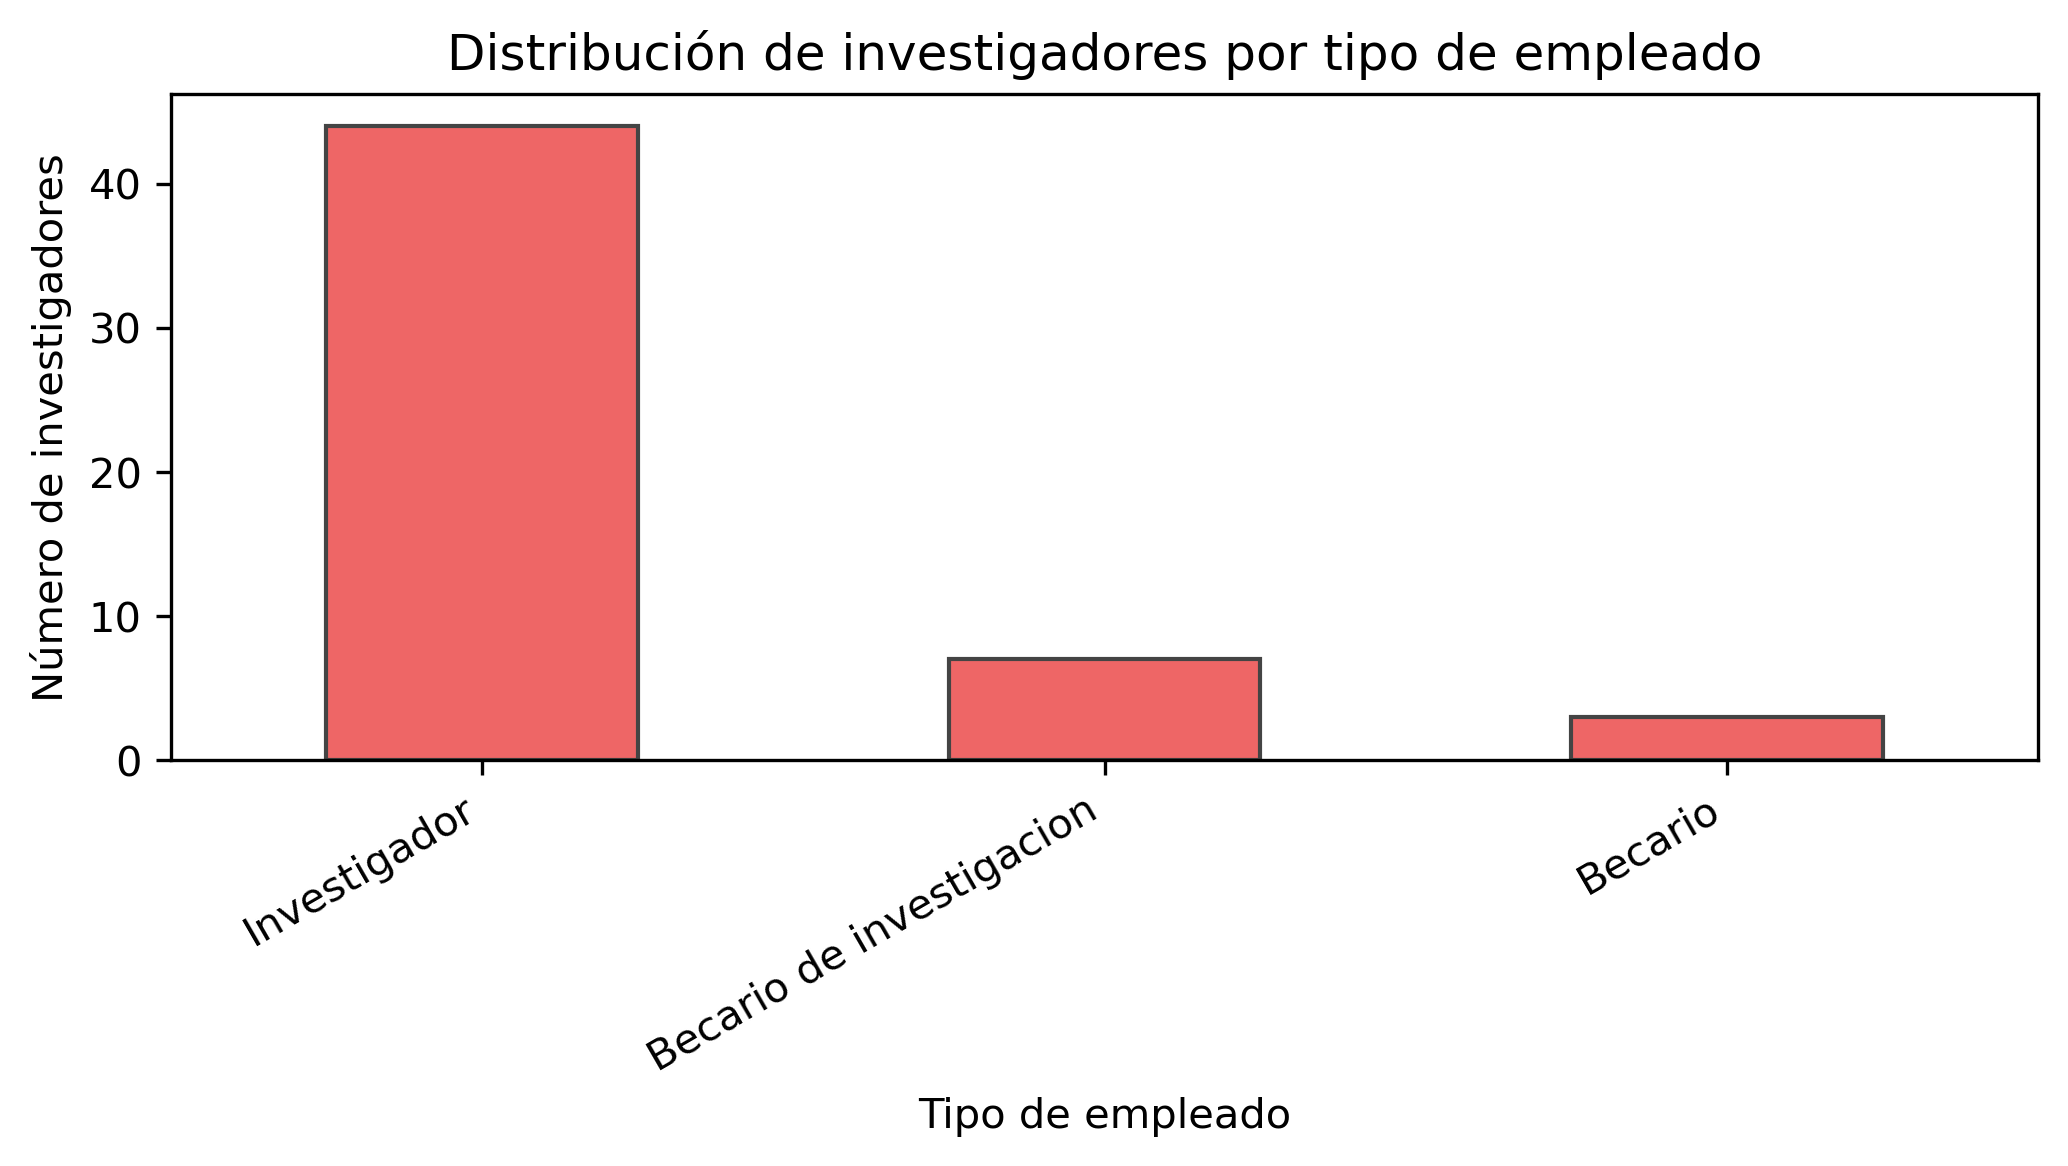
\includegraphics[width=0.7\textwidth]{imgs/eda_tipo_empleado.png}
\caption{Distribución de investigadores por tipo de empleado.}
\label{fig:eda_tipo_empleado}
\end{figure}

La distribución por áreas de trabajo se presenta en la Figura~\ref{fig:eda_areas_trabajo}. En este caso, el gráfico representa asociaciones investigador-área, no una partición estricta de los investigadores, ya que una misma persona puede aparecer vinculada a más de un área. Las áreas con mayor número de asociaciones son Matemática aplicada y Análisis, seguidas por Ciencia de Datos y Becarios.

\begin{figure}[H]
\centering

\includegraphics[width=0.6\textwidth]{imgs/eda_areas_trabajo.png}
\caption{Distribución de asociaciones investigador-área por área de trabajo.}
\label{fig:eda_areas_trabajo}
\end{figure}

\subsection{Artículos y revistas}

En relación con la producción académica recopilada, la Figura~\ref{fig:eda_articulos_revistas} muestra la relación entre el número de artículos asociados a cada investigador y el número de revistas distintas en las que aparecen dichos artículos. En términos generales, se observa una relación creciente entre ambas variables: los investigadores con mayor número de artículos tienden también a estar asociados a un mayor número de revistas. No obstante, la dispersión de los puntos muestra que esta relación no es completamente uniforme, ya que existen diferencias en la concentración de revistas asociadas a cada investigador.

\begin{figure}[H]
\centering
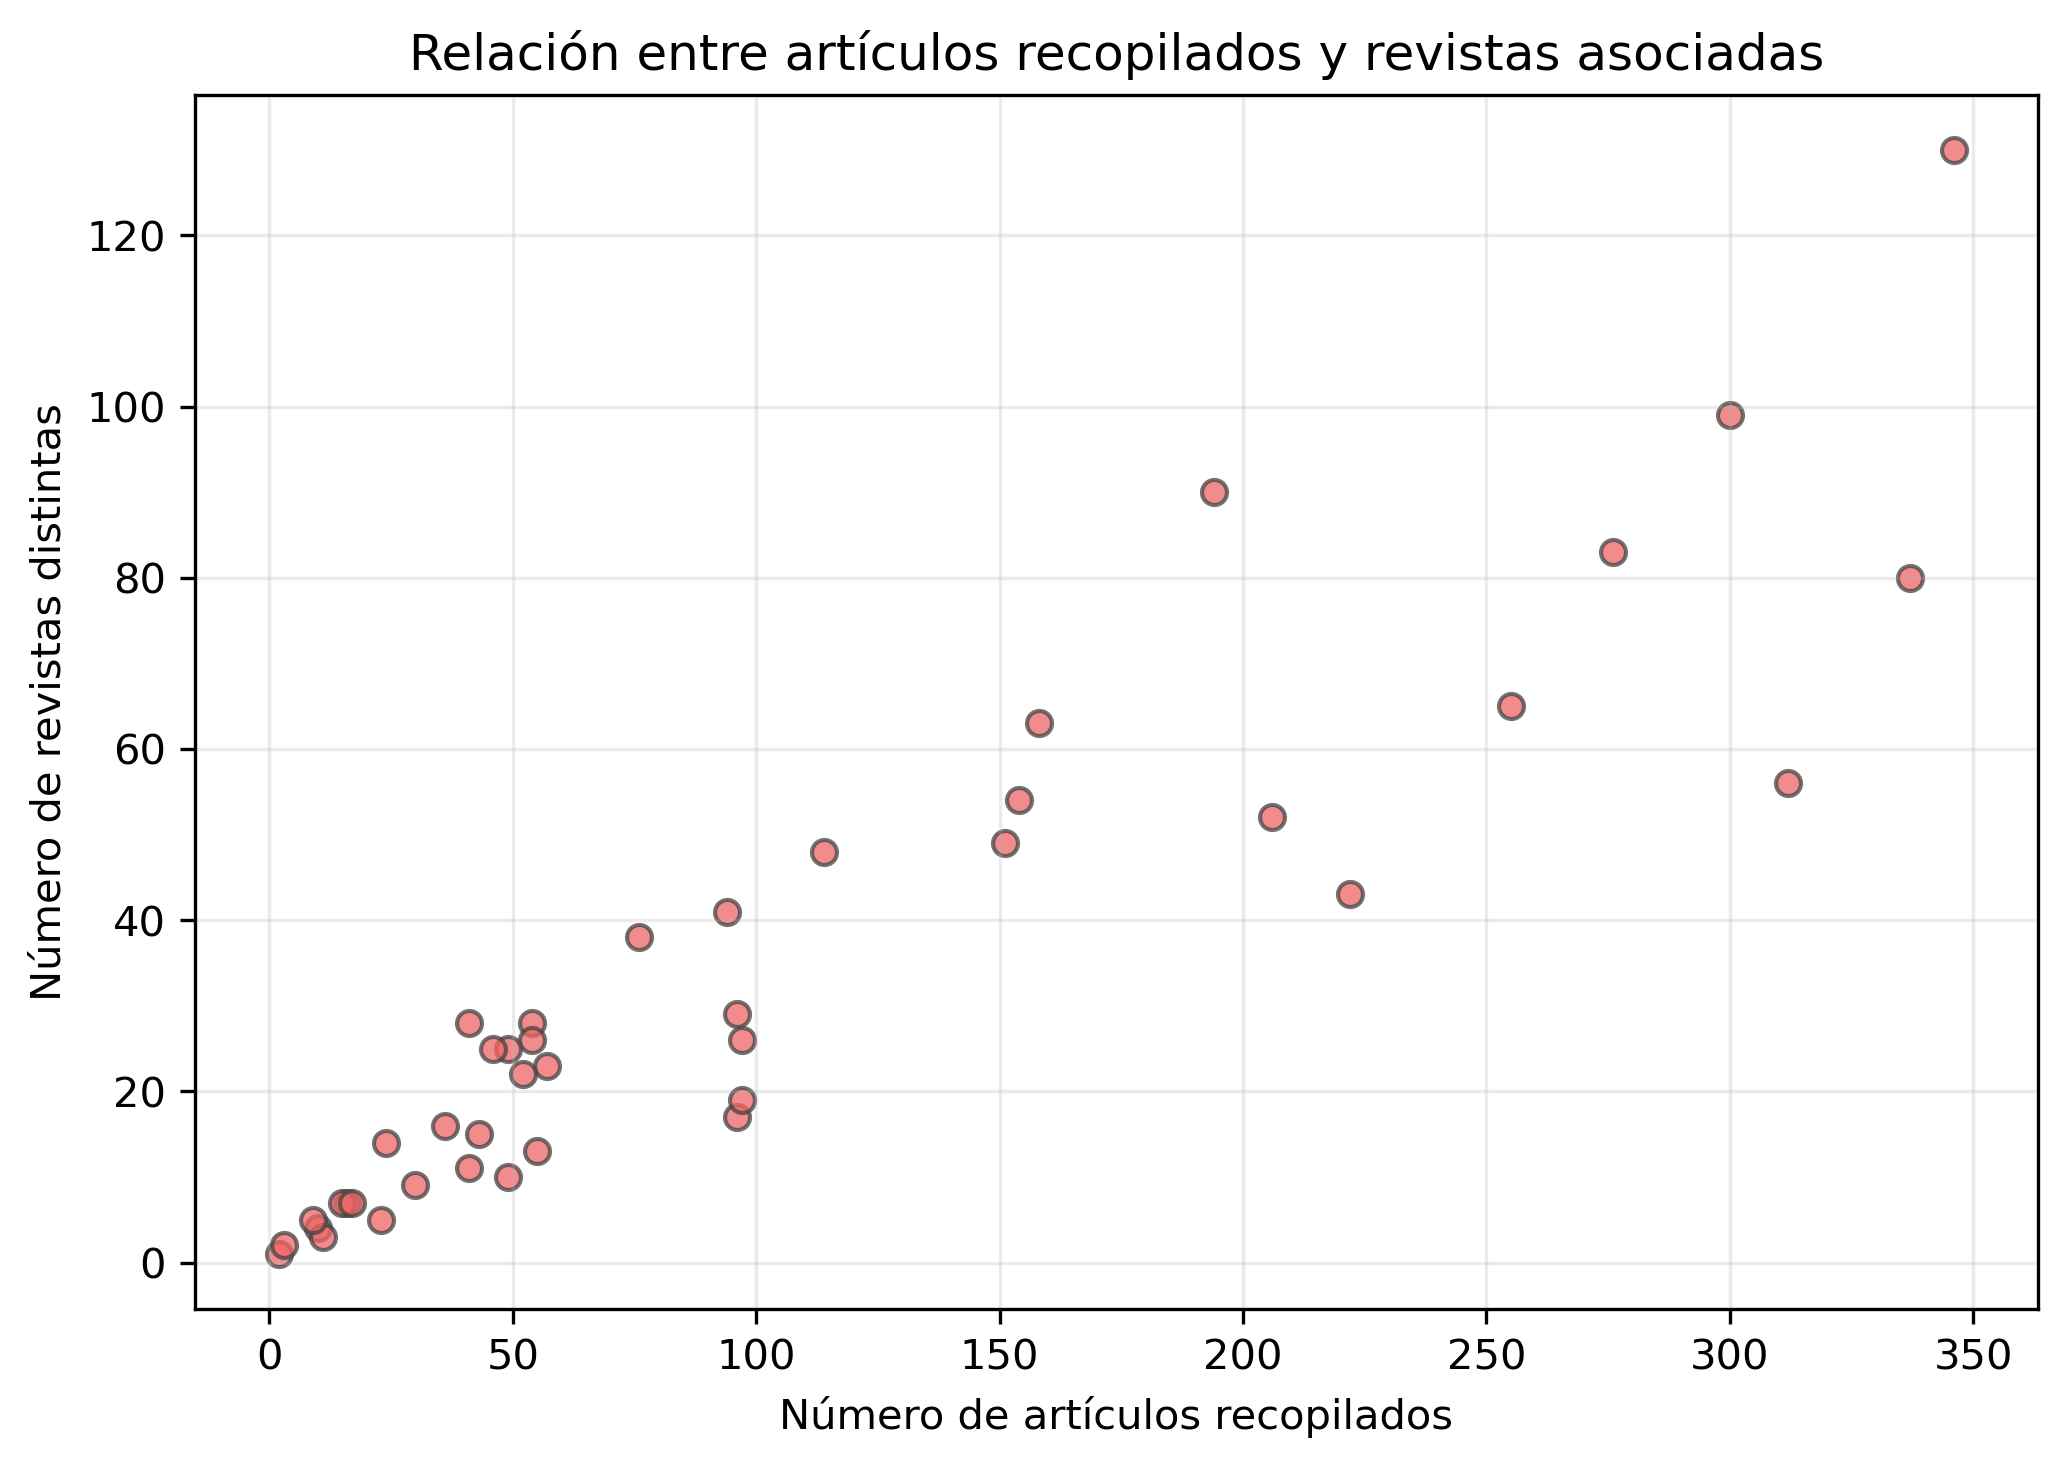
\includegraphics[width=0.6\textwidth]{imgs/eda_articulos_vs_revistas.png}
\caption{Relación entre artículos recopilados y revistas distintas asociadas por investigador.}
\label{fig:eda_articulos_revistas}
\end{figure}

Además de analizar la relación entre artículos y revistas, se revisó la distribución de las revistas según su editorial. La Figura~\ref{fig:eda_top_editoriales} muestra las quince editoriales con mayor número de revistas dentro de la base de datos. Se observa que Elsevier y Springer concentran una parte destacada de las revistas recopiladas, seguidas a mayor distancia por editoriales como MDPI y Taylor \& Francis.

\begin{figure}[H]
\centering
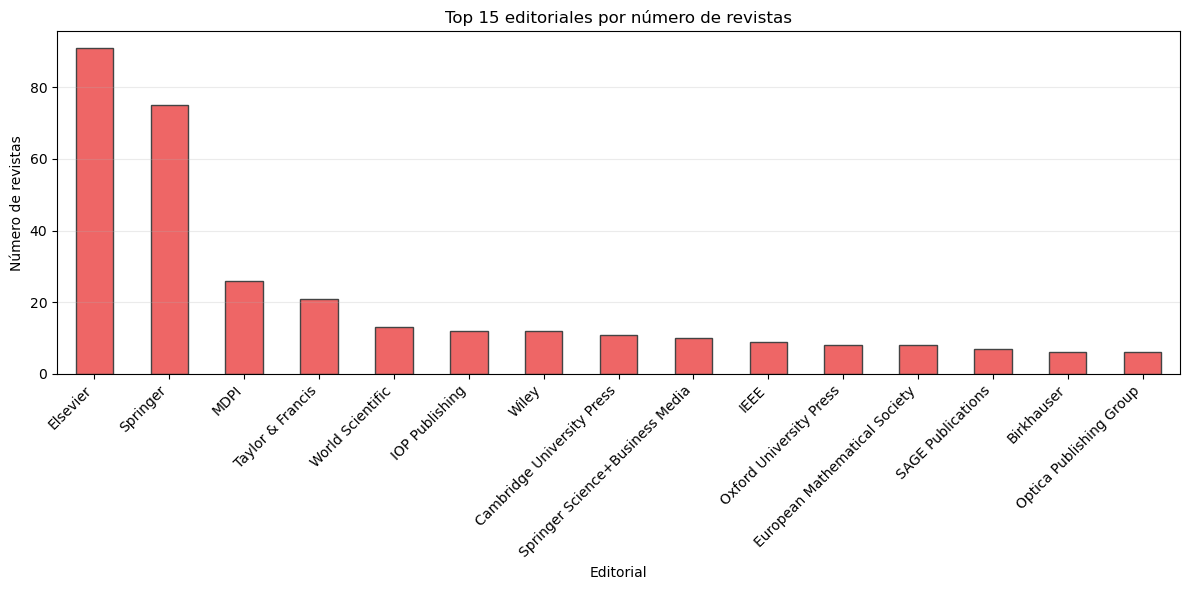
\includegraphics[width=0.9\textwidth]{imgs/eda_top_editoriales.png}
\caption{Principales editoriales asociadas a las revistas recopiladas.}
\label{fig:eda_top_editoriales}
\end{figure}

Esta distribución permite describir la composición de la entidad revista y comprobar que la base recoge publicaciones procedentes de editoriales científicas diversas. No obstante, el gráfico debe interpretarse únicamente como una descripción agregada de la base de datos, no como una valoración de la calidad de las revistas ni de la producción de los investigadores.

\subsection{Actividad en proyectos de investigación}

Para comparar las principales dimensiones de información asociadas a cada investigador, la Figura~\ref{fig:eda_distribuciones_investigador} resume la variabilidad de la información asociada a cada investigador. Los diagramas de caja muestran que el número de artículos y revistas recopilados presenta una dispersión elevada: la mayoría de investigadores se concentra en valores moderados, mientras que algunos casos alcanzan valores considerablemente superiores. En cambio, los proyectos asociados presentan una distribución más compacta. Esta diferencia refleja que la cobertura de publicaciones y revistas es más variable entre investigadores que la información relativa a proyectos, por lo que los resultados derivados de la base deben interpretarse teniendo en cuenta esta heterogeneidad.

\begin{figure}[H]
\centering
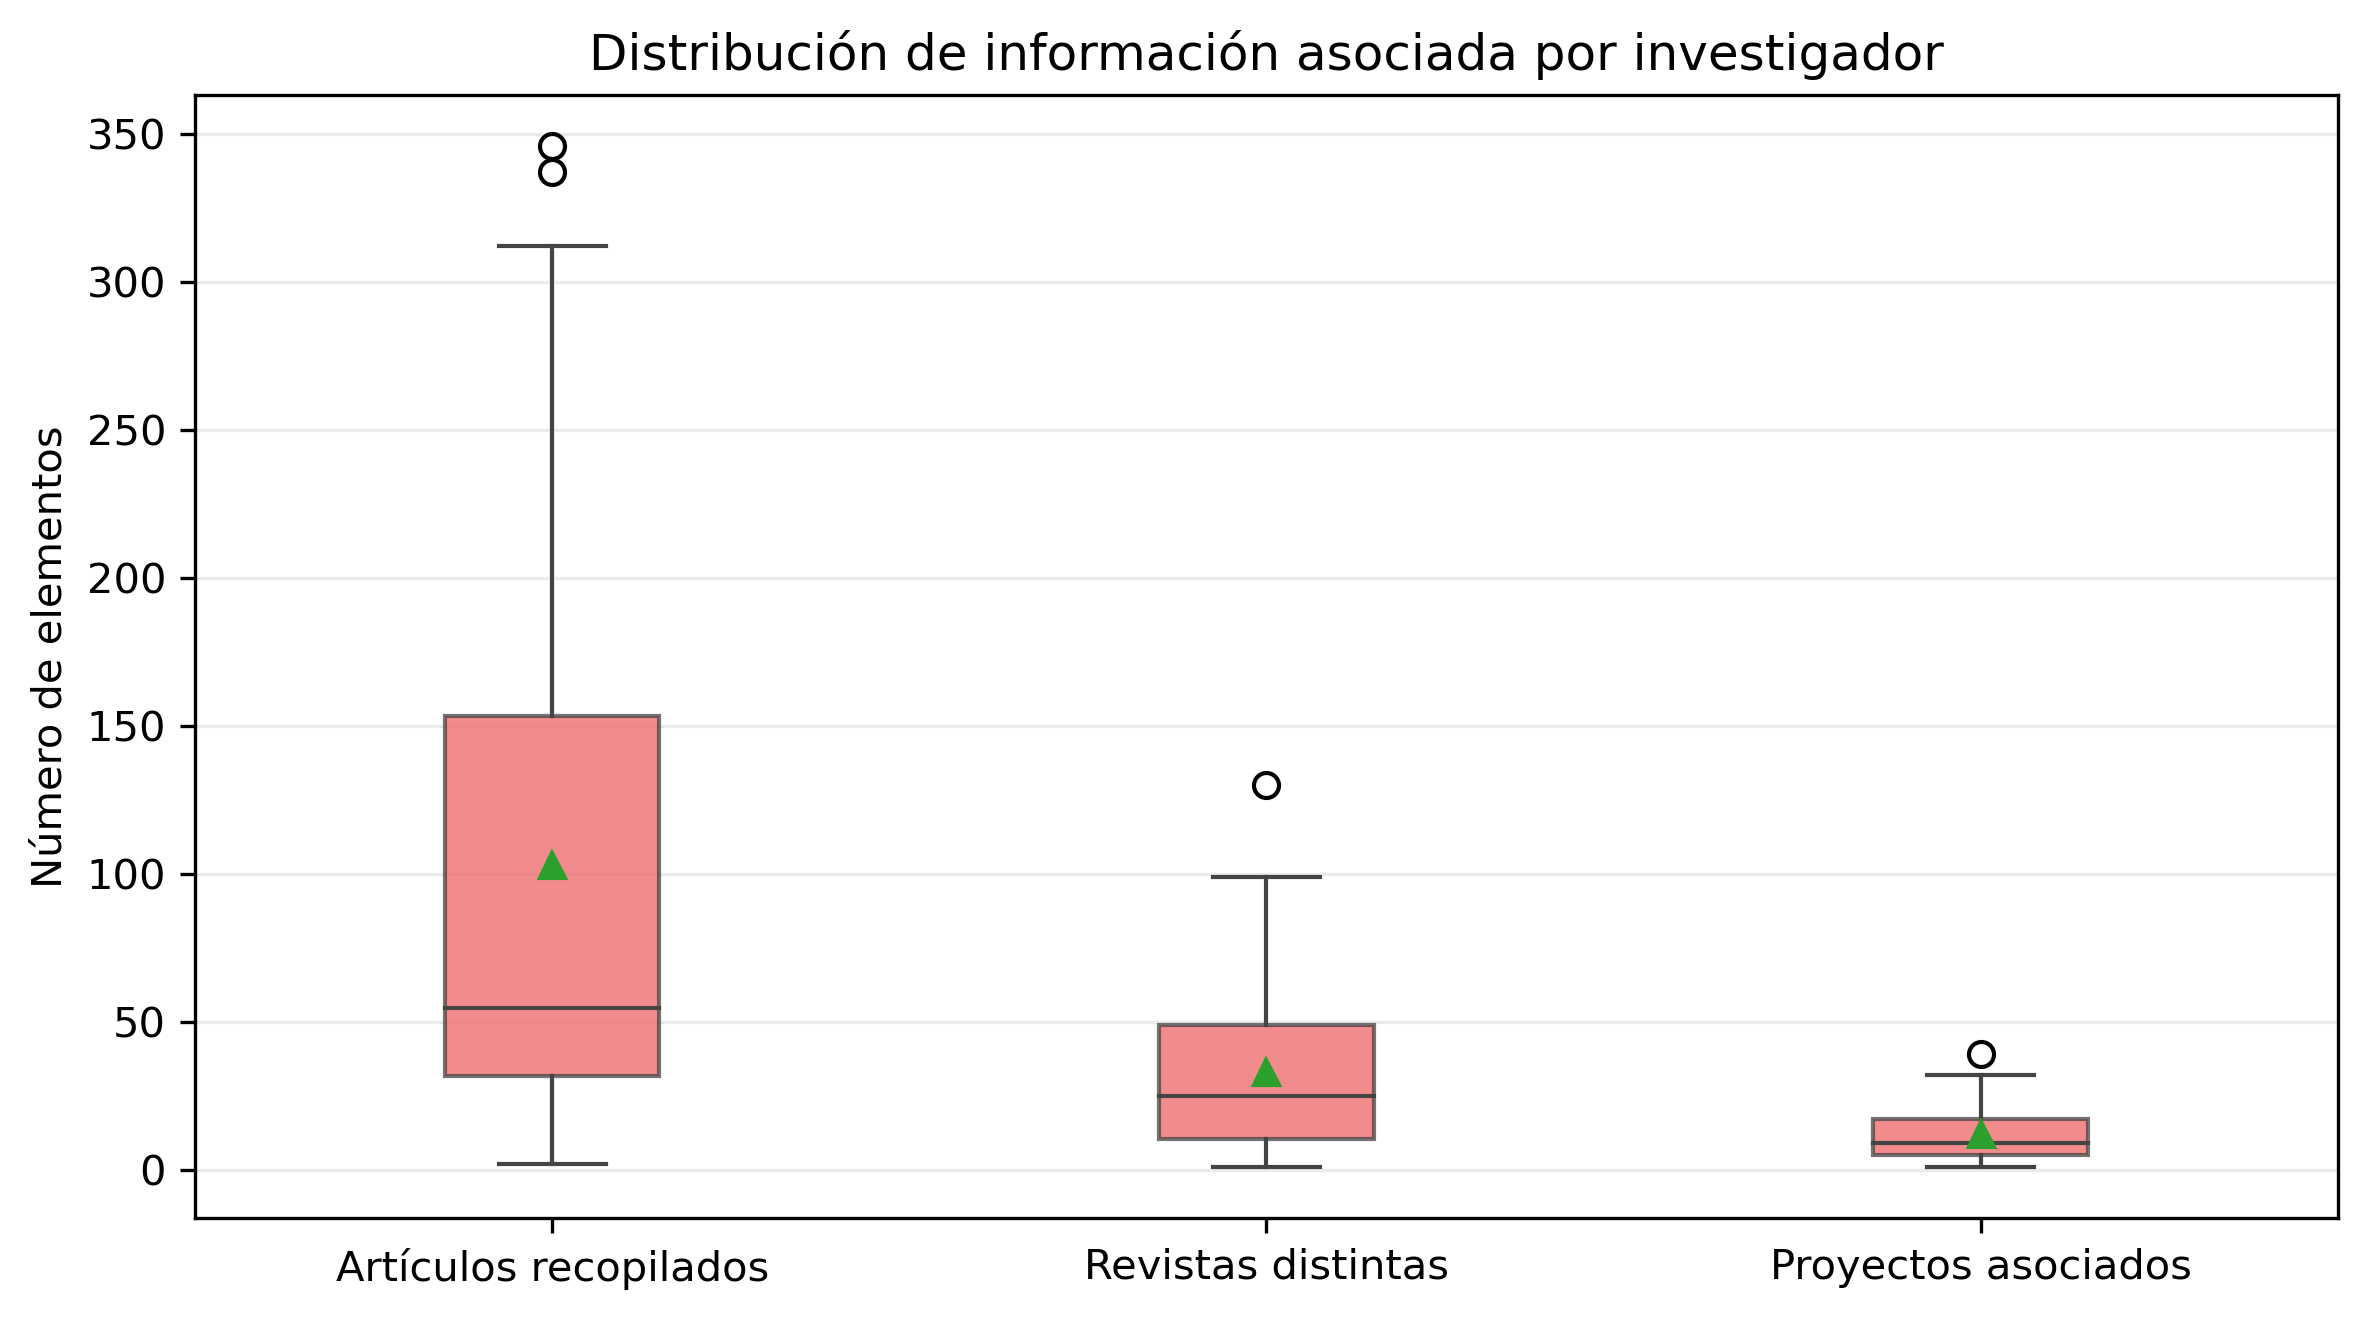
\includegraphics[width=0.7\textwidth]{imgs/eda_distribuciones_por_investigador.png}
\caption{Distribución de artículos, revistas distintas y proyectos asociados por investigador.}
\label{fig:eda_distribuciones_investigador}
\end{figure}

En los proyectos, se analizó cuántos investigadores internos del IUMPA estaban asociados a cada proyecto registrado. La Figura~\ref{fig:eda_investigadores_proyecto} muestra que la mayoría aparecen vinculados a un único investigador interno, aunque esto no implica que sean proyectos individuales, ya que el conteo no incluye participantes externos ni investigadores fuera del alcance del modelo. En concreto, 163 proyectos están asociados a un solo investigador interno del IUMPA, 54 a dos, 31 a tres, 26 a entre cuatro y cinco, 6 a entre seis y diez, y solo uno a más de diez. Esta distribución permite observar la presencia interna del IUMPA en los proyectos recopilados y detectar aquellos casos en los que varios miembros del instituto coinciden en un mismo trabajo.

\begin{figure}[H]
\centering
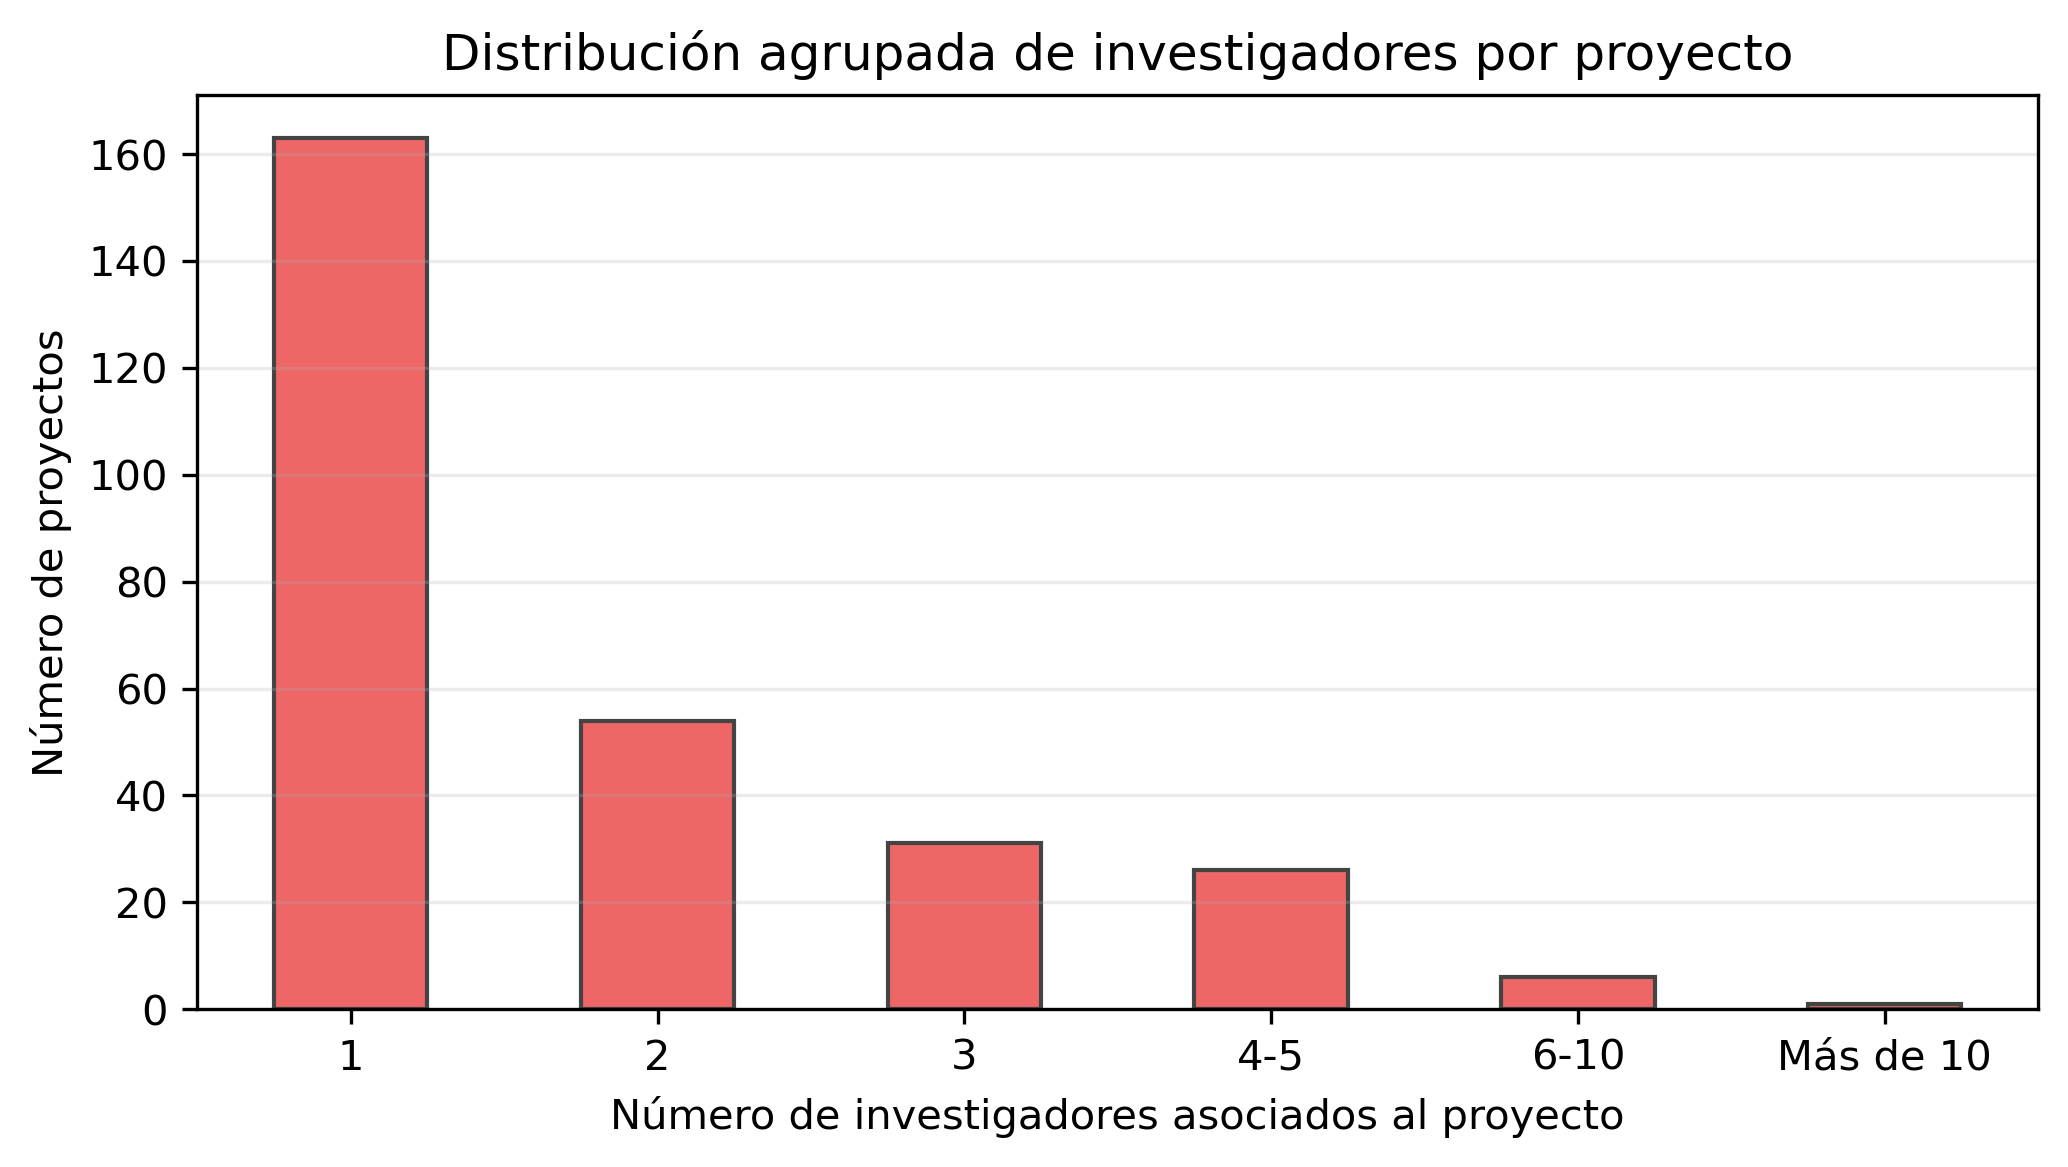
\includegraphics[width=0.6\textwidth]{imgs/eda_investigadores_por_proyecto_agrupado.png}
\caption{Distribución agrupada del número de investigadores internos del IUMPA asociados a cada proyecto.}
\label{fig:eda_investigadores_proyecto}
\end{figure}

Además de analizar cuántos investigadores internos aparecen asociados a cada proyecto, se revisó la distribución temporal de los proyectos recopilados. La Figura~\ref{fig:eda_proyectos_anio} muestra el número de proyectos únicos registrados por año, lo que permite observar cómo se distribuye esta información a lo largo del periodo cubierto por la base de datos.

\begin{figure}[H]
\centering
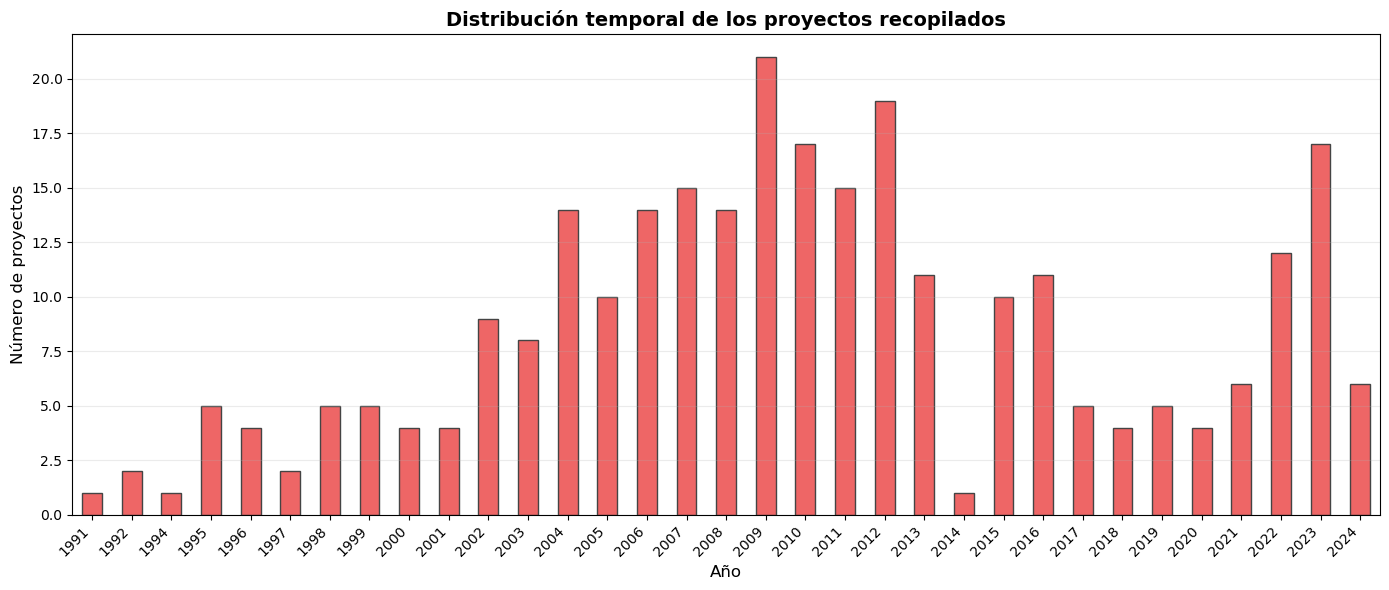
\includegraphics[width=\textwidth]{imgs/distr_temporal_proyectos.png}
\caption{Distribución temporal de los proyectos asociados a investigadores del IUMPA.}
\label{fig:eda_proyectos_anio}
\end{figure}

La distribución muestra una mayor concentración de proyectos en determinados periodos, especialmente alrededor de los años 2009, 2010 y 2012, así como un nuevo incremento en los años más recientes. Esta visualización complementa el análisis anterior, ya que permite describir no solo cuántos proyectos se han recopilado y cuántos investigadores internos aparecen vinculados a ellos, sino también cómo se reparte temporalmente la información disponible.

\subsection{Cobertura de la información temática}

Finalmente, la parte semántica de la base de datos también presenta una cobertura suficiente para servir como punto de partida al análisis posterior. A partir de las revistas recopiladas se construyeron estructuras auxiliares basadas en palabras clave, cuyos principales valores se resumen en la Tabla~\ref{tab:cobertura_semantica}.

\begin{table}[H]
\centering
\small
\begin{tabular}{lr}
\toprule
\textbf{Elemento} & \textbf{Valor} \\
\midrule
Palabras clave únicas & 103 \\
Revistas con representación temática & 643 \\
Investigadores con representación temática & 42 \\
Relaciones investigador-palabra clave activas & 1916 \\
Relaciones revista-palabra clave activas & 4410 \\
\bottomrule
\end{tabular}
\caption{Cobertura de las estructuras semánticas generadas.}
\label{tab:cobertura_semantica}
\end{table}

Estos valores indican que las estructuras semánticas generadas ofrecen cobertura suficiente para construir las representaciones temáticas utilizadas en el análisis posterior.

\section{Valoración de la base de datos construida}

La valoración de la base de datos construida debe hacerse desde su función dentro del proyecto y desde su utilidad como recurso reutilizable. Su principal aportación no reside únicamente en reunir información procedente de distintas fuentes, sino en haberla organizado de forma que pudiera ser utilizada posteriormente para la visualización interactiva, para el análisis semántico y para posibles consultas, actualizaciones o ampliaciones futuras por parte del IUMPA.

Desde el punto de vista del modelo, la estructura final resultó adecuada para los objetivos planteados, ya que permitió representar entidades como investigadores, revistas, áreas y proyectos, así como relaciones derivadas de publicaciones, participación en proyectos y colaboraciones. De este modo, la base de datos se consolidó como una estructura preparada para generar los grafos interactivos y para consultar la actividad investigadora del IUMPA desde una perspectiva relacional.

Además, la información de revistas permitió construir estructuras auxiliares basadas en palabras clave, orientadas a representar temáticamente a los investigadores. Por tanto, esta base de datos también ofrecía un punto de partida adecuado para abordar el análisis semántico desarrollado en la segunda parte del trabajo.

No obstante, su interpretación debe realizarse teniendo en cuenta las limitaciones propias del proceso de recopilación. La información procedía de fuentes públicas con distintos formatos, niveles de detalle y grados de completitud, por lo que la ausencia de un registro no debe interpretarse necesariamente como ausencia de actividad investigadora. En este sentido, la base construida debe entenderse como una estructura útil y ampliable, pero condicionada por la información disponible y por las decisiones de depuración adoptadas durante el proyecto.

Finalmente, dado que la base de datos puede servir como punto de partida para futuras consultas, actualizaciones o ampliaciones, resulta necesario documentar su estructura de forma clara. Por ello, el Apéndice~\ref{ap:diccionario_datos} recoge una descripción de los principales ficheros generados, sus atributos más relevantes y algunos ejemplos visuales de su organización.

%%%%%%%%%%%%%%%%%%%%%%%%%%%%%%%%%%%%%%%%%%%%%%%%%%%%%%%%%%%%%%%%%%%%%%%%%%%%%%%

%%%%%%%%%%%
%Capítulo 5
%%%%%%%%%%%

\chapter{Desarrollo de la aplicación interactiva}

La base de datos construida proporcionaba una estructura organizada de la información, pero su consulta mediante ficheros tabulares no permitía aprovechar la dimensión relacional del proyecto. Para interpretar de forma más intuitiva las relaciones entre investigadores, revistas y proyectos, así como las colaboraciones recogidas en la base de datos, era conveniente trasladar esa información a un entorno visual e interactivo.

Por este motivo, se desarrolló una aplicación interactiva en R mediante Shiny \cite{shiny}. La herramienta permitió convertir las entidades y relaciones definidas previamente en grafos explorables, de forma que el usuario pudiera consultar visualmente la estructura de la información sin necesidad de acceder directamente a los ficheros de datos.

La aplicación se organizó en torno a distintos grafos interactivos, cada uno orientado a representar una parte concreta de la información recopilada. Su desarrollo implicó definir la estructura general de la herramienta, transformar los datos tabulares en nodos y relaciones visuales, e incorporar elementos de interacción que facilitaran la exploración de la información.

\section{Diseño general de la herramienta}

La aplicación se estructuró como una herramienta desarrollada en R mediante Shiny, organizada a partir de la separación entre la lectura de datos, el procesamiento de la información y la generación de componentes visuales. Esta organización permitió mantener una correspondencia clara entre los ficheros de la base de datos y los grafos mostrados al usuario.

De esta forma, la herramienta puede entenderse a partir de tres fases principales:

\begin{itemize}
    \item \textbf{Fase de lectura de los ficheros}: en la que se cargaban las entidades y relaciones necesarias para construir las visualizaciones.

    \item \textbf{Lógica de procesamiento}: encargada de adaptar esos datos al formato requerido por los grafos, diferenciando los elementos que debían representarse como nodos y las conexiones que debían representarse como enlaces.

    \item \textbf{Interfaz visual}: destinada a consultar los grafos resultantes y acceder a la información asociada a los elementos representados.
\end{itemize}

Los ficheros construidos previamente actuaban como entrada del sistema, mientras que la aplicación se encargaba de interpretarlos y convertirlos en representaciones visuales interactivas. De este modo, los cambios en los datos podían incorporarse con mayor facilidad, siempre que se mantuviera la estructura esperada por la herramienta.

El diseño de la aplicación estuvo condicionado por el objetivo exploratorio del proyecto. No se buscaba construir una plataforma cerrada de consulta estadística, sino una herramienta que permitiera navegar por la información recopilada y observar las relaciones existentes entre investigadores, revistas y proyectos, así como las colaboraciones derivadas de publicaciones y proyectos compartidos. Además, se incorporó la posibilidad de filtrar las visualizaciones por áreas de trabajo, utilizando la relación previamente definida entre investigadores y áreas. Por ello, la organización general de la herramienta se orientó a facilitar una exploración visual progresiva, desde una visión global de las relaciones hasta la consulta de información concreta asociada a cada elemento.

Desde el punto de vista de implementación, la aplicación siguió la estructura habitual de Shiny, separando la definición de la interfaz de usuario de la lógica encargada de procesar los datos y generar las visualizaciones. Esta separación facilitó mantener diferenciadas la parte visual de la aplicación y la lógica encargada de preparar los datos para su representación gráfica.

\section{Construcción de los grafos interactivos}

La construcción de los grafos interactivos consistió en transformar las entidades y relaciones de la base de datos en estructuras visuales formadas por nodos y enlaces. Los nodos representaban los elementos del sistema que se querían visualizar, mientras que los enlaces indicaban las relaciones existentes entre ellos. De esta forma se transformaron los ficheros tabulares descritos anteriormente en visualizaciones orientadas a explorar la actividad investigadora del IUMPA.

El proceso seguido para construir cada grafo mantuvo una lógica común. En primer lugar, se seleccionaban los ficheros necesarios para cada visualización. A partir de ellos se identificaban los elementos que debían representarse como nodos y las conexiones que debían convertirse en enlaces. Posteriormente, los datos se adaptaban al formato requerido por la librería de visualización utilizada en la aplicación, Apache ECharts \cite{echarts}, incorporando la información necesaria para mostrar etiquetas, categorías y atributos asociados a cada elemento.

En el caso de los investigadores, también se conservó su asociación con las áreas de trabajo, no como nodos independientes del grafo, sino como atributo utilizado posteriormente para filtrar las visualizaciones.

Uno de los grafos principales de la aplicación permitió representar la relación entre investigadores y revistas a partir de los artículos recopilados. Esta visualización se construyó a partir de la relación \textit{ha\_publicado\_en}, utilizando como nodos los investigadores y las revistas, y como enlaces las relaciones que conectaban a cada investigador con los medios en los que aparecían sus artículos. En este caso, el grafo permitía observar la distribución de la producción académica recopilada y explorar qué revistas aparecían asociadas a cada investigador.

\begin{figure}[H]
\centering
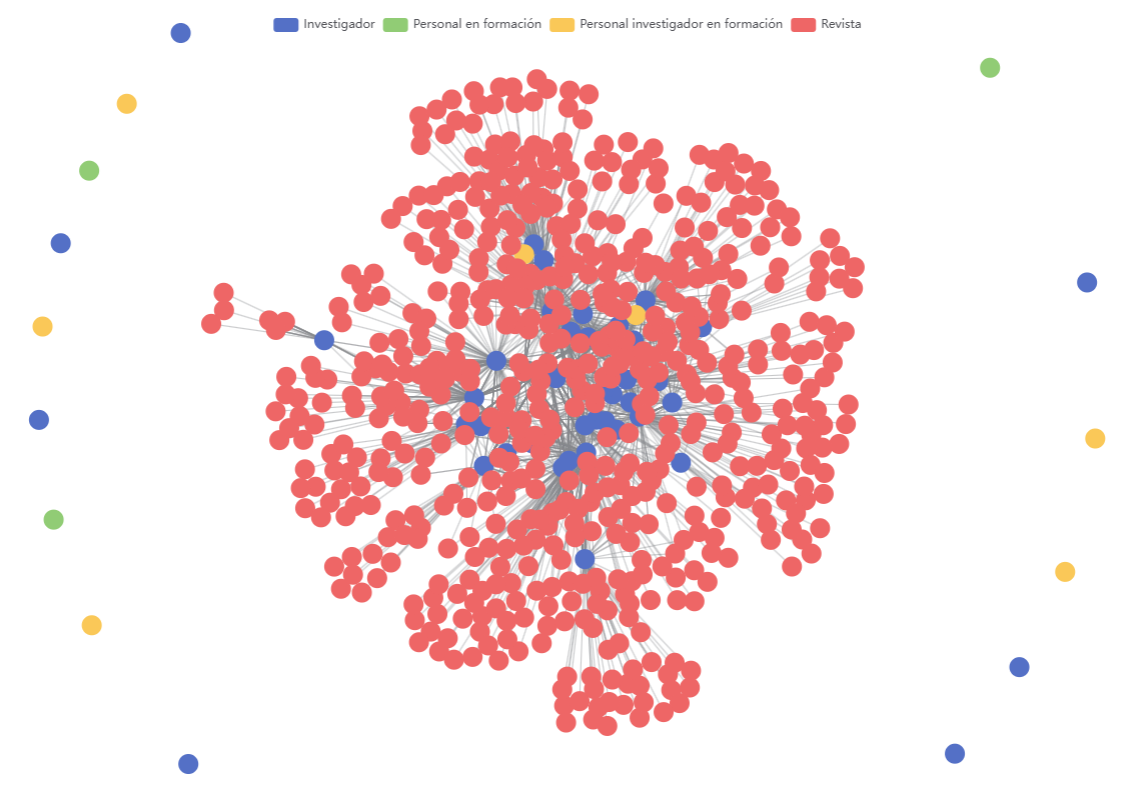
\includegraphics[width=0.8\textwidth]{imgs/inv_vs_revistas.png}
\caption{Grafo de relación entre investigadores y revistas.}
\label{fig:grafo_investigadores_revistas}
\end{figure}

La información relativa a proyectos se representó mediante un grafo específico basado en la relación \textit{ha\_participado\_en}. Esta visualización utilizaba como nodos los investigadores y los proyectos, y como enlaces la participación de cada investigador en los proyectos registrados. Este grafo permitía explorar una dimensión de la actividad investigadora distinta a la derivada de los artículos, identificando qué investigadores aparecían vinculados a proyectos concretos. Para simplificar la visualización, los proyectos se mostraron a partir de su título, de forma que registros con el mismo nombre quedaban consolidados en un único nodo visual.
 
\begin{figure}[H]
\centering
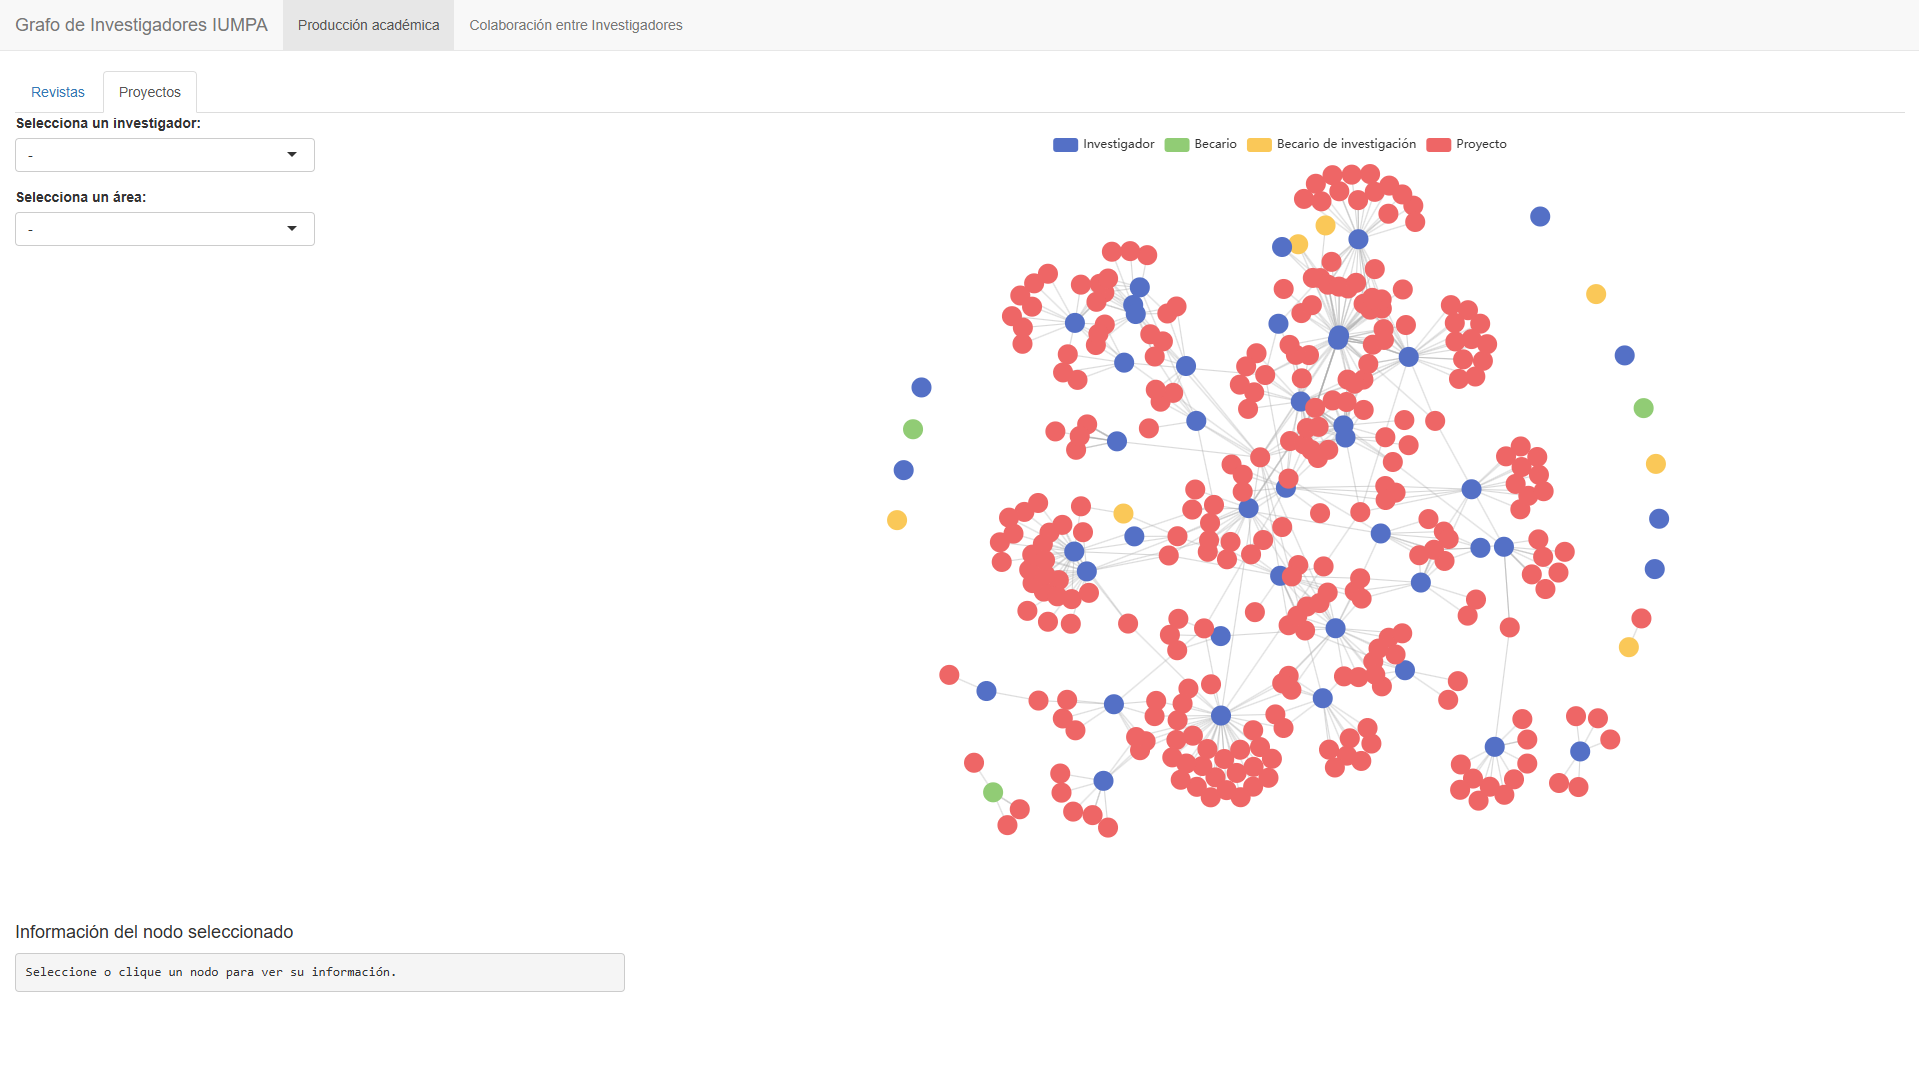
\includegraphics[width=0.8\textwidth]{imgs/inv_vs_proyectos.png}
\caption{Grafo de relación entre investigadores y proyectos de investigación.}
\label{fig:grafo_investigadores_proyectos}
\end{figure}

Además de los grafos que relacionaban investigadores con otros tipos de entidades, la aplicación incorporó visualizaciones centradas en relaciones entre investigadores. A partir de la relación \textit{ha\_publicado\_con}, se construyó un grafo de colaboración basado en artículos compartidos. En este caso, los nodos representaban investigadores y los enlaces indicaban la existencia de publicaciones conjuntas entre ellos. Esta visualización permitía observar relaciones de coautoría y detectar conexiones derivadas de la producción académica recopilada.

\begin{figure}[H]
\centering
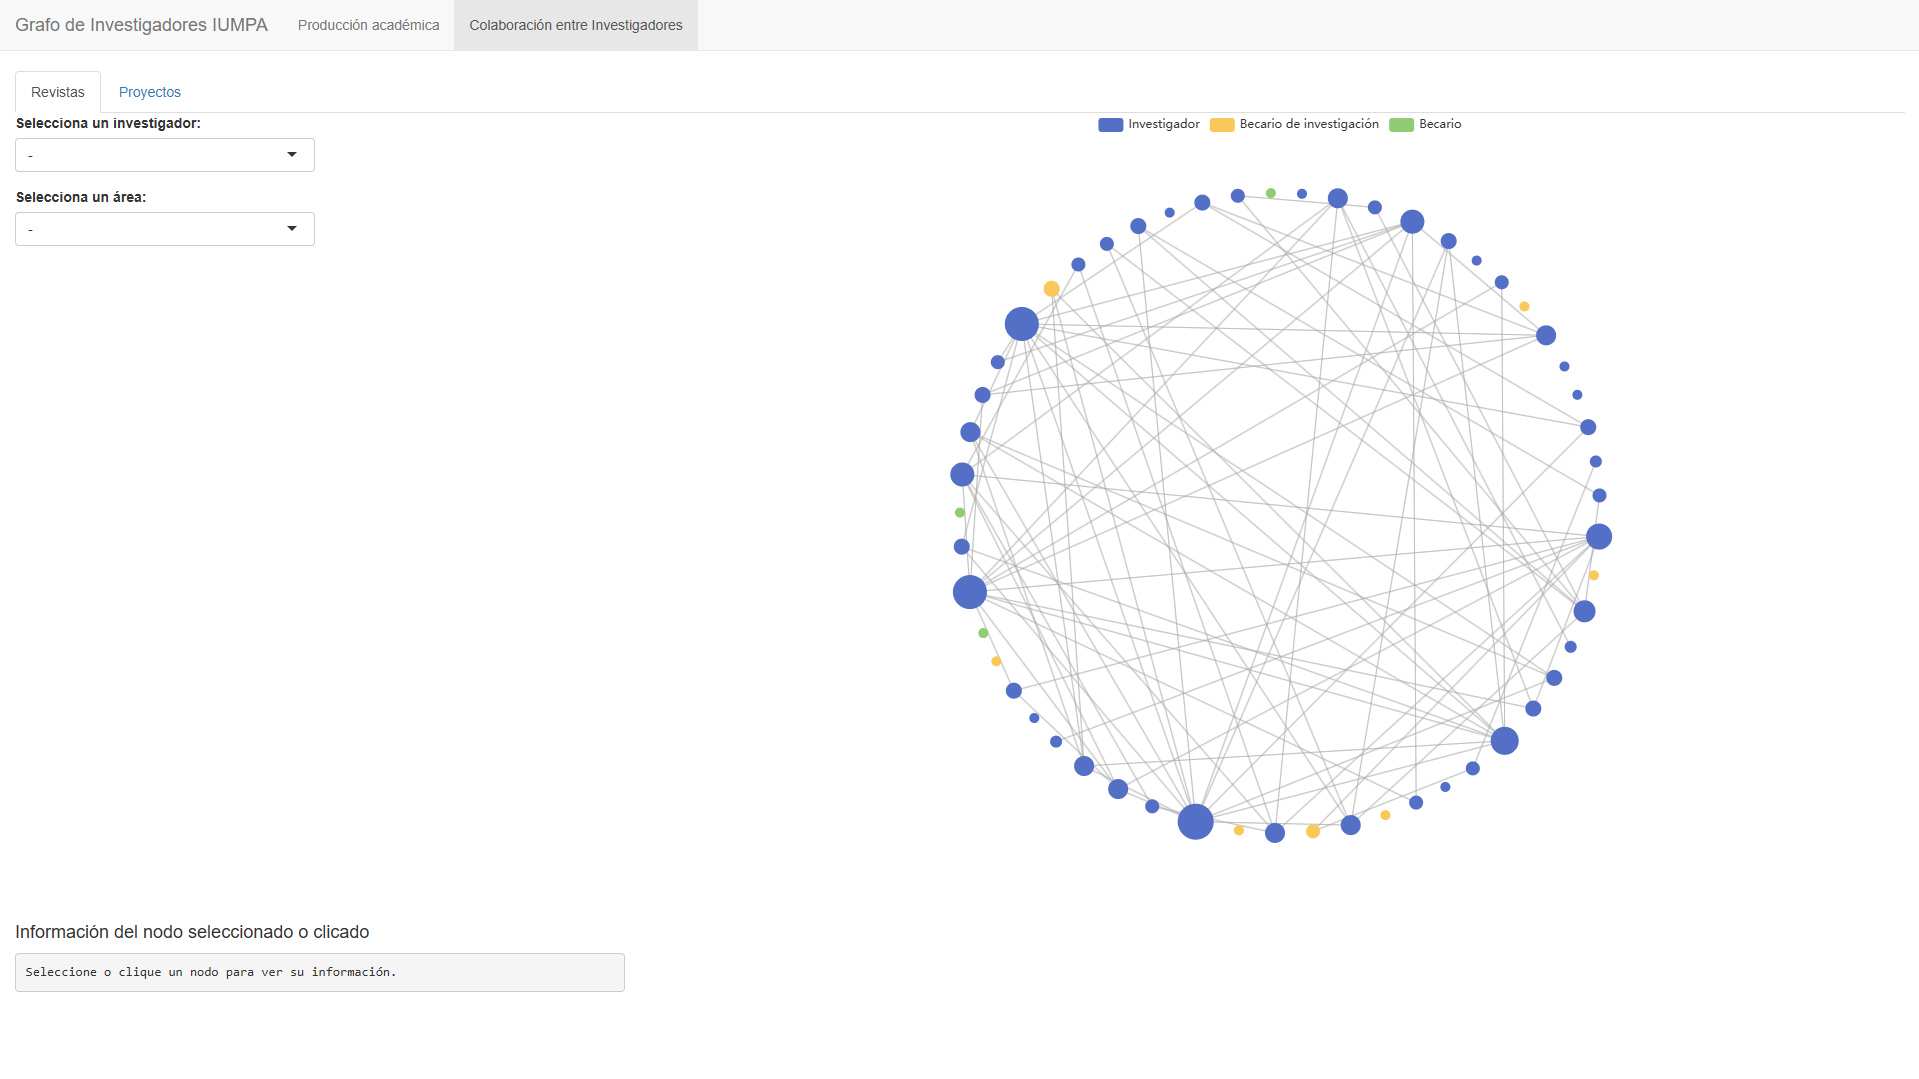
\includegraphics[width=0.8\textwidth]{imgs/inv_vs_inv_revistas.png}
\caption{Grafo de colaboración entre investigadores a partir de artículos compartidos.}
\label{fig:grafo_colaboracion_articulos}
\end{figure}

De forma análoga, la relación \textit{ha\_participado\_con} permitió representar colaboraciones derivadas de la participación conjunta en proyectos. En este grafo, los nodos representaban investigadores y los enlaces indicaban que dos investigadores aparecían asociados a un mismo proyecto. Esta visualización ofrecía una perspectiva complementaria a la colaboración basada en artículos y permitía diferenciar entre relaciones surgidas de la producción académica y relaciones derivadas de la participación común en proyectos de investigación.

\begin{figure}[H]
\centering
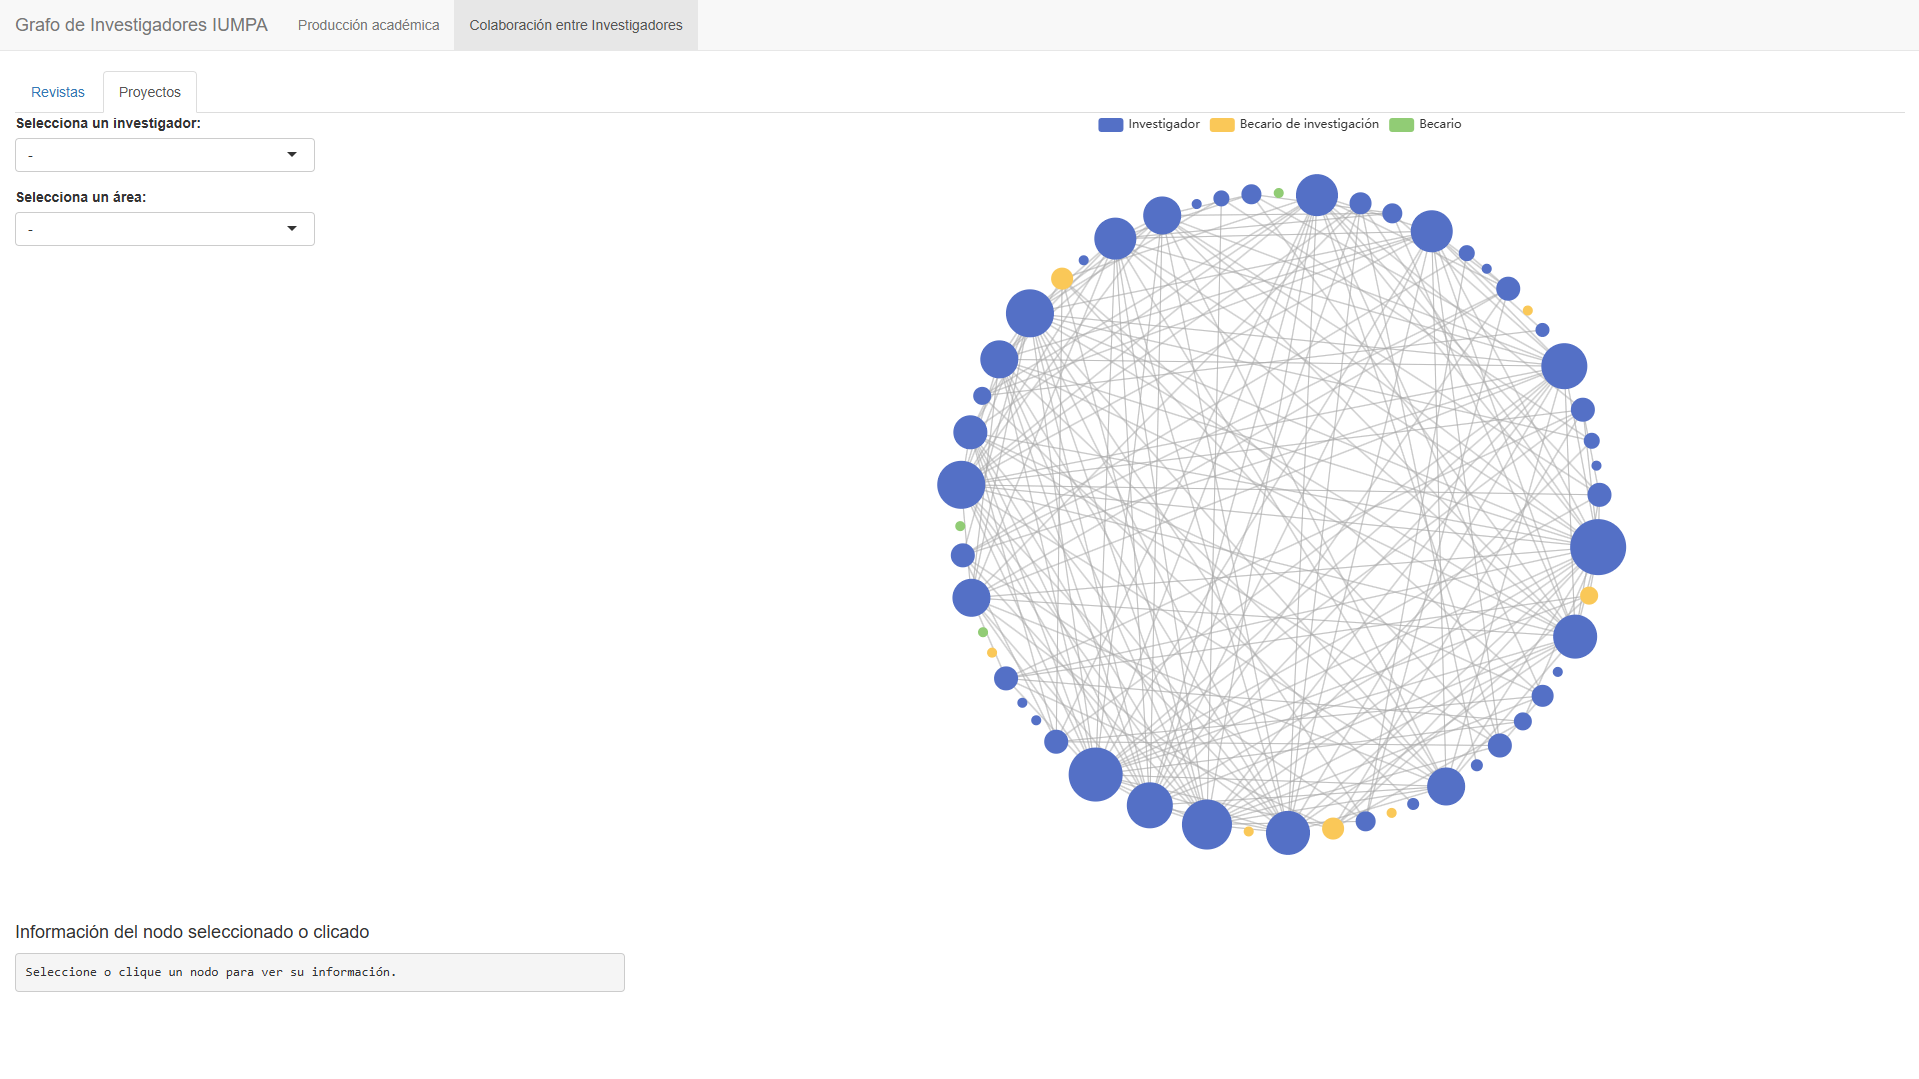
\includegraphics[width=0.8\textwidth]{imgs/inv_vs_inv_proyectos.png}
\caption{Grafo de colaboración entre investigadores a partir de la participación conjunta en proyectos.}
\label{fig:grafo_colaboracion_proyectos}
\end{figure}

La existencia de varios grafos permite evitar una única visualización excesivamente compleja. En lugar de representar todas las entidades y relaciones al mismo tiempo, la aplicación separa la información en vistas específicas: una centrada en la producción académica, otra en la participación en proyectos y otras dos en las relaciones de colaboración entre investigadores. Esta decisión facilita la interpretación de los resultados y permite que el usuario explore la información de forma progresiva.

\section{Elementos de interacción y visualización}

Además de construir los grafos interactivos, la aplicación incorporó distintos elementos de interacción y codificación visual para facilitar su exploración. El objetivo de estos elementos era permitir que el usuario pudiera pasar de una visión general de la red a consultas más concretas sobre los elementos representados, sin necesidad de consultar directamente los ficheros de datos.

Uno de los principales mecanismos de interacción fue el uso de selectores. En los cuatro grafos desarrollados se incorporaron controles que permitían filtrar la visualización por investigador y por área de trabajo, aunque su efecto dependía del tipo de grafo consultado:
\begin{itemize}
    \item \textbf{Producción académica}: el selector de investigador permitía mostrar únicamente las revistas o proyectos asociados a una persona concreta.

    \item \textbf{Colaboración entre investigadores}: permitía centrar la visualización en un investigador y en sus conexiones dentro de la red correspondiente.
\end{itemize}

Por su parte, el filtro por área permitía restringir la visualización a los investigadores asociados a una determinada línea de trabajo, junto con los elementos conectados a ellos cuando corresponda. De esta forma, el usuario podía reducir la complejidad de la red y analizar subconjuntos más manejables de la información.

\begin{figure}[H]
\centering
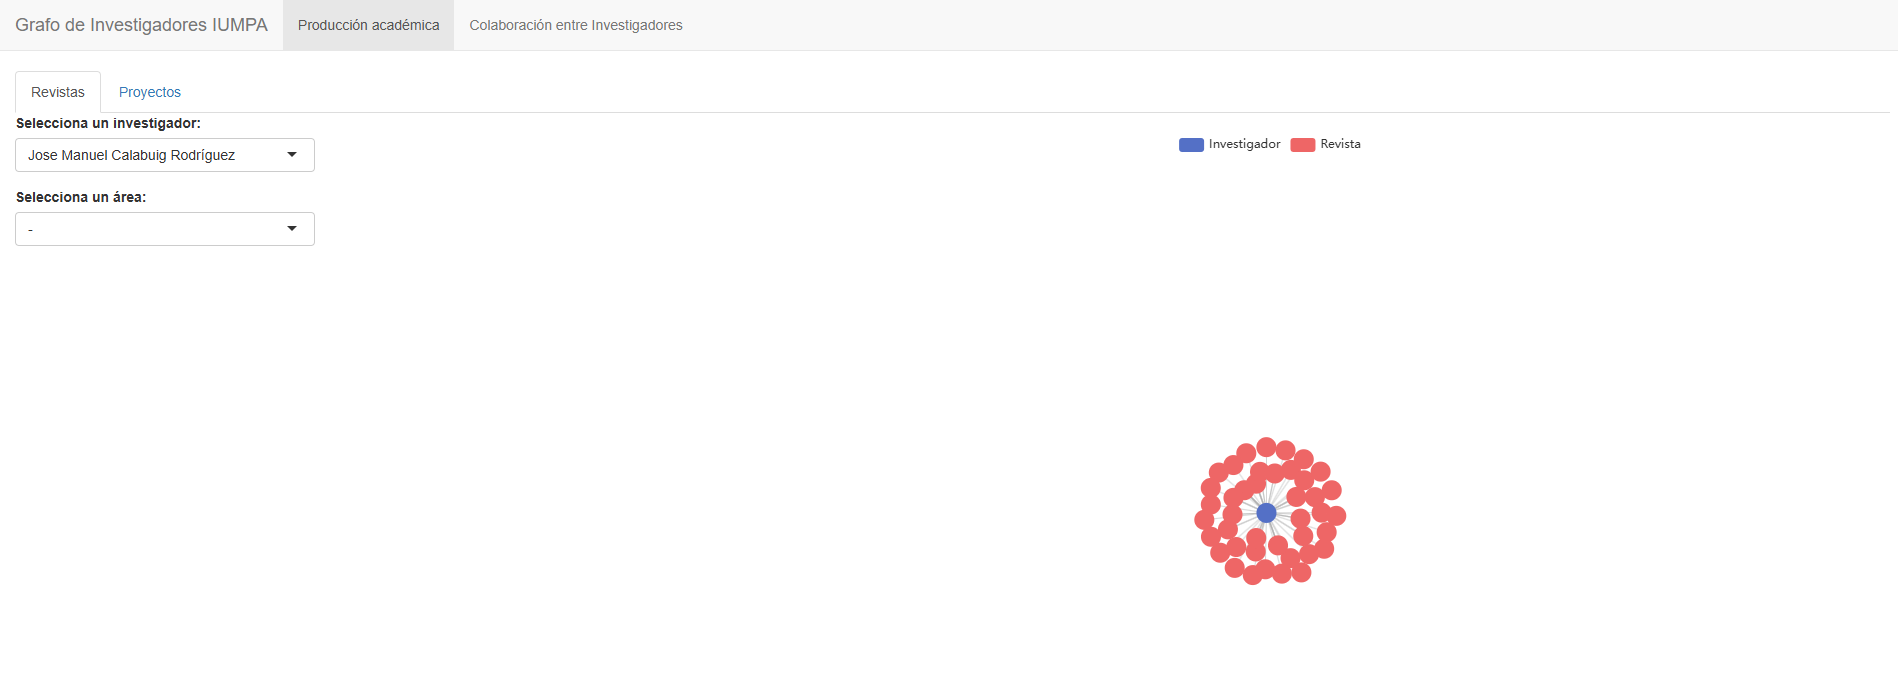
\includegraphics[width=0.48\textwidth]{imgs/filtrado_investigador.png}
\hfill
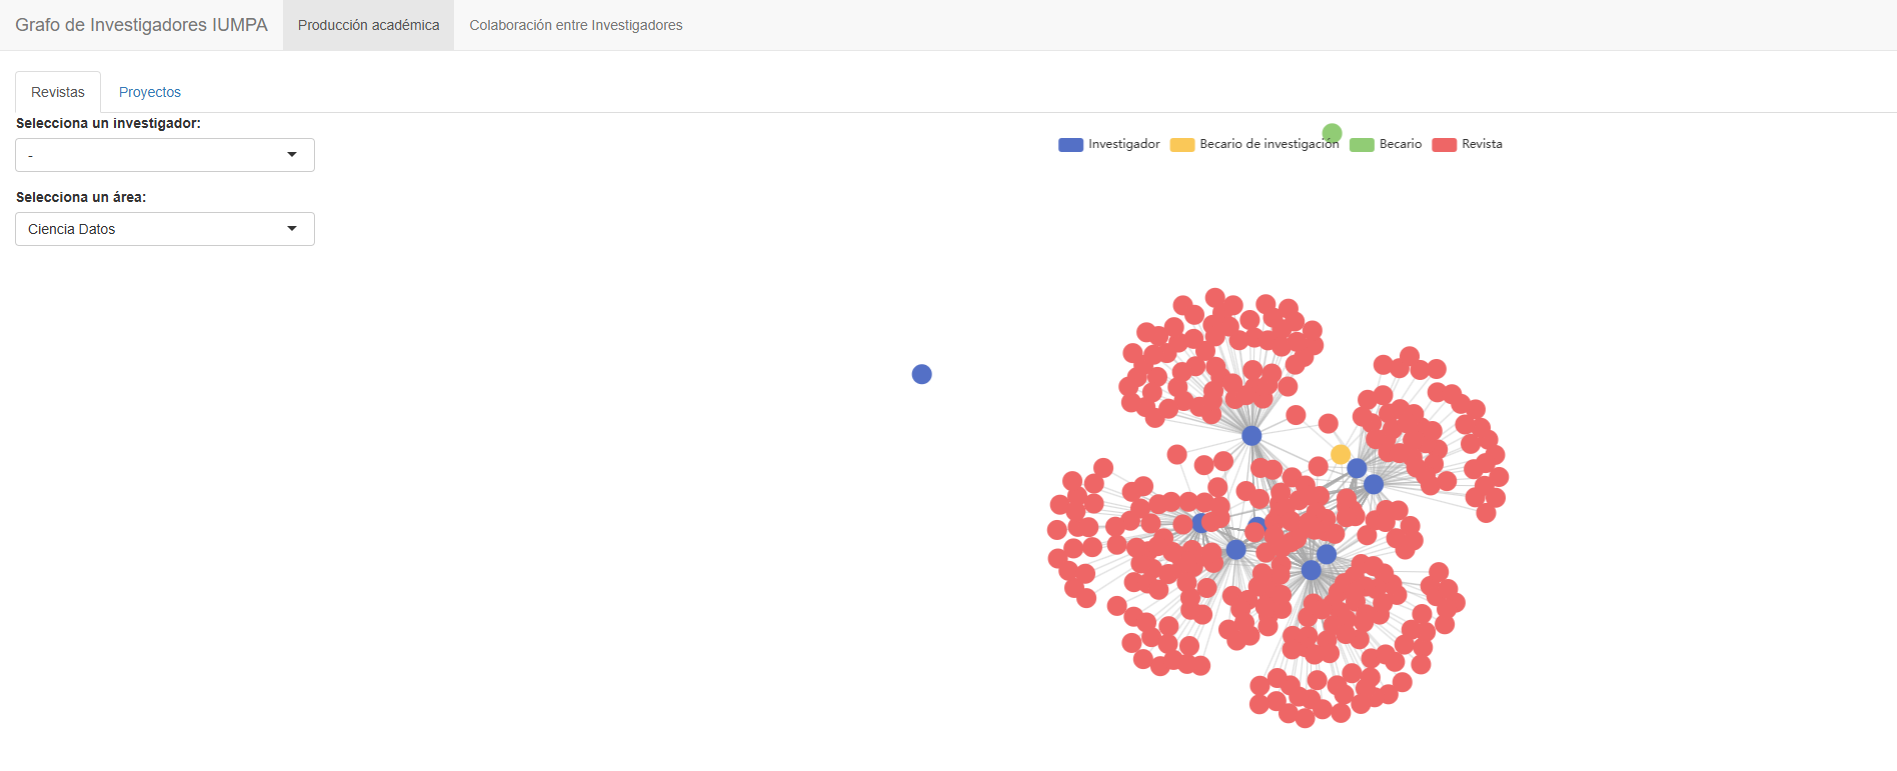
\includegraphics[width=0.48\textwidth]{imgs/filtrado_area.png}
\caption{Ejemplos de filtrado mediante selectores en los grafos interactivos.}
\label{fig:filtros_selectores}
\end{figure}

Además de estos selectores, la leyenda de los grafos también actuaba como un elemento interactivo. Al seleccionar o deseleccionar una categoría de la leyenda, la aplicación permitía ocultar o mostrar los nodos pertenecientes a dicho grupo. Esta funcionalidad resultaba útil para centrar la visualización en determinados tipos de elementos, por ejemplo ocultando algún tipo de personal cuando se quería observar con mayor claridad una parte concreta del grafo.

\begin{figure}[H]
\centering
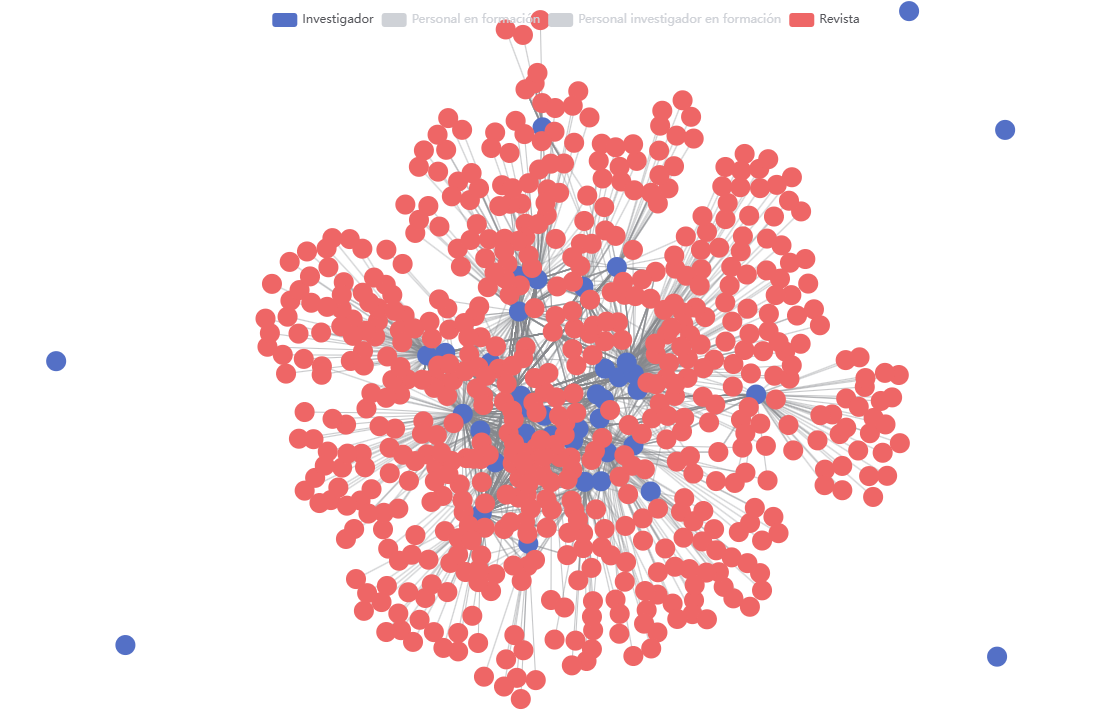
\includegraphics[width=0.95\textwidth]{imgs/filtrado_leyenda.png}
\caption{Ejemplo de filtrado visual mediante la selección de categorías en la leyenda del grafo.}
\label{fig:filtro_leyenda}
\end{figure}

La aplicación también utilizó recursos de codificación visual para facilitar la interpretación de los grafos. En primer lugar, se emplearon colores fijos para diferenciar los tipos de elementos representados. En todos los grafos, los investigadores se muestran en azul, los becarios en verde y los becarios de investigación en amarillo. Además, en los grafos de producción académica, las revistas y los proyectos se representan en rojo. Esta codificación cromática se mantuvo constante entre vistas para que el usuario pudiera interpretar los nodos de forma homogénea al cambiar de grafo.

Junto con el color, en los grafos de colaboración entre investigadores se incorporó una diferencia de tamaño entre nodos. En estas visualizaciones, el tamaño del nodo representaba el número de conexiones del investigador dentro del grafo correspondiente. Por tanto, los nodos de mayor tamaño indicaban investigadores con más conexiones dentro de la red mostrada en cada caso (colaboraciones derivadas de artículos compartidos en un grafo y colaboraciones derivadas de proyectos comunes en el otro). Esta representación añadía una segunda capa de información visual y permitía identificar nodos con mayor conectividad dentro de la red, sin plantear esta información como una métrica individual de productividad.

Además de estos elementos visuales, la exploración de los grafos se apoyó en mecanismos de interacción directa. Al situar el cursor sobre un nodo, la aplicación mostraba información emergente asociada al elemento seleccionado, con diferentes resultados según el grafo: 
\begin{itemize}
    \item \textbf{Investigadores y revistas}: esta información incluía, para los investigadores, el número de revistas asociadas y el número de artículos recopilados, mientras que para las revistas indicaba el número de investigadores vinculados a ellas.

    \item \textbf{Investigadores y proyectos}: la información emergente mostraba, para cada investigador, el número de proyectos asociados y, para cada proyecto, el número de investigadores vinculados.

    \item \textbf{Colaboración entre investigadores}: en ambos casos, esta información permitía consultar el número total de conexiones del investigador dentro de la red mostrada.
\end{itemize}

Asimismo, la interacción con los enlaces permitía interpretar qué elementos quedaban conectados en el grafo, reforzando la lectura de las relaciones visualizadas.

Por otro lado, la selección mediante clic permitía pasar de esta identificación rápida a una consulta más detallada. Al seleccionar un nodo, la aplicación mostraba información específica del elemento seleccionado en un panel informativo, adaptada al tipo de entidad consultada. En los grafos de producción académica, este panel ofrecía distinta información según el tipo de nodo:

\begin{itemize}
    \item \textbf{Investigadores}: se mostraba su nombre y, según el grafo consultado, los artículos publicados o los proyectos en los que había participado.

    \item \textbf{Revistas}: se presentaba el nombre de la revista, la editorial asociada cuando estaba disponible y los artículos junto con los investigadores correspondientes.

    \item \textbf{Proyectos}: se recogía el nombre del proyecto y los investigadores que habían participado en él, diferenciando entre investigadores principales y no principales cuando dicha información estaba disponible.
\end{itemize}

En los grafos de colaboración entre investigadores, el panel mostraba la lista de investigadores del IUMPA con los que el nodo seleccionado había trabajado.

\begin{figure}[H]
\centering

\begin{minipage}{0.48\textwidth}
\centering
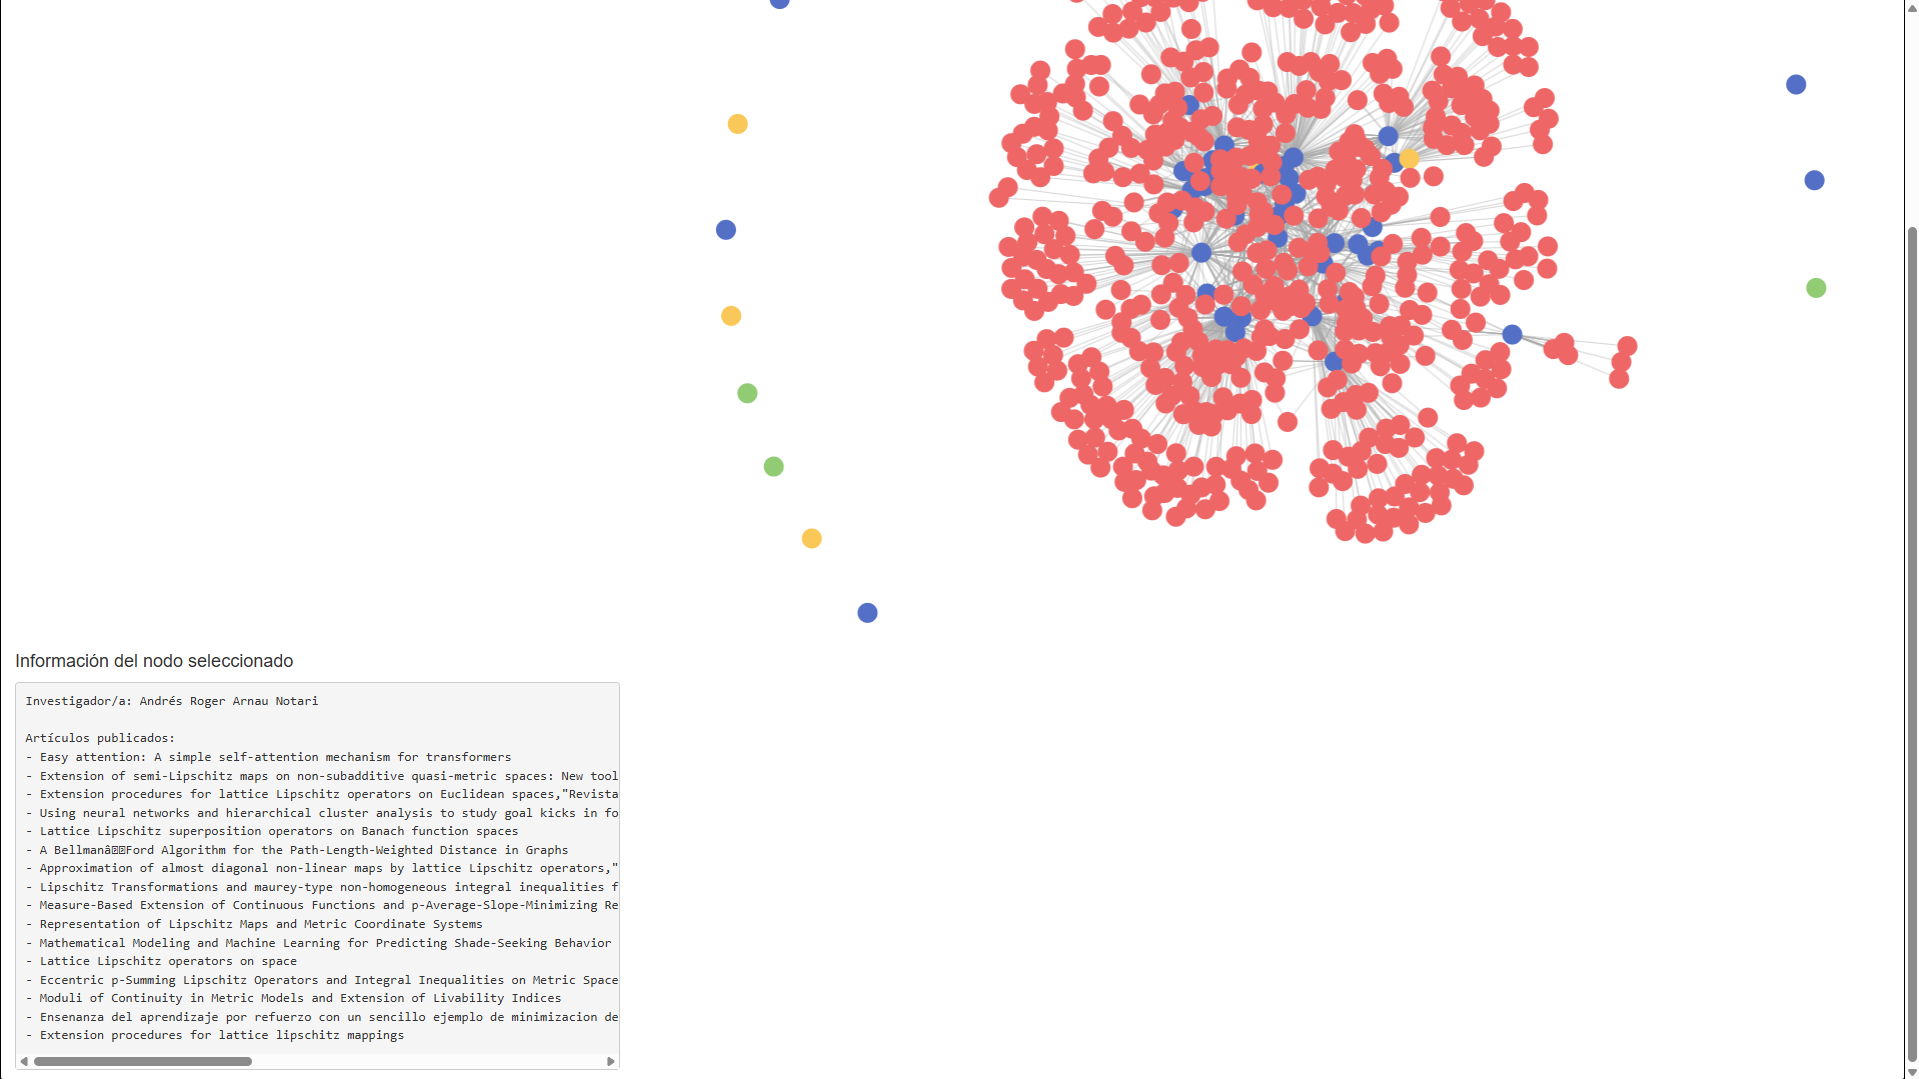
\includegraphics[width=\textwidth]{imgs/panel_investigador_revistas.png}
\end{minipage}
\hfill
\begin{minipage}{0.48\textwidth}
\centering
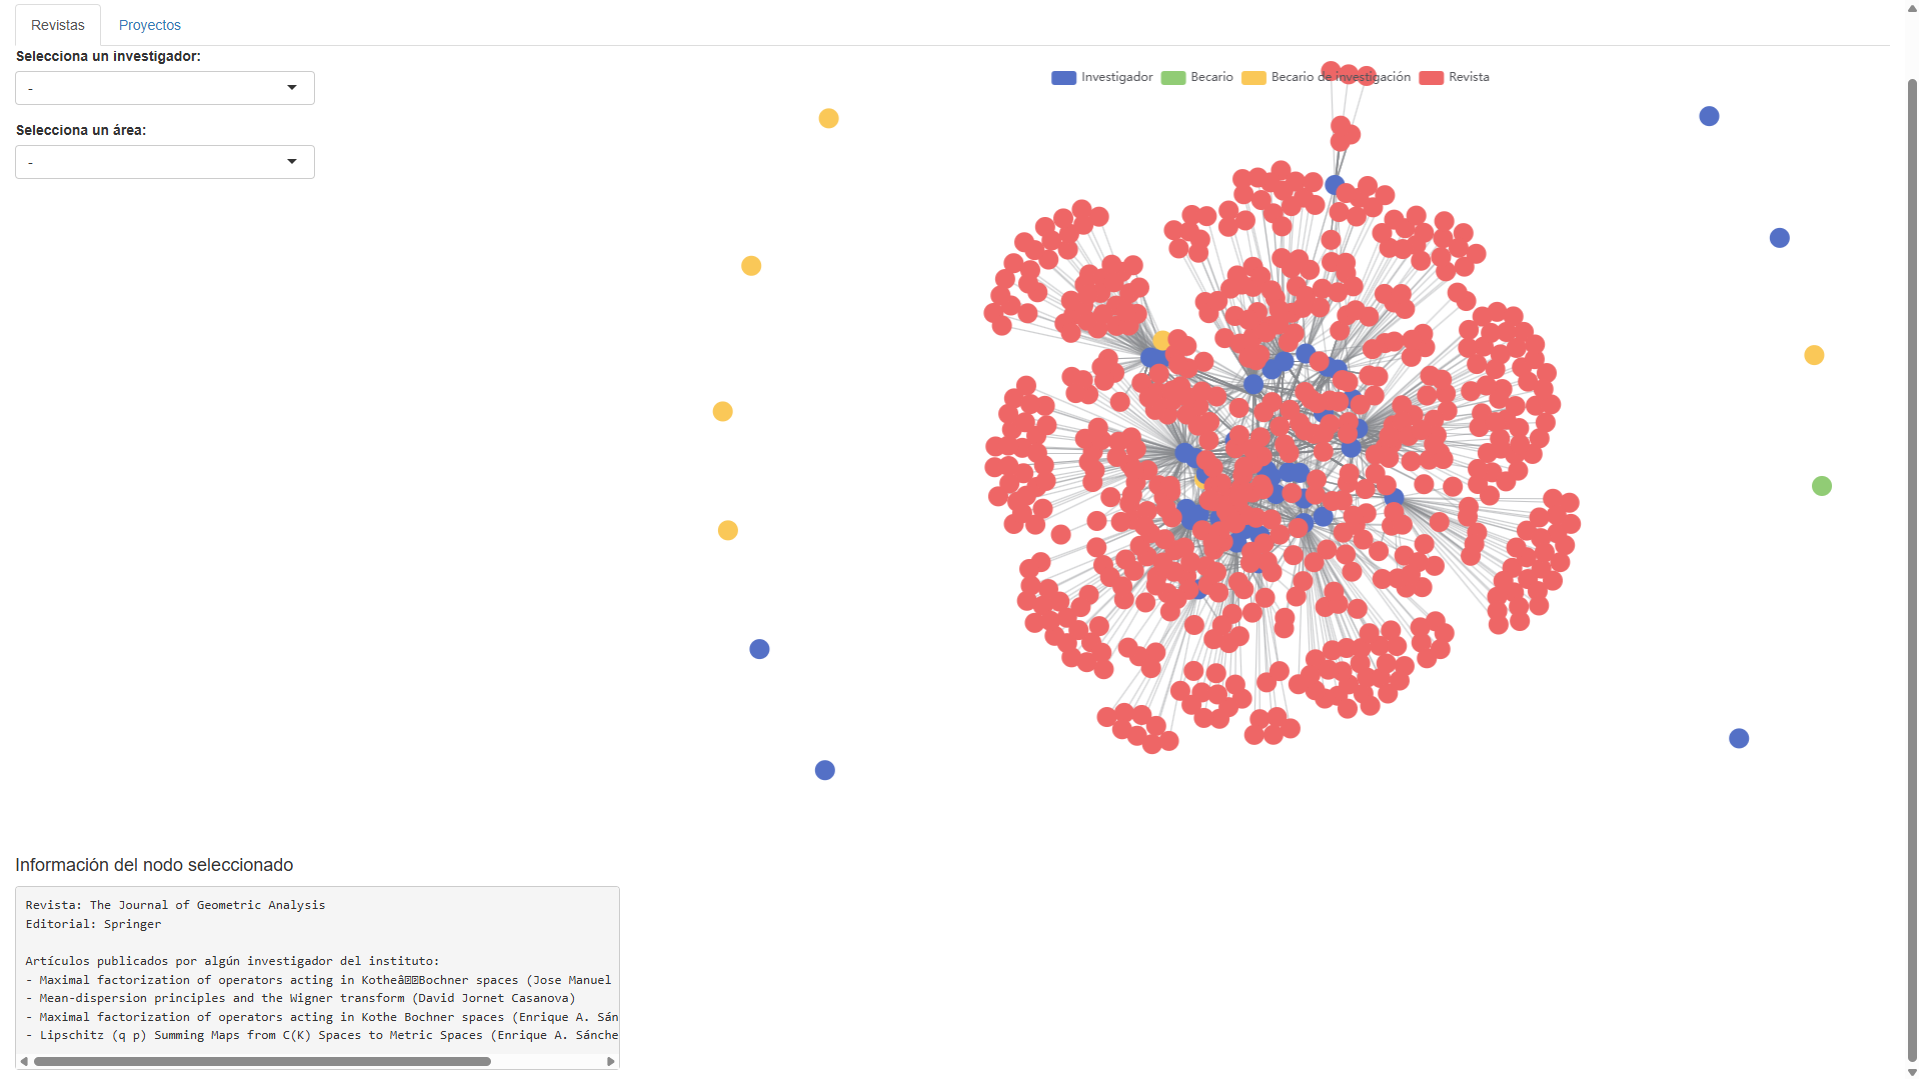
\includegraphics[width=\textwidth]{imgs/panel_revista.png}
\end{minipage}

\vspace{0.6em}

\begin{minipage}{0.48\textwidth}
\centering
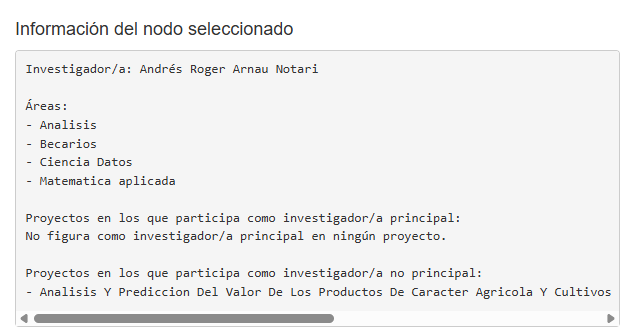
\includegraphics[width=\textwidth]{imgs/panel_investigador_proyectos.png}
\end{minipage}
\hfill
\begin{minipage}{0.48\textwidth}
\centering
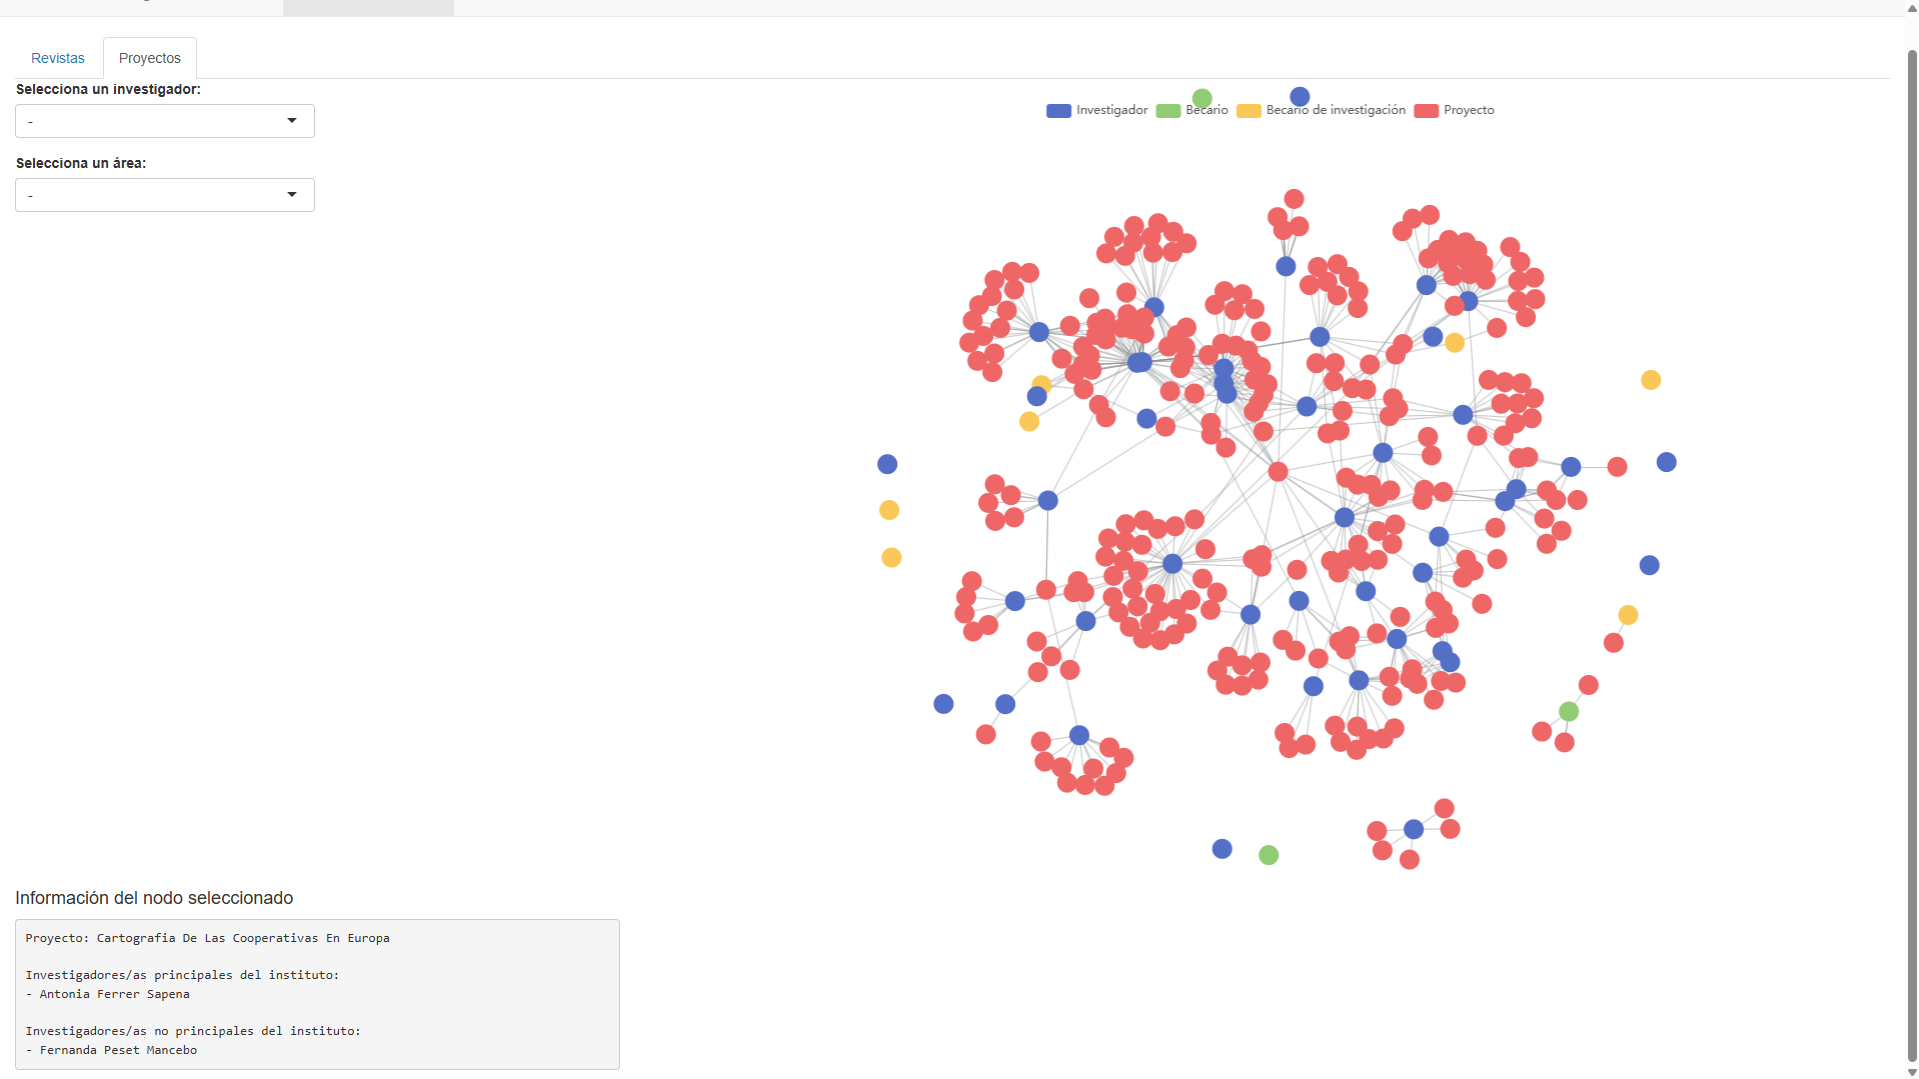
\includegraphics[width=\textwidth]{imgs/panel_proyecto.png}
\end{minipage}

\caption{Ejemplos de información mostrada al seleccionar distintos tipos de nodo en los grafos de producción académica.}
\label{fig:paneles_informativos}
\end{figure}

En conclusión, estos elementos permitían complementar la visualización global de los grafos con mecanismos de exploración más detallados. El usuario podía partir de una vista general de las relaciones y, posteriormente, aplicar filtros, ocultar categorías, consultar información emergente o seleccionar nodos concretos para acceder a los datos asociados.

\section{Valoración de la aplicación desarrollada}

La aplicación desarrollada permitió explotar la base de datos construida desde una perspectiva visual e interactiva. Su principal aportación fue transformar los ficheros tabulares en grafos explorables, facilitando la consulta de relaciones entre investigadores, revistas y proyectos, así como de las colaboraciones derivadas de publicaciones y proyectos compartidos. De este modo, la herramienta actuó como una capa de consulta sobre la base de datos, haciendo más accesible una información que en formato tabular resultaría menos inmediata.

La separación de la información en varias vistas resultó adecuada para evitar una única red excesivamente compleja. Los grafos de producción académica permitieron consultar relaciones entre investigadores y revistas o proyectos, mientras que los grafos de colaboración ofrecieron una perspectiva centrada en las relaciones entre miembros del instituto. Además, los elementos de interacción incorporados permitieron reducir la complejidad visual mediante filtros y acceder a información concreta mediante selección de nodos.

No obstante, la aplicación debe entenderse como una herramienta exploratoria condicionada por los datos disponibles. Algunos grafos pueden resultar densos en las vistas generales y la posición de los nodos debe interpretarse como un recurso visual, no como una medida analítica. Asimismo, la información mostrada depende de la completitud de las fuentes consultadas, por lo que la ausencia de una relación o registro no implica necesariamente su inexistencia. Aun así, la herramienta cumple su función principal dentro del proyecto, al facilitar la exploración visual de la actividad investigadora del IUMPA y servir como base para futuras ampliaciones.

%%%%%%%%%%%%%%%%%%%%%%%%%%%%%%%%%%%%%%%%%%%%%%%%%%%%%%%%%%%%%%%%%%%%%%%%%%%%%%%

%%%%%%%%%%%
%Capítulo 6
%%%%%%%%%%%

\chapter{Agrupación semántica de investigadores}

\textit{BORRAR Este capítulo describirá la ampliación analítica del proyecto, orientada a estudiar afinidades temáticas entre investigadores a partir de las revistas en las que han publicado. Para ello, se explicará el proceso de obtención de palabras clave representativas, la construcción de representaciones temáticas de los investigadores y la aplicación de distintos modelos de clustering y reducción de dimensionalidad. El objetivo será mostrar el proceso metodológico seguido hasta obtener una agrupación semántica interpretable.}

Tras la construcción de la base de datos y el desarrollo de los grafos interactivos, el proyecto ya permitía explorar la actividad investigadora del IUMPA desde una perspectiva relacional. Sobre esta base, se planteó estudiar si los datos recopilados podían revelar afinidades temáticas entre investigadores más allá de las colaboraciones y publicaciones observables. Para ello, se propuso una ampliación analítica basada en las revistas en las que publica cada investigador, partiendo de la idea de que dichas revistas pueden aportar información sobre sus áreas de interés al estar asociadas a diferentes campos.

A partir de esta hipótesis, se utilizaron palabras clave representativas de las revistas para construir perfiles temáticos de los investigadores y aplicar distintos métodos de agrupamiento orientados a identificar posibles grupos con intereses próximos.

El propósito de este análisis no fue obtener una clasificación cerrada de los miembros del instituto, sino explorar hasta qué punto la información disponible permitía detectar agrupaciones interpretables desde un punto de vista semántico. Por ello, el proceso combinó varias representaciones de los datos, distintos modelos de clustering y técnicas de reducción de dimensionalidad, valorando los resultados tanto mediante métricas cuantitativas como mediante su coherencia temática.

\section{Preparación del vocabulario temático}

Hasta este punto, las revistas habían servido principalmente para describir la actividad bibliográfica de los investigadores y construir relaciones dentro de la base de datos. En esta fase, esas mismas revistas comenzaron a tener la función adicional de actuar como indicadores temáticos. Para ello, se utilizaron las palabras clave asociadas a cada revista como forma de aproximar los campos con los que estaban relacionadas.

El objetivo no era describir cada revista exhaustivamente, sino disponer de un vocabulario suficientemente representativo para caracterizar su orientación temática. Esta decisión permitía trabajar con la revista como unidad intermedia entre el artículo individual y el investigador. De este modo, las palabras clave no se utilizaron para analizar el contenido detallado de cada publicación, sino para construir una aproximación general al tipo de temas presentes en los medios donde habían publicado los investigadores.

Una vez recopiladas las palabras clave, fue necesario revisar el conjunto global de términos antes de utilizarlo en los modelos de agrupamiento. Algunas palabras aparecían asociadas a un gran número de revistas y, por tanto, aportaban poca capacidad diferenciadora. Otras, en cambio, eran demasiado específicas, lo que dificultaba la identificación de patrones compartidos entre investigadores. Por ello, la selección final buscó un equilibrio entre representatividad y utilidad para comparar perfiles temáticos.

Además de esta depuración, se revisó manualmente la coherencia del vocabulario para reducir duplicidades y unificar variantes muy próximas. Con ello se buscó que términos muy relacionados quedaran representados de forma consistente, evitando una fragmentación innecesaria del vocabulario. En consecuencia, las palabras clave no se emplearon como una recopilación directa de términos aislados, sino como un conjunto revisado y preparado para servir de base al análisis semántico.

Durante la revisión posterior de los primeros resultados se observó que no todos los términos del vocabulario contribuían del mismo modo a caracterizar intereses científicos. En particular, algunas palabras hacían referencia a localizaciones geográficas u otros elementos contextuales que podían aparecer vinculados a determinadas revistas, pero que no describían propiamente una línea de investigación. Aunque estos términos formaban parte de la información recopilada, su presencia podía desplazar la agrupación hacia coincidencias poco relevantes desde el punto de vista temático.

Por este motivo, se realizó una depuración adicional del vocabulario antes de consolidar la base final utilizada en el análisis. Esta revisión permitió eliminar términos que podían introducir ruido en la comparación entre investigadores y centrar la representación en palabras con mayor capacidad para describir ámbitos científicos. De esta forma, la selección final no solo buscó reducir términos poco informativos, sino también asegurar que el vocabulario empleado reflejara afinidades temáticas reales y no relaciones espurias derivadas de elementos accesorios.

Con este proceso quedó definida una base temática de revistas y palabras clave depuradas, preparada para trasladar posteriormente la información desde las revistas hacia los perfiles de los investigadores.

\section{Representación temática de los investigadores}

La base temática disponible relacionaba cada revista con un conjunto de palabras clave, pero el objetivo del análisis era comparar perfiles de investigadores. Por ello, el siguiente paso consistió en trasladar esa información desde las revistas hacia los investigadores, construyendo una representación en la que cada persona quedara descrita a partir de los términos asociados a las revistas en las que había publicado.

Para realizar esta transformación, se combinaron dos estructuras ya disponibles. La primera recogía la relación entre investigadores y revistas en las que habían publicado, mientras que la segunda asociaba cada revista con un conjunto de palabras clave. Al unir ambas estructuras, las palabras clave de cada revista pasaban a formar parte del perfil del investigador que había publicado en ella.

De este modo, no se asignaban palabras clave directamente a los investigadores, sino a través de las revistas que conectaban su actividad bibliográfica con determinados ámbitos temáticos. Esta decisión permitía conservar una trazabilidad clara entre los tres elementos implicados, es decir, investigador, revista y palabra clave. Así, además de saber qué términos caracterizaban a cada investigador, era posible identificar de qué revistas procedían, lo que facilitaba la interpretación posterior de los resultados.

A partir de esta información se construyó una primera matriz de representación basada en presencia y ausencia de términos. En esta matriz, cada fila correspondía a un investigador y cada columna a una palabra clave del vocabulario temático. El valor de cada celda indicaba si una determinada palabra estaba asociada o no al investigador correspondiente:

\[
M_{ij} =
\begin{cases}
1, & \text{si la palabra clave } j \text{ está asociada al investigador } i,\\
0, & \text{en caso contrario.}
\end{cases}
\]

Con esta estructura, la información textual quedaba transformada en un formato numérico sencillo, adecuado para calcular distancias entre perfiles y aplicar métodos de agrupamiento. Su interpretación también resultaba directa, ya que cada investigador quedaba descrito por el conjunto de términos asociados a las revistas en las que había publicado.

El proceso seguido para transformar las revistas publicadas en perfiles temáticos comparables se resume en la Figura~\ref{fig:flujo_representacion_tematica}.

\begin{figure}[H]
\centering
\small
\fbox{
\begin{minipage}{0.82\textwidth}
\centering
Revistas en las que ha publicado cada investigador

\vspace{0.2cm}
$\downarrow$

\vspace{0.2cm}
Palabras clave asociadas a esas revistas

\vspace{0.2cm}
$\downarrow$

\vspace{0.2cm}
Asignación de palabras clave al investigador

\vspace{0.2cm}
$\downarrow$

\vspace{0.2cm}
Perfil temático del investigador

\vspace{0.2cm}
$\downarrow$

\vspace{0.2cm}
Representación matricial de los perfiles

\vspace{0.2cm}
$\downarrow$

\vspace{0.2cm}
Entrada para los modelos de agrupamiento
\end{minipage}
}
\caption{Proceso de construcción de perfiles temáticos a partir de las revistas publicadas por los investigadores.}
\label{fig:flujo_representacion_tematica}
\end{figure}

La matriz binaria ofrecía una primera representación sencilla e interpretable de los perfiles temáticos. A partir de ella se realizaron distintas pruebas de agrupamiento, aplicando diferentes formas de comparar los perfiles de los investigadores. Sin embargo, los resultados obtenidos no mostraron una separación suficientemente clara entre grupos. Las métricas de evaluación, con valores bajos del índice de Silhouette en las mejores pruebas iniciales, indicaban que las agrupaciones generadas no eran lo bastante consistentes. Por ello, se decidió no forzar una interpretación de estos primeros resultados y revisar la forma en que estaban representados los perfiles temáticos.

El principal problema de este enfoque era que la similitud entre investigadores dependía de coincidencias literales entre términos. Por ello, dos perfiles próximos desde un punto de vista conceptual podían aparecer como poco similares si las revistas asociadas a cada uno estaban descritas mediante vocabularios distintos. Esta situación resultaba especialmente relevante en un contexto como el del IUMPA, donde pueden existir líneas de trabajo cercanas expresadas con términos parcialmente diferentes.

Para tratar de mejorar esta situación, y antes de pasar al enfoque semántico, se introdujo una ponderación sobre la matriz inicial. El objetivo era evitar que todas las palabras clave tuvieran el mismo peso dentro de la comparación entre investigadores. En particular, se buscaba reducir la influencia de términos excesivamente comunes, que podían aparecer en muchos perfiles y aportar poca capacidad diferenciadora, así como de palabras demasiado raras, cuya aparición aislada podía condicionar de forma desproporcionada los resultados.

La ponderación aplicada consistió en una penalización simétrica basada en una función gaussiana. En este enfoque, el peso de cada palabra clave dependía de su frecuencia respecto a la frecuencia media del vocabulario. Las palabras con frecuencias intermedias recibían mayor peso, al considerarse potencialmente más representativas para comparar perfiles, mientras que los términos demasiado frecuentes o demasiado aislados quedaban penalizados. El peso de una palabra clave \(j\) se definió como:

\[
w_j = e^{-\frac{(f_j - \mu)^2}{2\sigma^2}}
\]

donde \(f_j\) representa la frecuencia de la palabra clave \(j\), \(\mu\) la frecuencia media de las palabras clave y \(\sigma\) un parámetro que controla el grado de penalización aplicado a los términos situados en los extremos de la distribución de frecuencias.

La estrategia permitió incorporar una primera forma de discriminación dentro de la representación. No obstante, aunque la ponderación mejoraba conceptualmente la matriz binaria, los resultados siguieron sin ofrecer una separación numéricamente satisfactoria entre grupos. La comparación continuaba dependiendo de la presencia explícita de los términos en el vocabulario, por lo que no resolvía la limitación principal del enfoque basado en coincidencias literales.

A partir de esta evaluación, se decidió pasar a una representación más flexible mediante \textit{word embeddings}. En lugar de tratar cada palabra clave como una etiqueta independiente, este enfoque representa los términos mediante vectores numéricos situados en un espacio semántico. En este caso se utilizó la librería \textit{sentence-transformers}, basada en el enfoque Sentence-BERT~\cite{sentencebert}, junto con el modelo multilingüe \textit{paraphrase-multilingual-MiniLM-L12-v2}, que transforma cada término en un vector denso de 384 dimensiones~\cite{minilm_multilingual}. De este modo, dos palabras distintas pueden aparecer próximas en dicho espacio si están relacionadas conceptualmente, aunque no coincidan de forma literal.

Esta propiedad resultaba útil para el objetivo del análisis, ya que permitía comparar perfiles de investigadores no solo a partir de las palabras exactas que compartían, sino también considerando la relación conceptual entre los términos que caracterizaban sus revistas. Así, la representación dejaba de depender exclusivamente de coincidencias textuales y pasaba a incorporar una noción de proximidad conceptual entre palabras clave.

Para construir el perfil semántico de cada investigador, se obtuvieron los vectores correspondientes a sus palabras clave y se calculó una representación agregada a partir de ellos. Formalmente, si \(K_i\) representa el conjunto de palabras clave asociadas al investigador \(i\), y \(\mathbf{e}(w)\) representa el vector semántico de una palabra \(w\), el perfil del investigador puede expresarse como:

\[
\mathbf{v}_i = \frac{1}{|K_i|}\sum_{w \in K_i} \mathbf{e}(w)
\]

De esta forma, cada investigador dejó de estar representado únicamente por una lista de términos o por una fila de una matriz binaria, y pasó a estar descrito mediante un vector continuo que resumía, de forma aproximada, el contenido semántico de su perfil temático.

Esta transformación permitió trabajar con una representación más flexible de los investigadores. Mientras que la matriz binaria resultaba útil como primera aproximación interpretable, los embeddings incorporaban una dimensión semántica que permitía comparar perfiles más allá de la coincidencia exacta de palabras clave, recogiendo afinidades entre términos conceptualmente próximos.

\section{Modelos de clustering}

\textit{BORRAR Este apartado presentará los distintos modelos de agrupación aplicados sobre las representaciones temáticas construidas. Se describirán las pruebas realizadas con diferentes medidas de distancia, métodos de clustering y técnicas de reducción de dimensionalidad, así como los criterios utilizados para comparar sus resultados. El apartado también recogerá las dificultades encontradas durante el proceso experimental y las decisiones metodológicas adoptadas para seleccionar las configuraciones más adecuadas.}

Una vez construidas las representaciones temáticas de los investigadores, el siguiente paso consistió en estudiar si esas representaciones permitían identificar grupos de perfiles próximos. Al no existir una clasificación previa que actuara como variable objetivo, el problema se planteó como una tarea de aprendizaje no supervisado. El propósito no era asignar a cada investigador una etiqueta predefinida, sino explorar si los datos contenían una estructura latente capaz de agrupar perfiles con afinidades temáticas.

El proceso de agrupamiento se abordó de forma experimental. Para ello, se probaron distintas configuraciones a partir de las representaciones descritas anteriormente. En primer lugar, se trabajó con la matriz binaria de presencia y ausencia de palabras clave, así como con su versión ponderada mediante la penalización gaussiana. Posteriormente, el análisis se trasladó a las representaciones semánticas obtenidas mediante \textit{word embeddings}, con el objetivo de comparar perfiles no solo por las palabras exactas que compartían, sino también por la proximidad conceptual entre los términos que los caracterizaban.

En esta fase se evitó incorporar directamente las áreas de trabajo de los investigadores como variables del modelo. Aunque esta información podía resultar útil para interpretar los grupos obtenidos, incluirla en la construcción de los perfiles habría condicionado el agrupamiento hacia una clasificación ya existente. Por ello, los modelos se basaron únicamente en la información derivada de las revistas y de sus palabras clave, permitiendo comprobar si las afinidades temáticas emergían a partir de los datos bibliográficos recopilados.

Cada configuración quedaba determinada por varios elementos: la representación de entrada, la medida de distancia o similitud utilizada, el método de agrupamiento y, en algunos casos, la aplicación previa de una técnica de reducción de dimensionalidad. La Tabla~\ref{tab:elementos_clustering} resume los principales componentes considerados durante el proceso experimental.

\begin{table}[H]
\centering
\small
\begin{tabular}{p{0.25\textwidth} p{0.34\textwidth} p{0.31\textwidth}}
\hline
\textbf{Elemento} & \textbf{Opciones consideradas} & \textbf{Función dentro del análisis} \\
\hline
Representación de entrada & Matriz binaria, matriz ponderada y embeddings semánticos & Definir cómo se describe temáticamente cada investigador \\
\hline
Medidas de proximidad & Distancias o similitudes adecuadas al tipo de representación, como Jaccard, Hamming, correlación, coseno, euclídea o Manhattan & Cuantificar la proximidad entre perfiles de investigadores \\
Medidas de proximidad & Distancias o similitudes seleccionadas según el tipo de representación utilizada & Cuantificar la proximidad entre perfiles de investigadores \\
\hline
Método de agrupamiento & Clustering jerárquico con diferentes particiones del árbol de agrupamiento & Formar grupos de investigadores con perfiles temáticos próximos \\
\hline
Reducción de dimensionalidad & UMAP aplicado sobre las representaciones semánticas & Proyectar los perfiles en un espacio de menor dimensión y comparar la estructura obtenida \\
\hline
Evaluación & Índice de Silhouette y revisión temática de los grupos & Comparar configuraciones y valorar la coherencia de las agrupaciones \\
\hline
\end{tabular}
\caption{Elementos considerados en el proceso de agrupamiento temático.}
\label{tab:elementos_clustering}
\end{table}

La elección de la medida de proximidad dependía del tipo de representación utilizada. En las matrices binarias o ponderadas, la comparación se basaba en el grado de coincidencia o diferencia entre los términos asociados a cada investigador. En las representaciones mediante embeddings, las distancias se calculaban sobre vectores continuos que resumían el perfil semántico de cada persona. Esta diferencia era importante, ya que no todas las medidas resultaban igual de adecuadas para todos los tipos de datos.

El método de agrupamiento se centró principalmente en el clustering jerárquico. Este enfoque resultaba adecuado para el carácter exploratorio del análisis, ya que permite observar cómo los investigadores se van agrupando progresivamente en función de su proximidad. Además, no obliga a asumir desde el principio una estructura rígida de los datos, sino que permite estudiar distintas particiones a partir del mismo proceso de agrupamiento. De este modo, se podían comparar soluciones con diferente número de grupos y valorar cuáles ofrecían una separación más clara y una interpretación temática más coherente.

Junto a los modelos aplicados directamente sobre las representaciones originales, se incorporó también una fase de reducción de dimensionalidad. En particular, se utilizó UMAP, una técnica diseñada para proyectar datos de alta dimensión en espacios de menor dimensión preservando, en la medida de lo posible, relaciones de proximidad entre observaciones~\cite{umap}. Su uso permitía estudiar si una representación más compacta de los perfiles semánticos facilitaba la formación de grupos más diferenciados y comparables.

La evaluación de las configuraciones no se basó únicamente en la inspección visual de los grupos. Para disponer de una medida cuantitativa se utilizó el índice de Silhouette~\cite{rousseeuw}, que permite valorar hasta qué punto cada observación está mejor asignada a su propio grupo que a grupos alternativos. Para un investigador \(i\), este índice puede expresarse como:

\[
s(i) = \frac{b(i) - a(i)}{\max\{a(i), b(i)\}}
\]

donde \(a(i)\) representa la distancia media entre el investigador \(i\) y el resto de elementos de su mismo grupo, mientras que \(b(i)\) representa la menor distancia media entre \(i\) y los elementos de otro grupo. Valores próximos a 1 indican una asignación bien separada, valores cercanos a 0 reflejan grupos poco diferenciados y valores negativos sugieren que la observación podría estar más próxima a otro grupo.

No obstante, la selección de configuraciones no se realizó de forma automática a partir de una única métrica. Dado que el objetivo era obtener agrupaciones interpretables desde el punto de vista temático, los valores del índice de Silhouette se complementaron con una revisión cualitativa de los grupos generados. Esta revisión consideraba aspectos como el tamaño de los grupos, la coherencia de las palabras clave asociadas a cada uno y la plausibilidad temática de las agrupaciones resultantes.

El proceso experimental mostró que la representación de entrada tenía un papel determinante en la calidad de los agrupamientos. Las configuraciones basadas en coincidencias literales permitieron establecer una primera referencia, pero también evidenciaron las limitaciones de trabajar únicamente con presencia o ponderación de palabras clave. Por ello, las configuraciones basadas en embeddings y aquellas combinadas con reducción de dimensionalidad adquirieron un papel central en la búsqueda de agrupaciones más coherentes e interpretables.

\section{Evaluación y discusión de los resultados}

\textit{Este apartado evaluará los resultados obtenidos en la fase de agrupación semántica de investigadores. Se analizarán las diferencias entre los enfoques probados, la utilidad de las representaciones semánticas frente a las coincidencias literales de palabras clave y la calidad de las agrupaciones obtenidas a partir de métricas cuantitativas y criterios de coherencia temática. También se discutirá hasta qué punto estos resultados complementan la información relacional proporcionada por los grafos y qué limitaciones deben tenerse en cuenta al interpretar los grupos identificados.}

%%%%%%%%%%%%%%%%%%%%%%%%%%%%%%%%%%%%%%%%%%%%%%%%%%%%%%%%%%%%%%%%%%%%%%%%%%%%%%%
%                               BLOQUE III: cierre                            %
%%%%%%%%%%%%%%%%%%%%%%%%%%%%%%%%%%%%%%%%%%%%%%%%%%%%%%%%%%%%%%%%%%%%%%%%%%%%%%%

%%%%%%%%%%%
%Capítulo 7
%%%%%%%%%%%

\chapter{Conclusiones y trabajo futuro}

\textit{Este capítulo recogerá las conclusiones generales del trabajo a partir del desarrollo y las valoraciones realizadas en los capítulos anteriores. Se sintetizarán los principales resultados alcanzados en relación con la construcción de la base de datos, el desarrollo de la aplicación interactiva y la agrupación semántica de investigadores, evitando introducir información nueva que no haya sido discutida previamente.}

\textit{También se valorará el grado de cumplimiento de los objetivos planteados al inicio del trabajo y se destacarán las principales aportaciones del proyecto desde el punto de vista de la ciencia de datos. Finalmente, se señalarán las limitaciones generales que permanecen y se propondrán posibles líneas de trabajo futuro, como la ampliación o actualización de las fuentes de datos, la mejora de la aplicación interactiva y la extensión de la parte analítica.}

\section{Conclusiones generales}

\textit{Este apartado sintetizará las conclusiones principales del trabajo a partir de los resultados y valoraciones expuestos en los capítulos anteriores. Se recogerá de forma global qué ha aportado la construcción de la base de datos, qué utilidad tiene la aplicación interactiva desarrollada y qué valor añade la agrupación semántica de investigadores. El objetivo será ofrecer una visión conjunta del proyecto, destacando su contribución a la comprensión de la actividad investigadora del IUMPA sin introducir resultados nuevos.}

\section{Cumplimiento de los objetivos}

\textit{Este apartado revisará los objetivos planteados al inicio de la memoria y valorará en qué medida han sido alcanzados. Se relacionarán los objetivos específicos con las fases desarrolladas durante el proyecto: identificación de entidades y relaciones, recopilación y depuración de datos, construcción de la base de datos, desarrollo de la aplicación interactiva y análisis de afinidades temáticas. Esta sección permitirá cerrar el trabajo de forma coherente, conectando lo propuesto en la introducción con los resultados obtenidos.}

\section{Líneas de trabajo futuro}

\textit{Este apartado planteará posibles ampliaciones y mejoras del proyecto. Se incluirán líneas como la incorporación de nuevas fuentes de datos, la actualización periódica de la base, la mejora de la aplicación interactiva, la ampliación de las funcionalidades de visualización y el perfeccionamiento de la parte analítica. También se podrán mencionar posibles extensiones metodológicas, como nuevas formas de representación semántica, métricas adicionales o procedimientos más automatizados de validación y actualización de datos.}

\textit{Una idea: Contar cuántas veces aparece una palabra para cada investigador en las asociaciones temáticas, en lugar de solo si aparece o no, para saber cuánto de importante es un término/concepto para cada investigador.}

\section{Legado}

\section{Relación del TFG con GCD}

%%%%%%%%%%%%%%%%%%%%%%%%%%%%%%%%%%%%%%%%%%%%%%%%%%%%%%%%%%%%%%%%%%%%%%%%%%%%%%%
%                                BIBLIOGRAFIA                                 %
%%%%%%%%%%%%%%%%%%%%%%%%%%%%%%%%%%%%%%%%%%%%%%%%%%%%%%%%%%%%%%%%%%%%%%%%%%%%%%%

\begin{thebibliography}{99}

\bibitem{newmannetworks}
Newman, M. E. J.
\newblock \textit{Networks: An Introduction}.
\newblock Oxford University Press, 2010.

\bibitem{manning}
Manning, C. D., Raghavan, P. y Schütze, H.
\newblock \textit{Introduction to Information Retrieval}.
\newblock Cambridge University Press, 2008.

\bibitem{hastie}
Hastie, T., Tibshirani, R. y Friedman, J.
\newblock \textit{The Elements of Statistical Learning}.
\newblock Springer, 2009.

\bibitem{mikolov}
Mikolov, T., Chen, K., Corrado, G. y Dean, J.
\newblock Efficient Estimation of Word Representations in Vector Space.
\newblock \textit{arXiv preprint arXiv:1301.3781}, 2013.

\bibitem{RGPD2016}
Parlamento Europeo y Consejo de la Unión Europea.
\newblock \textit{Reglamento (UE) 2016/679 del Parlamento Europeo y del Consejo, de 27 de abril de 2016, relativo a la protección de las personas físicas en lo que respecta al tratamiento de datos personales y a la libre circulación de estos datos}.
\newblock Diario Oficial de la Unión Europea, 2016.

\bibitem{LOPDGDD2018}
Jefatura del Estado.
\newblock \textit{Ley Orgánica 3/2018, de 5 de diciembre, de Protección de Datos Personales y garantía de los derechos digitales}.
\newblock Boletín Oficial del Estado, núm. 294, 2018.

\bibitem{web_iumpa}
Instituto Universitario de Matemática Pura y Aplicada.
\newblock \textit{Web del Instituto Universitario de Matemática Pura y Aplicada}.
\newblock Disponible en: \url{https://iumpa.webs.upv.es/grupos-y-autores/}

\bibitem{google_scholar}
Google.
\newblock \textit{Google Scholar}.
\newblock Disponible en: \url{https://scholar.google.es/intl/es/scholar/about.html}

\bibitem{scopus}
Elsevier.
\newblock \textit{Scopus: Abstract and Citation Database}.
\newblock Disponible en: \url{https://www.elsevier.com/products/scopus}

\bibitem{orcid}
ORCID.
\newblock \textit{ORCID Public API Documentation}.
\newblock Disponible en: \url{https://info.orcid.org/documentation/api-tutorials/api-tutorial-read-data-on-a-record/}

\bibitem{panorama_upv}
Universitat Politècnica de València.
\newblock \textit{Panorama UPV: Portal de Producción y Actividad Científica}.
\newblock Disponible en: \url{https://www.upv.es/entidades/abdc/panorama-upv/}

\bibitem{doaj}
Directory of Open Access Journals.
\newblock \textit{Directory of Open Access Journals (DOAJ)}.
\newblock Disponible en: \url{https://doaj.org/}

\bibitem{scimago}
SCImago.
\newblock \textit{SCImago Journal \& Country Rank}.
\newblock Disponible en: \url{https://www.scimagojr.com/}

\bibitem{research_com}
Research.com.
\newblock \textit{Research.com}.
\newblock Disponible en: \url{https://research.com/}

\bibitem{r_scholar}
Yu, G., Keirstead, J. y Jefferis, G.
\newblock \textit{scholar: Analyse Citation Data from Google Scholar}.
\newblock R package.
\newblock Disponible en: \url{https://search.r-project.org/CRAN/refmans/scholar/html/scholar-package.html}

\bibitem{beugnon_scholar}
Beugnon, R.
\newblock \textit{Extract my scientific profile with R}.
\newblock Disponible en: \url{https://remybeugnon.netlify.app/post/extract-my-scientific-profile-with-r/}

\bibitem{shiny}
Chang, W., Cheng, J., Allaire, J., Sievert, C., Schloerke, B., Xie, Y., Allen, J.,
McPherson, J., Dipert, A. y Borges, B.
\newblock \textit{Shiny: Web Application Framework for R}.
\newblock R package.

\bibitem{echarts}
Apache Software Foundation.
\newblock \textit{Apache ECharts}.
\newblock Disponible en: \url{https://echarts.apache.org/}

\bibitem{sentencebert}
Reimers, N. y Gurevych, I.
\newblock Sentence-BERT: Sentence Embeddings using Siamese BERT-Networks.
\newblock \textit{Proceedings of the 2019 Conference on Empirical Methods in Natural Language Processing}, 2019.

\bibitem{minilm_multilingual}
Sentence Transformers.
\newblock \textit{paraphrase-multilingual-MiniLM-L12-v2}.
\newblock Disponible en: \url{https://huggingface.co/sentence-transformers/paraphrase-multilingual-MiniLM-L12-v2}.

\bibitem{rousseeuw}
Rousseeuw, P. J.
\newblock Silhouettes: A graphical aid to the interpretation and validation of cluster analysis.
\newblock \textit{Journal of Computational and Applied Mathematics}, 20, 53--65, 1987.

\bibitem{umap}
McInnes, L., Healy, J. y Melville, J.
\newblock UMAP: Uniform Manifold Approximation and Projection for Dimension Reduction.
\newblock \textit{arXiv preprint arXiv:1802.03426}, 2018.

%%%%%%%%%%%%%%%%%%%%%%%%%%%%%%%%%%%%%%%%%%%%%%%%%%%%%%%%%%%%%%%%%%%%%%%%%%%%%%%
% MODEL D'ARTICLE                                                             %
%
%
%\bibitem{light}
%   Jennifer~S. Light.
%   \newblock When computers were women.
%   \newblock \textit{Technology and Culture}, 40:3:455--483, juliol, 1999.
%
%
% MODEL DE LLIBRE                                                             %
%
%
%\bibitem{ifrah}
%   Georges Ifrah.
%   \newblock \textit{Historia universal de las cifras}.
%   \newblock Espasa Calpe, S.A., Madrid, sisena edició, 2008.
%
%
% MODEL D'URL                                                                 %
%
%
%\bibitem{WAR}
%   Comunicat de premsa del Departament de la Guerra, 
%   emés el 16 de febrer de 1946. 
%   \newblock Consultat a 
%   \url{http://americanhistory.si.edu/comphist/pr1.pdf}.
%
%%%%%%%%%%%%%%%%%%%%%%%%%%%%%%%%%%%%%%%%%%%%%%%%%%%%%%%%%%%%%%%%%%%%%%%%%%%%%%%


\end{thebibliography}
\cleardoublepage


%%%%%%%%%%%%%%%%%%%%%%%%%%%%%%%%%%%%%%%%%%%%%%%%%%%%%%%%%%%%%%%%%%%%%%%%%%%%%%%
%                           APÈNDIXS  (Si n'hi ha!)                           %
%%%%%%%%%%%%%%%%%%%%%%%%%%%%%%%%%%%%%%%%%%%%%%%%%%%%%%%%%%%%%%%%%%%%%%%%%%%%%%%

\APPENDIX

%%%%%%%%%%%
%Anexo A
%%%%%%%%%%%

\chapter{Relación del trabajo con los Objetivos de Desarrollo Sostenible}

\textit{Este anexo recogerá la relación del trabajo con los Objetivos de Desarrollo Sostenible (ODS), de acuerdo con las directrices establecidas por la ETSINF para los Trabajos Fin de Grado. En la versión final de la memoria, aquí deberá incorporarse la justificación de los ODS con los que el proyecto guarda una relación más directa, explicando de qué manera contribuye a ellos y cuál es el alcance real de dicha contribución.}

%%%%%%%%%%%
%Anexo B
%%%%%%%%%%%

\chapter{Diccionario de datos y estructura de ficheros}
\label{ap:diccionario_datos}

Este apéndice documenta los principales ficheros generados durante la construcción de la base de datos, organizados en: entidades, relaciones y estructuras auxiliares para el análisis semántico.

\section{Ficheros de entidades}

Los ficheros de entidades recogen la información descriptiva de los principales elementos de la base de datos y sirvieron como referencia en distintas fases del proyecto.

\subsection{Investigadores internos}

El fichero \texttt{Investigadores\_internos.csv} contiene la información básica de los investigadores internos del IUMPA, entidad en torno a la cual se organizaban la mayoría de relaciones de la base de datos.

\begin{table}[H]
\centering
\small
\renewcommand{\arraystretch}{1.25}
\begin{tabularx}{\textwidth}{
>{\raggedright\arraybackslash}p{4cm}
>{\raggedright\arraybackslash}X
}
\toprule
\textbf{Atributo} & \textbf{Descripción} \\
\midrule
\texttt{Nombre} / \texttt{Nombre\_} & Nombre del investigador y variante normalizada utilizada como apoyo en la comparación con otras fuentes. \\
\midrule
\texttt{Identificador} & Código interno utilizado para identificar de forma única a cada investigador dentro de la base de datos. \\
\midrule
\texttt{Acronimo} & Variantes de firma o formas alternativas del nombre utilizadas para localizar y asociar registros procedentes de distintas fuentes. \\
\midrule
\texttt{Tipo de empleado} & Variable descriptiva que diferencia entre investigadores, becarios y becarios de investigación. \\
\midrule
\texttt{Girado} & Nombre en formato invertido, utilizado cuando alguna fuente presentaba el orden de nombre y apellidos de forma diferente. \\
\midrule
\texttt{Correos} & Dirección de contacto obtenida a partir de la información pública disponible. \\
\midrule
\texttt{Acortacion} & Forma abreviada del nombre empleada como identificador auxiliar en el tratamiento de los datos. \\
\bottomrule
\end{tabularx}
\caption{Atributos principales del fichero de investigadores internos.}
\label{tab:atributos_investigadores}
\end{table}

\begin{figure}[H]
\centering
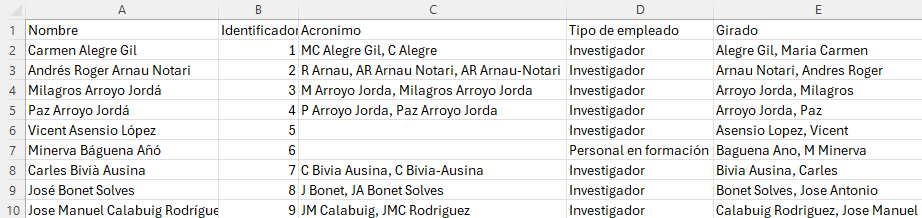
\includegraphics[width=\textwidth]{imgs/Investigadores_internos.png}
\caption{Ejemplo visual de la estructura parcial de \texttt{Investigadores\_internos.csv}.}
\label{fig:ejemplo_investigadores_internos}
\end{figure}

\subsection{Áreas de trabajo}

El fichero \texttt{Areas.csv} recoge el catálogo de áreas de trabajo identificadas a partir de la información pública del IUMPA. Estas áreas se conservaron como información auxiliar asociada a los investigadores y se utilizaron como criterio de filtrado en los grafos de la aplicación.

\begin{table}[H]
\centering
\small
\renewcommand{\arraystretch}{1.25}
\begin{tabularx}{\textwidth}{
>{\raggedright\arraybackslash}p{4cm}
>{\raggedright\arraybackslash}X
}
\toprule
\textbf{Atributo} & \textbf{Descripción} \\
\midrule
\texttt{Area} & Denominación del área de trabajo identificada. \\
\midrule
\texttt{Identificador} & Código interno utilizado para identificar cada área dentro de la base de datos. \\
\bottomrule
\end{tabularx}
\caption{Atributos principales del fichero de áreas de trabajo.}
\label{tab:atributos_areas}
\end{table}

\begin{figure}[H]
\centering
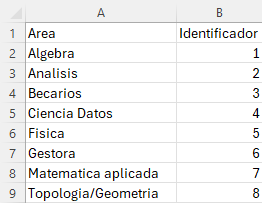
\includegraphics[width=0.3\textwidth]{imgs/Areas.png}
\caption{Ejemplo visual de la estructura del fichero \texttt{Areas.csv}.}
\label{fig:ejemplo_areas}
\end{figure}

\subsection{Revistas}

El fichero \texttt{Revistas.csv} contiene las revistas identificadas a partir de los artículos recopilados. Esta entidad permitió separar la información propia de las revistas de los registros de artículos y reutilizarla tanto en los grafos como en la fase de agrupación semántica.

\begin{table}[H]
\centering
\small
\renewcommand{\arraystretch}{1.25}
\begin{tabularx}{\textwidth}{
>{\raggedright\arraybackslash}p{4cm}
>{\raggedright\arraybackslash}X
}
\toprule
\textbf{Atributo} & \textbf{Descripción} \\
\midrule
\texttt{Revista} & Denominación de la revista o medio de publicación normalizado tras el proceso de depuración. \\
\midrule
\texttt{Identificador} & Código interno utilizado para identificar cada revista dentro de la base de datos. \\
\midrule
\texttt{Editorial} & Editorial asociada a la revista, cuando estaba disponible. \\
\bottomrule
\end{tabularx}
\caption{Atributos principales del fichero de revistas.}
\label{tab:atributos_revistas}
\end{table}

\begin{figure}[H]
\centering
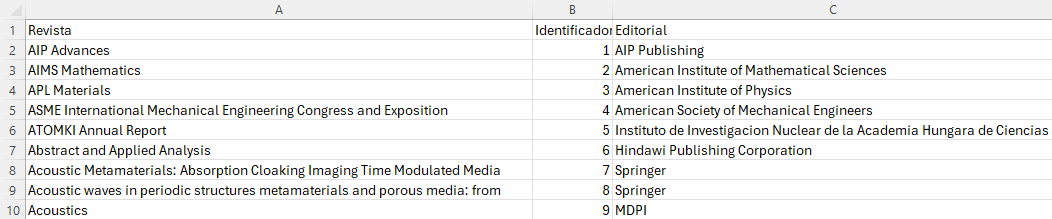
\includegraphics[width=0.85\textwidth]{imgs/Revistas.png}
\caption{Ejemplo visual de la estructura del fichero \texttt{Revistas.csv}.}
\label{fig:ejemplo_revistas}
\end{figure}

\section{Ficheros de relaciones}

Los ficheros de relaciones almacenan los vínculos entre las entidades de la base de datos. Estas estructuras fueron especialmente importantes para la aplicación interactiva, ya que algunas permitieron transformar la información tabular en nodos y enlaces, mientras que otras se utilizaron como información de filtrado.

\subsection{Relación entre investigadores y áreas}

El fichero \texttt{es\_parte\_de\_limpio\_listas.csv} recoge la relación entre investigadores internos y áreas de trabajo. Esta estructura permitió asociar cada investigador con las áreas identificadas en la fuente institucional y utilizar dicha asociación como criterio de filtrado en la aplicación.

\begin{table}[H]
\centering
\small
\renewcommand{\arraystretch}{1.25}
\begin{tabularx}{\textwidth}{
>{\raggedright\arraybackslash}p{4cm}
>{\raggedright\arraybackslash}X
}
\toprule
\textbf{Atributo} & \textbf{Descripción} \\
\midrule
\texttt{Nombre} & Nombre del investigador interno asociado a una o varias áreas de trabajo. \\
\midrule
\texttt{Areas} & Lista de áreas de trabajo vinculadas al investigador. \\
\bottomrule
\end{tabularx}
\caption{Atributos principales de la relación entre investigadores y áreas.}
\label{tab:atributos_es_parte_de}
\end{table}

\begin{figure}[H]
\centering
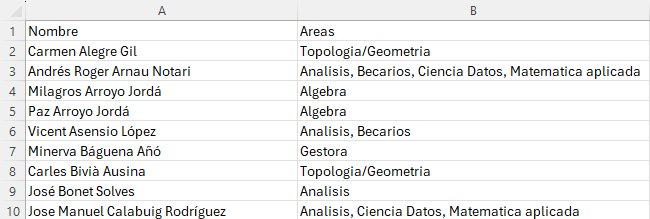
\includegraphics[width=0.85\textwidth]{imgs/es_parte_de.png}
\caption{Ejemplo visual de la estructura del fichero \texttt{es\_parte\_de\_limpio\_listas.csv}.}
\label{fig:ejemplo_es_parte_de}
\end{figure}

\subsection{Relación entre investigadores y revistas}

La relación \textit{ha\_publicado\_en} se almacenó mediante ficheros individuales por investigador. Por ello, el investigador no aparecía como una columna dentro del fichero, sino que quedaba identificado por el propio nombre del archivo. Estos ficheros recogen los artículos asociados a cada persona, la revista en la que fueron publicados y el año correspondiente.

\begin{table}[H]
\centering
\small
\renewcommand{\arraystretch}{1.25}
\begin{tabularx}{\textwidth}{
>{\raggedright\arraybackslash}p{4cm}
>{\raggedright\arraybackslash}X
}
\toprule
\textbf{Atributo} & \textbf{Descripción} \\
\midrule
\texttt{title} & Título del artículo recopilado para el investigador asociado al fichero. \\
\midrule
\texttt{journal} & Revista o medio de publicación asociado al artículo. \\
\midrule
\texttt{year} & Año de publicación del artículo. \\
\bottomrule
\end{tabularx}
\caption{Atributos principales de los ficheros de la relación entre investigadores y revistas.}
\label{tab:atributos_ha_publicado_en}
\end{table}

\begin{figure}[H]
\centering
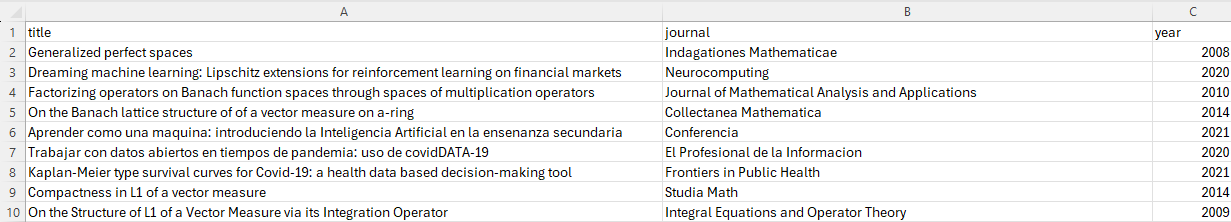
\includegraphics[width=\textwidth]{imgs/ha_publicado_en_JMCR.png}
\caption{Ejemplo visual de un fichero de la relación \textit{ha\_publicado\_en}.}
\label{fig:ejemplo_ha_publicado_en}
\end{figure}

\subsection{Relación de coautoría}

El fichero \texttt{ha\_publicado\_con.csv} recoge los coautores asociados a cada investigador a partir de los artículos recopilados. Esta estructura permitió construir relaciones de colaboración derivadas de artículos compartidos.

\begin{table}[H]
\centering
\small
\renewcommand{\arraystretch}{1.25}
\begin{tabularx}{\textwidth}{
>{\raggedright\arraybackslash}p{4cm}
>{\raggedright\arraybackslash}X
}
\toprule
\textbf{Atributo} & \textbf{Descripción} \\
\midrule
\texttt{nombre} & Nombre del investigador interno para el que se recoge la relación de coautoría. \\
\midrule
\texttt{otros\_inv} & Lista de autores con los que el investigador ha compartido artículos según la información recopilada. \\
\bottomrule
\end{tabularx}
\caption{Atributos principales del fichero de relación de coautoría.}
\label{tab:atributos_ha_publicado_con}
\end{table}

\begin{figure}[H]
\centering
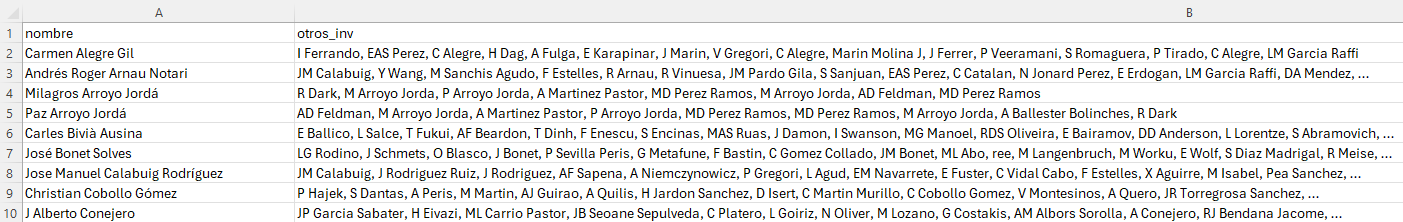
\includegraphics[width=\textwidth]{imgs/ha_publicado_con.png}
\caption{Ejemplo visual abreviado de la estructura de \texttt{ha\_publicado\_con.csv}.}
\label{fig:ejemplo_ha_publicado_con}
\end{figure}

\subsection{Relación entre investigadores y proyectos}

La relación \textit{ha\_participado\_en} se almacenó mediante ficheros individuales por investigador. Por ello, el investigador al que correspondía cada conjunto de proyectos quedaba identificado por el propio nombre del archivo. Estos ficheros recogen los proyectos asociados a cada persona, junto con información sobre sus participantes, fecha, identificador e indicación de investigador principal.

\begin{table}[H]
\centering
\small
\renewcommand{\arraystretch}{1.25}
\begin{tabularx}{\textwidth}{
>{\raggedright\arraybackslash}p{4.2cm}
>{\raggedright\arraybackslash}X
}
\toprule
\textbf{Atributo} & \textbf{Descripción} \\
\midrule
\texttt{TÍTULO} & Título o denominación del proyecto de investigación. \\
\midrule
\texttt{AUTORES} & Lista original de participantes del proyecto, conservando la información de rol cuando aparecía en la fuente. \\
\midrule
\texttt{FECHA} & Fecha asociada al proyecto en la información recopilada. \\
\midrule
\texttt{IDENTIFICADOR} & Código del proyecto dentro de la fuente original. \\
\midrule
\texttt{Es\_IP\_Principal} & Indicador lógico que señala si el investigador asociado al fichero actuaba como investigador principal en el proyecto. \\
\midrule
\texttt{INVESTIGADOR PRINCIPAL} & Nombre del investigador principal del proyecto, cuando estaba disponible. \\
\midrule
\texttt{AUTORES SIMPLIFICADO} & Lista de participantes normalizada, eliminando información sobre el rol para facilitar el tratamiento posterior. \\
\bottomrule
\end{tabularx}
\caption{Atributos principales de los ficheros de la relación entre investigadores y proyectos.}
\label{tab:atributos_ha_participado_en}
\end{table}

\begin{figure}[H]
\centering
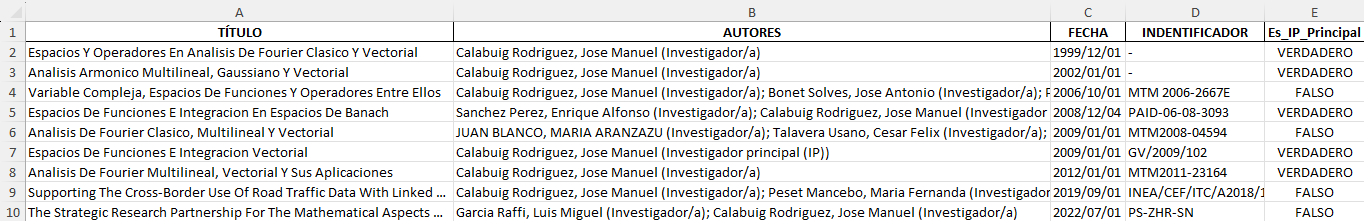
\includegraphics[width=\textwidth]{imgs/ha_participado_en_JMCR.png}
\caption{Ejemplo visual de la estructura parcial de \textit{ha\_participado\_en}.}
\label{fig:ejemplo_ha_participado_en}
\end{figure}

\subsection{Relación de colaboración en proyectos}

El fichero \texttt{ha\_participado\_con.csv} recoge las relaciones entre investigadores derivadas de la participación conjunta en proyectos. Esta estructura permitió representar colaboraciones basadas en proyectos, de forma complementaria a las colaboraciones obtenidas a partir de artículos compartidos.

\begin{table}[H]
\centering
\small
\renewcommand{\arraystretch}{1.25}
\begin{tabularx}{\textwidth}{
>{\raggedright\arraybackslash}p{4cm}
>{\raggedright\arraybackslash}X
}
\toprule
\textbf{Atributo} & \textbf{Descripción} \\
\midrule
\texttt{nombre} & Nombre del investigador interno para el que se recoge la relación de colaboración en proyectos. \\
\midrule
\texttt{otros\_inv} & Lista de participantes con los que el investigador ha coincidido en proyectos según la información recopilada. \\
\bottomrule
\end{tabularx}
\caption{Atributos principales del fichero de colaboración en proyectos.}
\label{tab:atributos_ha_participado_con}
\end{table}

\begin{figure}[H]
\centering
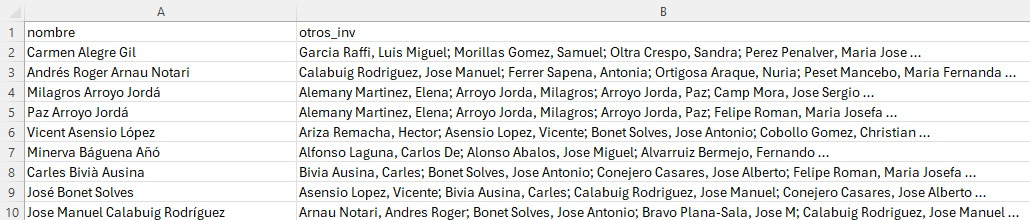
\includegraphics[width=\textwidth]{imgs/ha_participado_con.png}
\caption{Ejemplo visual abreviado de la estructura de \texttt{ha\_participado\_con.csv}.}
\label{fig:ejemplo_ha_participado_con}
\end{figure}

\section{Estructuras auxiliares para el análisis semántico}

Además de los ficheros utilizados para construir los grafos, se generaron estructuras auxiliares destinadas a preparar la fase de agrupación semántica. Estas estructuras permitieron trasladar la información de revistas y palabras clave al nivel de investigador, conservando la trazabilidad del origen de cada término.

\subsection{Matriz de revistas y palabras clave}

El fichero \texttt{One\_Hot\_Palabras\_Revistas\_filtrado.xlsx} representa la asociación entre revistas y palabras clave mediante una matriz de presencia y ausencia. Cada fila correspondía a una revista y las columnas indicaban la presencia de términos temáticos asociados a ella.

\begin{table}[H]
\centering
\small
\renewcommand{\arraystretch}{1.25}
\begin{tabularx}{\textwidth}{
>{\raggedright\arraybackslash}p{4cm}
>{\raggedright\arraybackslash}X
}
\toprule
\textbf{Elemento} & \textbf{Descripción} \\
\midrule
Filas & Cada fila representa una revista incluida en la matriz. \\
\midrule
Columnas & Cada columna, salvo la primera que representa a las revistas, representa una palabra clave temática. \\
\midrule
Valores binarios & Indican la asociación entre revista y palabra clave: 1 representa presencia de la palabra en la revista y 0 representa ausencia. \\
\bottomrule
\end{tabularx}
\caption{Estructura principal de la matriz de revistas y palabras clave.}
\label{tab:atributos_one_hot_revistas}
\end{table}

\begin{figure}[H]
\centering
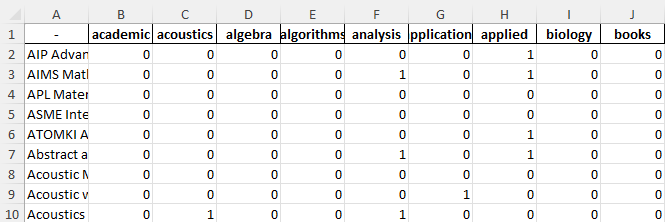
\includegraphics[width=0.75\textwidth]{imgs/one_hot_palabras_revistas_filtrado.png}
\caption{Ejemplo visual parcial de la matriz de revistas y palabras clave.}
\label{fig:ejemplo_one_hot_palabras_revistas}
\end{figure}

\subsection{Matriz de investigadores y palabras clave}

El fichero \texttt{Matriz\_Investigadores\_Keywords.xlsx} traslada la información temática al nivel de investigador. A partir de las revistas en las que había publicado cada persona, se asociaban a cada investigador los términos temáticos correspondientes.

\begin{table}[H]
\centering
\small
\renewcommand{\arraystretch}{1.25}
\begin{tabularx}{\textwidth}{
>{\raggedright\arraybackslash}p{4cm}
>{\raggedright\arraybackslash}X
}
\toprule
\textbf{Elemento} & \textbf{Descripción} \\
\midrule
Filas & Cada fila representa un investigador incluido en la matriz. \\
\midrule
Columnas & Cada columna, salvo la primera que representa al investigador, representa una palabra clave temática. \\
\midrule
Valores binarios & Indican la asociación entre investigador y palabra clave: 1 representa presencia de la palabra y 0 representa ausencia. \\
\bottomrule
\end{tabularx}
\caption{Estructura principal de la matriz de investigadores y palabras clave.}
\label{tab:atributos_matriz_investigadores_keywords}
\end{table}

\begin{figure}[H]
\centering
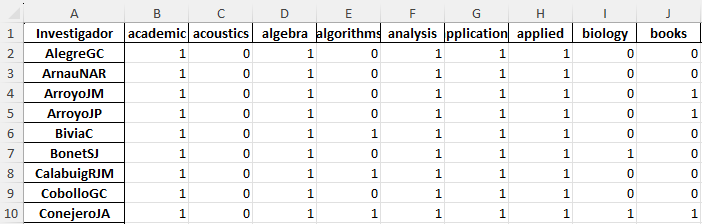
\includegraphics[width=0.8\textwidth]{imgs/matriz_investigadores_keywords.png}
\caption{Ejemplo visual parcial de la matriz de investigadores y palabras clave.}
\label{fig:ejemplo_matriz_investigadores_keywords}
\end{figure}

\subsection{Trazabilidad entre investigadores, revistas y palabras clave}

El fichero \texttt{Trazabilidad\_Keywords\_Revistas.xlsx} conserva la relación entre investigador, revista y palabra clave. Esta estructura permitió interpretar posteriormente el origen de los términos asociados a cada investigador.

\begin{table}[H]
\centering
\small
\renewcommand{\arraystretch}{1.25}
\begin{tabularx}{\textwidth}{
>{\raggedright\arraybackslash}p{4cm}
>{\raggedright\arraybackslash}X
}
\toprule
\textbf{Atributo} & \textbf{Descripción} \\
\midrule
\texttt{Investigador} & Investigador al que se asocia la información temática. \\
\midrule
\texttt{Revista} & Revista de la que proceden las palabras clave asociadas al investigador. \\
\midrule
\texttt{Keyword} & Término temático asociado a la revista y trasladado al perfil del investigador. \\
\bottomrule
\end{tabularx}
\caption{Atributos principales del fichero de trazabilidad temática.}
\label{tab:atributos_trazabilidad_keywords}
\end{table}

\begin{figure}[H]
\centering
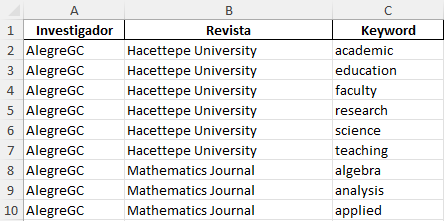
\includegraphics[width=0.5\textwidth]{imgs/trazabilidad_keywords_revistas.png}
\caption{Ejemplo visual parcial de trazabilidad entre investigadores, revistas y palabras clave.}
\label{fig:ejemplo_trazabilidad_keywords}
\end{figure}

\subsection{Listado auxiliar de revistas}

El fichero \texttt{Titulos\_revistas.json} recoge un listado auxiliar de revistas utilizado durante la preparación de la información temática. Este fichero sirvió como apoyo para organizar y consultar los títulos de revistas en la fase previa al análisis semántico.

\begin{table}[H]
\centering
\small
\renewcommand{\arraystretch}{1.25}
\begin{tabularx}{\textwidth}{
>{\raggedright\arraybackslash}p{4cm}
>{\raggedright\arraybackslash}X
}
\toprule
\textbf{Atributo} & \textbf{Descripción} \\
\midrule
Título de revista & Denominación de la revista incluida en el listado auxiliar. \\
\bottomrule
\end{tabularx}
\caption{Atributo principal del listado auxiliar de revistas.}
\label{tab:atributos_titulos_revistas}
\end{table}



%%%%%%%%%%%%%%%%%%%%%%%%%%%%%%%%%%%%%%%%%%%%%%%%%%%%%%%%%%%%%%%%%%%%%%%%%%%%%%%
%
% SI AÑADO MÁS APÉNDICES, MODIFICAR ÚLTIMO PÁRRAFO DE 1.4 Estructura de la memoria
%
%%%%%%%%%%%%%%%%%%%%%%%%%%%%%%%%%%%%%%%%%%%%%%%%%%%%%%%%%%%%%%%%%%%%%%%%%%%%%%%




%%%%%%%%%%%%%%%%%%%%%%%%%%%%%%%%%%%%%%%%%%%%%%%%%%%%%%%%%%%%%%%%%%%%%%%%%%%%%%%
%                              FI DEL DOCUMENT                                %
%%%%%%%%%%%%%%%%%%%%%%%%%%%%%%%%%%%%%%%%%%%%%%%%%%%%%%%%%%%%%%%%%%%%%%%%%%%%%%%


\end{document}